\documentclass[12pt,a4paper,titlepage]{article}
\usepackage[UKenglish]{babel}   % for hyphenation etc.
\usepackage[babel]{microtype}          % for better paragraph look (reduces overfull boxes etc)
  \tolerance=5000             % maybe needed to hinder writing on margin (allows "worse" paragraphs)
\usepackage[utf8]{inputenc}     % so ä,ö, etc. work
\usepackage[T1]{fontenc}        % correct font encoding
\usepackage{DejaVuSerif}        % font (install texlive-fonts-extra) other fonts: cochineal; % also sudo apt install cm-super!
%\usepackage{mathptmx}          % change font: times new roman with math support
%\usepackage{pmboxdraw}          % so boxdrawing chars can be displayed (needed for code inclusion)
%\usepackage{textgreek}          % to have greek letters in text
\usepackage{amsmath}
\usepackage{textcomp}           % for additional signs in T1 fonts
%\usepackage[cal=esstix]{mathalpha}  % for specific calligraphy math font (to better match image from elsewhere). try also esstix, boondoxupr, rsfso
\usepackage{csquotes}           % use so quotes are set in right typeset too
\usepackage[all]{nowidow}        % use package to hinder orphaned sentences at begin/end of page
\usepackage{graphicx}           % to include graphics
\usepackage{float}              % to include float graphics
\usepackage[section]{placeins}  % to contain floats in sections
\usepackage{afterpage}          % to better place figures
\usepackage{subcaption}
\usepackage[table]{xcolor}              % for naming colours (later on), also makes \cellcolor available in table
%tikz picture
\usepackage{tikz}
\usepackage{rotating}
%\usepackage{tikz-uml}
\usetikzlibrary{arrows.meta}
\usetikzlibrary{positioning, fit}
  \usepackage{xspace}              %make space after self defined vars optional (except when , or .)
  \usepackage[hang,flushmargin, bottom]{footmisc}   % no indent in footnotes
  \addtolength{\skip\footins}{-10pt}          % decrease distance to footnotes
\usepackage{perpage}             % to be able to reset footnote numbers per page
\MakePerPage{footnote}       % reset foonote numbers perpage page
\usepackage{titling}            % so \thetitle etc. can be used later
\usepackage[hyphens]{url}       % \usepackage{xurl} for break at any point
\usepackage{hyphenat}           % allow hyphenation at underscores!
  \urlstyle{same}
\usepackage[numbib]{tocbibind}  % to include lists in content
\usepackage{tocloft}            % to make toc and lof/loft pretty
  % add tablename to LoT and adjust indent
  \renewcommand{\cfttabpresnum}{\tablename~}
  \addtolength{\cfttabnumwidth}{50pt}
  % add figurename to LoF and adjust indent
  \renewcommand{\cftfigpresnum}{\figurename~}
  \addtolength{\cftfignumwidth}{50pt}
  \setlength\cftparskip{-2pt}  %smaller skips after sections in toc, adjust listings too
  %no equivalent for listings -> has to be done later with listings package
  %make space between dots smaller
  \renewcommand\cftdotsep{1} % need to adjust listings line too!

\usepackage{setspace}           % for changing line space (e.g. in titlepage)
\usepackage{enumitem}           % reduce spacing in lists (needs to be adjusted according to used spacing)
  \setlist{topsep=-2ex, parsep=0pt}
  % reduce spacing around equations
  \setlength{\abovedisplayskip}{5pt}
  \setlength{\belowdisplayskip}{5pt}
  %re-adjust space after pictures?
  %\setlength{\intextsep}{15pt} % Vertical space above & below [h] floats
  %\setlength{\textfloatsep}{15pt} % Vertical space below (above) [t] ([b]) floats
  \setlength{\textfloatsep}{20pt}  % vertical spacing between figures

\usepackage[font=singlespacing, labelfont={bf,it}, textfont=it]{caption}
% captionskips not working with \restylefloat{figure}, but with \restylefloat*{figure}. However \parskip after in-text float cannot be changed!
% setup bib (use biblatex when using a biblatex-reference file! - biblatex needs biber installed on system
\usepackage[style=alphabetic, url=false, eprint=false, date=year, backend=biber]{biblatex} %other styles: authoryear, ieee, debug(for key printing)
  % make all bibliography acronyms (url, isbn, doi etc, upper case
  % (bibacro is called on all of these, and tries to make it lowercase when possible)
  \renewcommand*{\mkbibacro}[1]{\MakeUppercase{#1}}
  % get rid of pages field (I dont want it in my bibliography)
  \AtEveryBibitem{\clearfield{pages}}
  % fix the breaking space in the \textcite command!
  \renewcommand\namelabeldelim{\addnbspace}
  \setcounter{biburlnumpenalty}{7000} % in bib: allow url breaking after numbers
  %\setcounter{biburllcpenalty}{7000} % in bib: allow url breaking after lower case letter
  %\setcounter{biburlucpenalty}{8000} % in bib: allow url breaking after upper case letter

\usepackage[nomain,acronym,toc,nonumberlist,nogroupskip]{glossaries}    % for list of abbrevations
    \makenoidxglossaries
    % for some reason glossaries does extra spacing after title, remove it.
    %\setglossarypreamble[acronym]{\vspace*{-0.75\baselineskip}}
    \setglossarystyle{long}    % set glossary to table style (or alttree with %\glssetwidest{long-placeholder-word}
    \setlength{\glsdescwidth}{0.8\textwidth}   % make it more narrow, so it matches figures and tables
    \renewcommand*{\glsnamefont}[1]{\bfseries #1} %make names bold 
    \addto{\captionsUKenglish}{     %change title of acronyms
        \renewcommand{\acronymname}{List of Acronyms}
    }



\usepackage{longtable}     % allow tables to span multiple pages with longtable environment
\usepackage{tabularx}      % pretty columns
\usepackage{makecell}      % for specific line breaks in cells
\usepackage{multirow}
  \setcellgapes{5pt}   % set cell gaps in gaped makecell

%setup code snippets
\usepackage{listings}
% since tocloft does not provide options, it has to be crafted manually. Far from ideal, but works at least a bit
\makeatletter
    \renewcommand{\@dotsep}{1}  % change dot distance in listings
    \renewcommand*{\lstlistlistingname}{List of Code}
    \renewcommand*{\lstlistingname}{Code}
    %add name of Codes (and color) before each listing; adjust spacing between number and text to same spacings as Figures and Tables (2.5em)
    \renewcommand{\l@lstlisting}[2]{%
        \@dottedtocline{1}{20pt}{2.5em}{\textcolor{linkcolor}{\lstlistingname\ }#1}{#2}
    }
\makeatother
% needed later to adjust spacing around listings title
\usepackage{titlesec}
    
    \definecolor{codegreen}{rgb}{0,0.6,0}
    \definecolor{codegray}{rgb}{0.5,0.5,0.5}
    \definecolor{codepurple}{rgb}{0.58,0,0.82}
    \definecolor{backcolour}{rgb}{0.95,0.95,0.92}
\lstdefinestyle{mystyle}{
    backgroundcolor=\color{backcolour},
    commentstyle=\color{codegreen},
    keywordstyle=\color{magenta},
    numberstyle=\tiny\color{codegray},
    stringstyle=\color{codepurple},
    basicstyle=\ttfamily\footnotesize,
    breakatwhitespace=false,
    breaklines=true,
    captionpos=t,
    keepspaces=true,
    numbers=left,
    numbersep=5pt,
    showspaces=false,
    showstringspaces=false,
    showtabs=false,
    tabsize=2,
    literate=
        {├}{\textSFviii}{1}%
        {└}{\textSFii}1%
        {│}{\textSFxi}1%
        {─}{\textSFx}1%
        {µ}{\textmu}1%
}
\lstdefinestyle{inlinestyle}{
    backgroundcolor=\color{backcolour},
    commentstyle=\color{codegreen},
    keywordstyle=\color{magenta},
    numberstyle=\tiny\color{codegray},
    stringstyle=\color{codepurple},
    basicstyle=\ttfamily\large,
    breakatwhitespace=true,   %if true, ONLY linebreak at whitespace, so there will be no linebreak at end (and comma in next line)
    breaklines=true,
}
\lstset{style=inlinestyle} %set default, so \lstinline does not need style argument. can be used anywhere in document to change style
%or name an environment, code must be put directly inside
\lstnewenvironment{python}[2]
{\lstset{language=Python,style=mystyle,caption={#1},label={#2}}}
{}

%%%%%%%%%%%%%%%%%%%%%%%%%%%%%%%%%%%%%%%%%%%%%%%%%%%%%%%%%%%%%%%%%%%%%%%%%%%%%%%%%%%%%%%%
%%%%% Document-specific properties (used in pdf, titlepage + references)
\title{Unsupervised Deep Learning for Semantic Segmentation of Scientific 3D~Images}
\author{Jennifer Ahrens}
\addbibresource{./MachineLearning_library.bib}


%% $\lambda_{knn}$ \\%define glossary terms here: % use with \gls{<first arg>}
\newacronym{unisef}{UniSeF}{Universal Segmentation Framework}
\newacronym{ct}{CT}{Computed Tomography}
\newacronym{mct}{~\hspace{-5pt}\textmu{}CT}{Micro-Computed Tomography}
\newacronym{srmct}{SR\textmu{}CT}{Synchrotron Radiation Micro-Computed Tomography}
\newacronym{dsc}{DSC}{Dice Similarity Coefficient}
\newacronym{nsd}{NSD}{Normalised Surface Distance}
\newacronym{mrt}{MRT}{Magnetic Resonance Tomography}
\newacronym{desy}{DESY}{Deutsches Elektronen-Synchrotron}
\newacronym{beegfs}{BeeGFS}{parallel file system optimised for high performance computing}
\newacronym{slurm}{SLURM}{Simple Linux Utility for Resource Management}
\newacronym{stego}{STEGO}{Self-supervised Transformer with Energy-based Graph Optimization}
\newacronym{nnu}{nnU-Net}{no new U-Net}
\newacronym{relu}{ReLu}{Rectified Linear unit}
\newacronym{dino}{DINO}{self-\textbf{di}stillation with \textbf{no} labels}
\newacronym{iou}{IoU}{Intersection over Union}
\newacronym{miou}{mIoU}{mean Intersection over Union}
\newacronym{loo}{LOO}{leave-one-out}
\newacronym{picie}{PiCIE}{\textbf{Pi}xel-level feature \textbf{C}lustering using \textbf{I}nvariance and \textbf{E}quivariance}

%add hypenation for words
\hyphenation{Su-per-vised Learn-ing}
\hyphenation{Semi-Super-vised}
\hyphenation{Con-fi-gu-ra-tion}
\hyphenation{re-so-lu-tion}

%%%%%%%%%%%%%%%%%%%%%%%%%%%%%%%%%%%%%%%%%%%%%%%%%%%%%%%%%%%%%%%%%%%%%%%%%%%%%%%%
% Define commands for recurring things (filenames, variables etc), to be formatted togehter
% misc

% proper Nouns / Names / Brands...
\newcommand{\tensorboard}       {TensorBoard}

% define and format data set names
\newcommand{\formatData}[1]      {\textsf{\large{#1}}\xspace}
\newcommand{\mindataset}       {\formatData{minimal screws dataset}}
\newcommand{\fulldataset}           {\formatData{full screws dataset}}

% define and formatfile and folder names
\newcommand{\formatFile}      [1]{\emph{#1}\xspace}
%my filenames

% define and format variables
\newcommand{\formatCode}      [1]{\texttt{#1}\xspace}
\newcommand{\neginter}           {\formatCode{neg\_inter}}
\newcommand{\posinter}           {\formatCode{pos\_inter}}
\newcommand{\posintra}           {\formatCode{pos\_intra}}

% define and formatting special content
\newcommand{\formatLabel}[1]           {\textit{#1}}


%%%%%%%%%%%%%%%%%%%%%%%%%%%%%%%%%%%%%%%%%%%%%%%%%%%%%%%%%%%%%%%%%%%%%%%%%%%%%%%%%%%%%%%%

%%%% to be removed in end:
\setlength{\marginparwidth}{2cm} % so todos can be displayed in margin
\usepackage[tickmarkheight=0.2cm]{todonotes}
\newcommand{\source}{\todo[color=cyan]{source}}
\usepackage[normalem]{ulem}      % for crossing out text  


%%% FH-Wedel Layout for Bsc-Thesis:
% box around figures and tables (package float)
%\floatstyle{boxed}
%    \restylefloat*{figure}   % change style for float types, arbitrary w/o type
%    \restylefloat*{table}
\onehalfspacing              %set line space (setspace package)
\usepackage[skip=\baselineskip, indent=0pt]{parskip} % space between paragraphs

\renewcommand\footnoterule{\rule{5cm}{0.1pt}} % setup footnote
\setlength{\footnotesep}{1pc}



%%% to be loaded last
\usepackage{hyperref}        % load hyperref last
% TODO change link-color here before printing
\definecolor{linkcolor}{rgb}{0,0,0.5} %{0,0,.5} % darkblue
\hypersetup
{ colorlinks=true
, breaklinks=true
, linkcolor=linkcolor
, menucolor=linkcolor
, urlcolor=linkcolor
, citecolor=linkcolor
, pdftitle={\thetitle -- \theauthor}
, pdfsubject={\thetitle}
, pdfauthor=\theauthor
, bookmarksnumbered=true
, bookmarksopen=true
, bookmarksopenlevel=3
}
\usepackage[a4paper,  % load geometry after hyperref
% FH-Wedel format:
%inner=3.5cm,outer=3.0cm,
%top=3cm,bottom=3cm,
%footskip=1.0cm,
%nicer format:
    inner=3.5cm,outer=3.0cm,
    top=2.5cm,bottom=2.5cm,
    footskip=1.2cm,
    twoside]{geometry}
\usepackage{booktabs}

% after loading hyperref, redefine the displaynames names for autoref of subsetions
\addto\extrasUKenglish{ 	\renewcommand{\sectionautorefname}{Section} 	\let\subsectionautorefname\sectionautorefname 	\let\subsubsectionautorefname\sectionautorefname }


\begin{document}
    %\todo{remove list of todos and todo-package}
%\listoftodos

\begin{titlepage}
    \begin{singlespace}
        \centering
        
\includegraphics[width=.4\textwidth]{pictures/fhw}\\
        \bigskip
        \textsc{\large Department of Computer Science}\\
        \vfill
        \Large Bachelor Thesis\\

        \huge \thetitle \\

        %\Large \\ %for subtitle
        \vfill

        \normalsize
        \begin{tabular}{l l}
            Eingereicht von: & \theauthor                       \\
            
            \\
            Erarbeitet im:   & 7. Semester \bigskip             \\
            Eingereicht am:  & 20.2.2023 \bigskip               \\
            \\
            Referent: & Prof. Dr. Dennis Säring                 \\
            & Fachhochschule Wedel                 \\
            & Feldstraße 143                 \\
            & 22880 Wedel                 \\
            & Phone: (041\,03)~80\,48-41 \\
            & E-mail: dsg@fh-wedel.de \bigskip
            \\
            Betreut von: & Dr. Philipp Heuser                 \\
            & Deutsches Elektronen-Synchrotron                 \\
            & Notkestraße 85                 \\
            & 22601 Hamburg                 \\
            & Phone: (040)~89\,98\,46\,22                 \\
            & E-mail: philipp.heuser@desy.de\\
        \end{tabular}
    \end{singlespace}
\end{titlepage}

\cleardoublepage

\pagenumbering{Roman}
\pagestyle{empty}
\section*{Abstract}
\addcontentsline{toc}{section}{Abstract}
%setting and problem
Scientific imaging plays a major role in many clinical applications and biomedical studies. 
These scientific images must be analysed and often structures of interest need to be localised and labelled, a process called segmentation.
%Image segmentation is not trivial.
Usually, domain experts are needed to manually annotate data sets in a time-consuming process.
Fortunately, currently more and more unsupervised algorithms become available, which can be trained on data for which no ground truth is available.
However, most of the available unsupervised algorithms are optimised for photographs and applicability to high-resolution scientific images has not been shown.
The aim of this study thus was to investigate the applicability of the unsupervised algorithm ``\gls{stego}'' to high-resolution scientific imaging data, and to understand how to select and prepare scientific imaging data to be used successfully (if possible) with this algorithm.

% experiments
For this the direct transferability of pretrained models was investigated, as well as the performance of models re-trained on a scientific data set, and the effect of different cropping schemes.
%results & discussion
%exp 1
Predicting a scientific data set with models trained on photographs did not yield satisfactory results.
Even though the \gls{miou} values were in the same range as the \gls{miou} of the validation set of the models (around 0.21-0.24), examining the raw predictions showed that labels were not retained sufficiently.
%The similar \gls{miou} rather highlights the deficiency of the metric, then indicate a comparable good result.
% exp 2
When predictions were done on models trained with the same data set, \gls{miou} improved significantly to about~0.5.
Albeit some areas of the images could be segmented well, the obtained segmentations are not yet usable for quantitative scientific analysis.
No definitive proposition regarding cropping regime could be made.

% conclusion
Given that \gls{stego} is an unsupervised algorithm, results are impressive.
Further experiments, in particular a retraining of the backbone with a huge scientific data set, may even yield results fit for scientific analysis.
Overall, unsupervised segmentation is a rapidly advancing field with promising results, even though this recent algorithm is not yet in a state suitable for scientific use-cases.
% Keeping in mind that this study was only a very rough try, it can be expected that better results are possible in the future.



\cleardoublepage

\pagestyle{plain}
\tableofcontents
\newpage %TODO manual adjustment, check
\listoffigures
\newpage %TODO manual adjustment, check
\listoftables
%\addcontentsline{toc}{section}{\lstlistlistingname}
%change spacing around title for list of code
%\titlespacing*{\section} {0pt}{2.5ex}{4.5ex}
%\lstlistoflistings      %list of code-snippets
%\titlespacing*{\section} {0pt}{3.5ex plus 1ex minus .2ex}{2.3ex plus .2ex} % reset to default
\printnoidxglossaries   % must be used with noidx, else nothing is displayed

% because my glossary style is a table, counter needs to be resetted
\setcounter{table}{0}
\newpage
\pagestyle{plain}
\pagenumbering{arabic}
\clearpage
\section{Introduction}\label{sec:introduction}
%importance of medical imaging
%In medicine visualising what is hidden is crucial.
Scientific imaging plays a major role in many clinical applications and biomedical studies~\autocite{Ganguly2010}.
The benefits are obvious: today, generating three-dimensional high resolution images of the inside of an object is fast, non-invasive, and relatively simple, as explained later.
Thus, nearly everything can be imaged using \gls{ct} or \gls{mrt}.
Imaging is extensively used in medical disciplines such as oncology, neuroscience, cardiology, and many more, to localise tumours, thrombosis or haemorrhage, visualise whole brain areas, or even identify specific cell types in different tissues~\autocite{Ganguly2010}.
But it is also used in biomedical and material science, where often techniques are utilised that go beyond off-the-shelf medical instruments like \glsfirst{srmct}, which is done extensively at \gls{desy}. %\footnote{At \gls{desy} the Petra III beam lines are operated by HEREON, for example to develop implants that can be absorbed by the body over time~\autocite{Baltruschat2021}}

%problem of medical imaging
While taking these images can (often) be considered a well-defined routine task, processing them however has proved to be a major challenge.
The images must be analysed and structures of interest need to be localised and labelled, a process called segmentation.
Usually, this is done manually, which takes a lot of time, and often domain experts like medical personnel or physicians are needed to identify specific structures~\autocite{Litjens2017}.
Fortunately, in the last years more and more deep learning techniques became available for medical image segmentation, reducing the time and human effort needed to achieve good segmentation results~\autocite{Antonelli2022}.
However, most algorithms are supervised and still rely on at least some segmented input data~\autocite[e.g.][]{Antonelli2022}, which means that still a lot of manual labor must be invested.
Especially for scientific research, this is a major problem since samples wildly differ between experiments, and models can not be reused.
For example at the microtomography beamline at \gls{desy}, scanned samples range from biological specimen like prehistoric amber or bone implants, to material samples, like surfaces of solar panels.
Currently, segmentations take days, even though algorithms are used to do it automatically, as these still require manually labelled training data.

%Aim of study
Only recently an unsupervised algorithm has become available, which does not rely on already labelled data: \glsfirst{stego}~\autocite{Hamilton2022}.
Using an unsupervised algorithm would save days during the evaluation of experiments at \gls{desy}.
Given the promising results of \gls{stego} for standard data sets, the aim of this bachelor thesis thus is to investigate \gls{stego}s applicability and transferability to high-resolution scientific data.
Since the algorithm was developed to segment two-dimensional photographs, some adaptions need to be made, in order to use it with high-resolution, three-dimensional scientific imaging data.
The main delivery of this study thus will be the adapted \gls{stego} as well as insights about using scientific data sets for training, and how to select hyper- and model-parameters for using \gls{stego} with these kinds of imaging data.

%structure of this paper:
The paper is structured as follows:
To understand how deep learning helps in image segmentation, first the scope and issues of image segmentation will be defined, followed by a broad introduction to deep learning and neural networks.
The main focus will be on transformers, algorithms that use an attention mechanism to derive semantic from an input.
Especially \gls{stego}~\autocite{Hamilton2022} will be explained, a transformer-based algorithm successfully used to segment 2D photographs unsupervised.
In the next section the adaption of \gls{stego} to 3D high-resolution scientific imaging data is documented, and experiments to evaluate it in the scientific imaging context are introduced.
%The experiments are designed to determine the influence of the training data, especially concerning data set diversity.
%Additionally, it will be investigated if overclustering helps to resolve difficult labels.
%Qualitative assessment will be done by comparing predictions to the ground truth.
Results will be presented and discussed, and, finally, the potential of \gls{stego} for unsupervised segmentation of scientific imaging data will be assessed.

\section{Image Segmentation}\label{sec:segmentation}
%\url{https://en.wikipedia.org/wiki/Image_segmentation#Trainable_segmentation}

%Segmentation is one of the most often automated medical imaging task~\autocite{MaierHein2018}.
In 2018, 70~\% of all biomedical image processing algorithms tried to solve the problem of image segmentation~\autocite{MaierHein2018}.
Segmentation is the process of partitioning images into multiple semantic sets of pixels (segments), for example to exactly locate objects within the image~\autocite{Szeliski2021}.
In the biomedical context, this could be outlining tumour boundaries, differentiating organs, vessels, and bones, locating metastases, or simply validating the position of implants.

\begin{figure}[!htb]
    \centering
    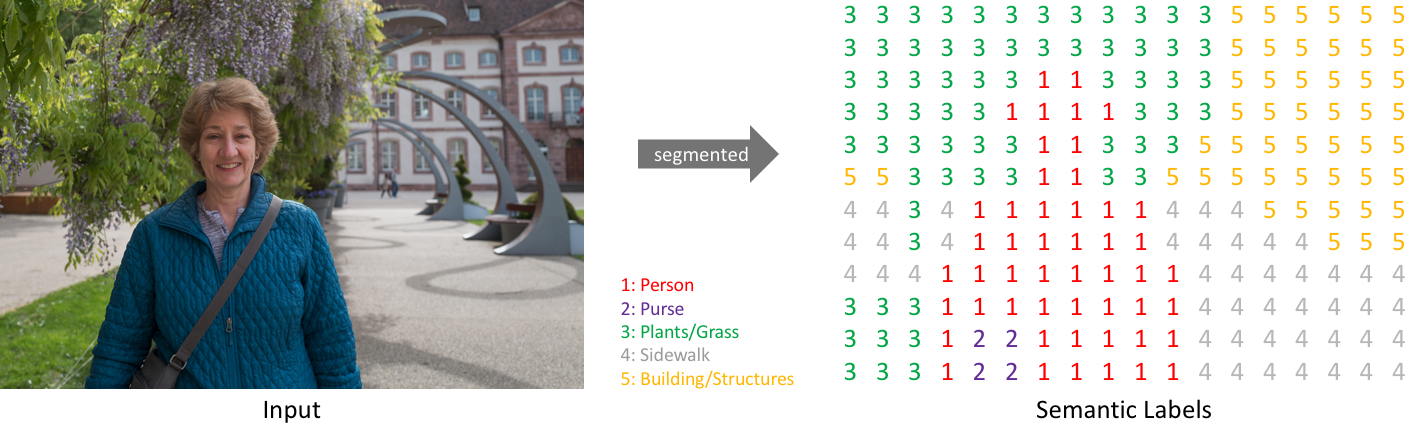
\includegraphics[width=\textwidth]{pictures/semantic-labels}\\
    \caption[Segmentation Map: Image and Labels]{Visualisation of an image and its segmentation map, containing the class labels of the pixels. For simplicity, a lower resolution segmentation map is shown. In reality, the resolutions match each other. Figure from~\autocite{Jordan2018}.}
    \label{fig:semantic-segmentation}
\end{figure}

%Definition
Segmentation is done by assigning a class label (usually an integer) to each pixel of an image.
These labels can be collected in a segmentation map of the same size as the image, as seen in \autoref{fig:semantic-segmentation}.
%classes of segmentation
Generally, segmentation is differentiated into semantic and instance segmentation.
In semantic segmentation, the same class is assigned to each object of the same type.
So, objects of the same class have the same label.
Instance segmentation differentiates between objects of the same class.~\autocite{Szeliski2021}

%used data and accompanying problems
Especially in scientific image processing, segmentation is a major challenge, since often diminutive structures are of interest and image quality is limited and highly variable, as imaging needs to be non-destructive and is often done in-vivo.


\subsection{Imaging Methods} \label{subsec:3d-imaging-data}
Today, two modalities are mainly used to generate 3D images of scientific samples without destroying them in the process: \glsfirst{ct} and \glsfirst{mrt}~\autocite{Ganguly2010}.
\gls{ct} utilises X-rays to generate an image of a sample, while \gls{mrt} is based on magnetic resonance of atoms in the body~\autocite{Pandit2014,Bercovich2018}.
Generally speaking, \gls{mrt} is better at differentiating soft tissues, while \gls{ct} is better suited to resolve bone structures, since it relies on X-rays, which are density dependent~\autocite{Bercovich2018}.
Additionally, \glspl{ct} can accomplish higher resolutions, especially when using specialised methods like \glsfirst{mct} or \glsfirst{srmct}~\autocite{Pandit2014}.

\subsubsection{Computed Tomography}\label{subsubsec:computed-tomography}
In a \gls{ct}, samples are rotated through the beam (or, in the case of patients, the beam is rotated around the sample) and the 2D intensity pattern of the emerging beam is recorded, indicating the distribution of materials in the sample~\autocite{Bercovich2018}.
Millions of 2D pictures are taken from various positions and angles and are then used to reconstruct a 3D image of the sample by means of reconstruction algorithms (see~\autoref{subsec:data-pre-processing}).
During reconstruction, noise and artifacts from scanning can often be partially removed, but the remainders impede data quality and thus segmentation results~\autocite{Vidal2005}.

%SRµCT
Four main properties have been found to significantly enhance data quality in \glspl{ct}: parallel geometry, monochromaticity, high beam intensity and the propagation phase approach~\autocite{Tafforeau2006}.
All of these properties can be utilised in \glsfirst{srmct}.
The parallel geometry of a synchrotron, where all beams travel parallel instead of conical (as in a traditional \gls{ct}), leads to a much more exact reconstruction.
In addition, the high-energy beams derived from an electron synchrotron make it possible to filter the beam to use monochromatic X-rays, which prevent artifacts from beam hardening (brightening of sample borders and linking of dense structures)\footnote{Beam hardening occurs, because low-energy beams are absorbed more than high-energy beams (thus creating a ‘harder’ beam), generating artifacts, which need to be managed on a case-by-case basis after reconstruction.}.
The high beam intensity found in \gls{srmct} also leads to shorter exposure times (fractions of a second per slice) and thus shorter measuring times with very good resolutions.~\autocite{Tafforeau2006}

In summary, the advantage of \gls{srmct} in comparison to \gls{ct} is the beam intensity: in the former, it is high enough to use monochromatic X-rays, which are able to resolve even finer structures.
And so \gls{srmct} has become one of the most valuable tools in scientific studies.
However, two of the major problems of \gls{srmct} are availability and cost. 
There are only a few synchrotrons globally that reach sufficient beam intensity and so beamline-time is not easy to get.\footnote{Due to a collaboration with Hereon, who operates the Petra III beam lines at \gls{desy}, availability of \gls{srmct} data is not a problem in this study.}

\subsubsection{Magnetic Resonance Tomography}\label{subsubsec:magnetic-resonance-tomography}
\gls{mrt} is not based on passive absorption spectra, but on emissions from protons within the sample.
First, a fixed magnetic field is produced around the sample.
Then, radio frequency pulses are used to excite protons within the sample.
Once the protons relax back to a resting state, they emit a signal that is captured to create an image.~\autocite{Bercovich2018}

\gls{mrt} is superior to CT in soft tissue contrast and is used in nearly all medical domains, as it is often faster and does not use ionising radiation which is harmful in high doses.
Thus, it has become the main tool in oncology and examinations of the heart and brain.~\autocite{Bercovich2018}

\subsection{Data Pre-Processing}\label{subsec:data-pre-processing}
%data preparation
Before images can be used for segmentation, they have to be reconstructed from the 2D absorption spectra (in case of \gls{ct}) or emitted signal maps (in case of \gls{mrt}).
This is done by using specialised software, which also removes artifacts from scanning.
Additionally, images are re-sampled to achieve an even voxel\footnote{A voxel is a three-dimensional pixel.} spacing on all three axis, and normalised to reduce noise and get comparable data sets, not biased by their absolute voxel values~\autocite{Rorden2012}.
In the case of \gls{mrt}-data, normalisation is done on a per-image basis as voxel values are relative.
For \gls{ct}-data, normalisation may be done globally over all data sets, since voxel values are quantitative and reflect physical properties of the data set~\autocite{Isensee2019}.


\subsection{Segmentation Techniques} \label{subsec:problems-in-segmentation}
Traditionally, image segmentation was done with feature-based methods, which rely on properties like pixel value, or gradients (e.g.~watershed method, graph cut techniques or region growing), which need to be defined and selected arbitrarily by a human~\autocite{Kar2021}.
Due to the nature of medical images, they often suffer from low contrast, high spatial variability and scanning artifacts.
Thus, these traditional algorithms are often inaccurate, time-consuming and a lot of manual corrections needs to be done.

In recent years however, deep learning techniques were successfully used to automatically segment images, often even outperforming manual segmentation done by human experts in accuracy and in speed~\autocite{Antonelli2022}.
Deep learning techniques have the ability to improve the accuracy of the model automatically through experience~\autocite{Mitchell1997}, without being explicitly programmed to do so, thus they have the potential to be faster while requiring less human intervention.

For image processing, and even live video segmentation one of the most promising unsupervised deep learning algorithms of the last years is \gls{stego}, a transformer-based architecture, which was found to perform better than the current state-of-the art for unsupervised segmentation~\autocite{Hamilton2022}.
In this study, \gls{stego} will be adapted to be used with high-resolution scientific imaging data.

\section{Deep Learning for Image Segmentation} \label{sec:deep-learning-and-neural-networks}
In the following section, a short introduction to deep learning and especially neural networks and (vision) transformers will be given in order to understand how \gls{stego} can be adapted for scientific data.
In deep learning, multilayer neural networks (or deep neural networks) are used to solve a wide variety of tasks, ranging from classification and clustering to discovering relationships between features of examples (i.e.\ regression), or dimensionality reduction~\autocite{Sarker2021}.
Since image segmentation is just a multilevel pixel classification, it can be easily cast into a deep learning problem, and some algorithms were even found to exceed human performance in quality and time~\autocite{Alzubaidi2021}.

\subsection{Algorithm Categories}
Traditionally, algorithms are classified into three categories:
supervised algorithms, trained on data where ground truth is available, unsupervised algorithms, where ground truth is not available, and reinforcement learning, which is tailored to solve problems where the decision-making process is sequential.
In the last years, also semi-super\-vised algorithms were differentiated, which combine supervised and unsupervised learning, which try to get the best of both worlds.
They are used on data where ground truth is available only on some samples.~\autocite{Burkov2019}

Image segmentation can be done with all three of them, but to date the best results are reached with supervised algorithms like convolutional neural networks or U-Nets~\autocite[e.g.][]{Isensee2019}.
%, though Unsupervised and Semi-supervised Learning are also found increasingly successful~\autocite[e.g.]{VanGansbeke2021}.\footnote{Reinforcement Learning on the other hand, is better tailored to solve problems where the decision-making process is sequential (for example when playing video games or in navigation).} %Reinforcement can be used for segmentation, but that is not classical application https://arxiv.org/abs/2002.06583
%disadvantages of Supervised algorithms and transition
However, these supervised networks do come with a major disadvantage: their need for labelled data.
As it is in the nature of labels to be assigned manually (and for scientific images often even by domain experts which are rare), data preparation takes a lot of time, which is usually not feasible.

%unsupervised learning
This is why today, there are increasing efforts to leverage unsupervised learning techniques, which find an arbitrary structure within the input without getting feedback from ground truth labels~\autocite{Burkov2019}.
Only recently, unsupervised Deep Learning algorithms for image segmentation were presented for 2D pictures, either based on a convolutional neural network~\autocite{VanGansbeke2021} or a vision transformer~\autocite{Caron2021}.
But to date, no unsupervised algorithm is available for scientific imaging data.


\subsection{Deep Neural Networks}
All deep learning algorithms rely on multilayer neural networks.
Originally, artificial neural networks were based on the idea to model biological neurons and especially the connection of neurons (since the connections carry the real information), to enable computers to learn in the same way humans do~\autocite{Ertel2017}.
Today, they are used for a wide variety of tasks, ranging from classification, and clustering, over regression, to dimensionality reduction~\autocite{Sarker2021}.

% how multilayer networks work (roughly)
Multilayer networks are created by using the output of a set of neurons (the layer) as input for the next layer of neurons~\autocite[Chapter~4.2]{Skansi2018}.
Usually, there are no interlayer connections and all neurons of the previous layer are connected to all neurons of the next layer, but this may change with the network architecture~\autocite[Chapter~1.2.2]{Aggarwal2018}.
Each neuron is appointed a set of weights which is multiplied with the input(s) to calculate the output of that neuron~\autocite[Chapter~4.2]{Skansi2018}.
This is done throughout all layers (forward pass).
On the backward pass, the learning is done by purposefully adjusting the weights, so the output of the network will be closer to the desired output~\autocite{Ruder2017}.
In supervised networks, this is done by comparing the output with the label of the training example by means of a loss function~\autocite{Aggarwal2018, Ruder2017}.
In unsupervised networks, the loss function utilises other indicators, as explained exemplarily in~\autoref{sec:stego} for a transformer.
For more details on neural networks, backpropagation and loss functions, see~\autocite[e.g.][]{Pouliakis2016, Sharma2020, Ruder2017}.


\subsection{Model Performance Assessment} \label{subsec:model-performance-assessment}
Once training of a network is finished, and all weights are optimised, the network represents a model, which can be used to predict results for unknown input.
To assess model performance, predictions on a data set not part of the training set are compared to their ground truth~\autocite{Aggarwal2018}.

For classification tasks, the most frequently used assessment metrics rely on the confusion matrix~\autocite{Reinke2022}.
This matrix has two axis, comprising the predicted and actual labels (ground truth), as seen in \autoref{tab:confusion-matrix}.
In a binary classification task, four cardinalities are defined, but it can be easily extended for multilevel classifications by adding a row and column for each label~\autocite{Reinke2022}.
Cardinalities are:
\begin{itemize}
    \item true positives (TP): examples that are correctly predicted to belong to a specific label
    \item false positives (FP): examples that are incorrectly predicted to belong to a specific label
    \item true negatives (TN): examples that are correctly predicted as not belonging to a specific label
    \item false negatives (FN): examples that are incorrectly predicted to not belong to a specific label
\end{itemize}
\vspace{12pt}

\begin{table}[!htb]
    \centering
    \caption[Confusion Matrix for Binary Classification]{Confusion matrix for a binary classification task with the labels \emph{yes} and \emph{no}. It characterises the capabilities of a model by comparing the numbers of actual and predicted examples for each label. The sum within a row gives the number of actual examples with that label, the sum of a column the number of actually predicted examples of that label. The four cardinalities of the table (true positive, false positive, true negative, false negative) are used to calculate metrics that indicate the model performance.}
    \label{tab:confusion-matrix}
    \makegapedcells
    \begin{tabular}{cc|c|c}
        \multicolumn{2}{c|}{}  &   \multicolumn{2}{c}{\textbf{Predicted}}  \\
        &             &      yes       &      no         \\
        \cline{1-4}
        \multirow{2}{*}{\rotatebox[origin=c]{90}{\textbf{Actual}}}
        & yes         & \makecell{true positive \\ (TP)}  &  \makecell{false negative \\ (FN)} \\
        \cline{2-4}
        & no          &  \makecell{false positive \\ (FP)} &  \makecell{true negative \\ (TN)}   \\

    \end{tabular}
\end{table}

%semantic image segmentation assessment score:
The values of the confusion matrix can be used to calculate different metrics, for example the accuracy, but also the \gls{dsc} and the \gls{iou}, which are two of the most commonly used metrics in computer vision and medical image segmentation tasks~\autocite{Reinke2022}.

% Accuracy
In image segmentation, the accuracy represents the proportion of correctly identified pixels.
It is calculated as follows:
\begin{equation}
    Accuracy = \frac{TP + TN}{TP + TN + FP + FN}
    \label{eq:accuracy}
\end{equation}
%DSC
The \gls{dsc} (or F1-score) indicates the overall overlap between the predicted and the actual labels of all pixels (or voxels) as value from 0 (no overlap) to 1 (full overlap)~\autocite{Reinke2022}.
For a single label it is defined as:
\begin{equation}
    DSC = \frac{2TP}{2TP + FP + FN}
    \label{eq:dsc}
\end{equation}
%IoU
The \gls{iou} (or Jaquard-index) is defined as the ratio of area of overlap and area of union, hence the name~\autocite{Reinke2022}:
\begin{equation}
    IoU = \frac{TP}{TP + FP + FN} \text{ or } IoU_{A,B} = \frac{|A \cap B|}{|A \cup B|}
    \label{eq:IoU}
\end{equation}
\gls{iou} and \gls{dsc} are related, as the \gls{dsc} of two sets $A$ and $B$ can also be expressed via the \gls{iou} of these sets~\autocite{Reinke2022}:
\begin{equation}
    DSC_{A,B} = \frac{2IoU_{A,B}}{1 + IoU_{A,B}}
    \label{eq:dsc-IoU}
\end{equation}
When evaluating these metrics, it has to be taken into account, however, that it is just an average and it may be especially misleading when small areas are compared, where a difference of one pixel has a high impact~\autocite{Reinke2022}.
Moreover, it has to be kept in mind that even domain experts often disagree on the exact boundaries of objects in an image~\autocite{Webb2021}.
So when evaluating a model, it is imperative to not rely solely on the metrics, but also have a look on the predictions made.
% limitations of metrics
%When selecting a metric to evaluate a model, the different advantages and limitations must be considered with respect to the task at hand, as explained by~\autocite{Reinke2022}.

% cross validation
Other ways to improve model performance are resampling methods.
In the most basic set-up, available data will be split into train and test set.
The model will be trained on the training set and validation metrics will be calculated on the test set to estimate the model performance (the model's generalisation capacities).
This leaves out a considerable amount of data from the training, and might bias the resulting model.
To mitigate this, often resampling methods are used, where multiple models are trained on different train test splits.
The analysis of these models estimates the performance of the final model (trained on the full data set).
Usually, in machine learning, the so-called k-fold cross validation is done, where the data is split into $k$ sets (or folds) and every fold is used as validation set exactly once.
In practice, $k$ is often set to 5 or 10, depending on the amount of data available.~\autocite[Chapter 5]{James2013}

A special case of cross-validation is leave-one-out cross-validation, where the data set is split into $n$ folds ($n$ indicating the number of samples in the data set).
So, $n$ models are trained, and during each training exactly one sample is used as validation set~\autocite[Chapter 5]{James2013}.
Especially with smaller data sets, a leave-one-out tactic is often recommended, since the algorithm is trained on a more representative training set, thus reducing the bias of the model~\autocite[Chapter 5]{James2013}. %https://codesachin.wordpress.com/2015/08/30/cross-validation-and-the-bias-variance-tradeoff-for-dummies/
However, using only one sample as validation set might lead to a higher variance during evaluations, since inhomogeneities and outliers in the data will have more influence when used alone for validation~\autocite[Chapter 5]{James2013}.
On the other hand, \citeauthor{Bengio2004} found that high correlation of training sets may also lead to a higher variance in leave-one-out cross-validation~\autocite{Bengio2004}. %https://stats.stackexchange.com/questions/61783/bias-and-variance-in-leave-one-out-vs-k-fold-cross-validation
So performance on leave-one-out cross-validation might vary highly between data sets.

\subsection{Transformers}
\label{subsec:transformer}
% http://nlp.seas.harvard.edu/2018/04/01/attention.html#position-wise-feed-forward-networks
% Transformer - Overview
Originally, transformers were developed for (supervised) language processing tasks.
They generally accept sequential input data (e.g.~words in a sentence), while allowing parallel processing.
This sets them apart from the former state-of-the-art in natural language processing (e.g.~recurrent or convolutional neural networks).
In contrast to most other networks, transformers are solely based on an attention mechanism, which can easily be parallelised, and require less computational power, which means they often reach better results with less resources.
Like all encoder-decoders, transformers map an input token\footnote{In this context, a token usually is a word.} to an output token via an intermediate representation of inputs, which should encode all relevant features.~\autocite{Vaswani2017}

% Transformers for images
Due to their good performance, transformers were soon adapted to be applied to image classification, and are today also successfully used as vision transformers for image segmentation tasks~\autocite{Han2023}.
In contrast to most state-of-the-art image segmentation methods, vision transformers have the potential to be trained fully unsupervised~\autocite{Hamilton2022}, making them highly relevant for scientific application, where often no labeled data is available.
However, vision transformers were found to require more data in comparison, as discussed in~\autocite{Coccomini2021}.

\subsubsection{Model Structure}
% Transformer - Model Structure
% https://www.wikiwand.com/en/Transformer_(machine_learning_model)#Architecture
As seen in \autoref{fig:transformer}, transformers implement an encoder-decoder model structure without using convolutions or recurrence, which is instead replaced with multi-head attention and point-wise feedforward networks~\autocite{Vaswani2017}.
\begin{figure}[p]
    \centering
    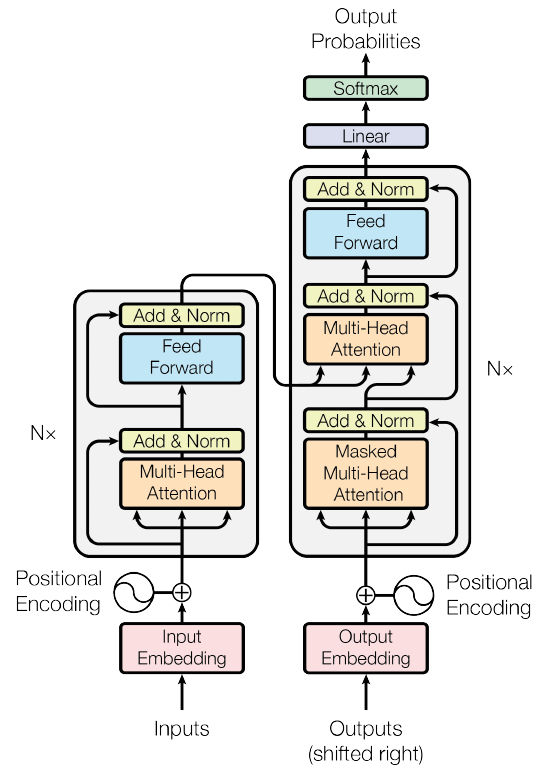
\includegraphics[width=0.75\textwidth]{pictures/transformer}\\
    \caption[Transformer Model Structure]{Transformer model structure. The transformer consists of an encoder (left side) and a decoder (right side). The encoder comprises a multi-head self-attention sublayer and a fully connected feedforward sublayer. Each sublayer has residual connections to the respective input, which is added to the output. The sum is then normalised and passed on to the next sublayer.\\The decoder is structured similarly, but has an additional intermediate layer, where cross-attention with the encoder output is calculated. Also the self-attention sublayer in the decoder is masked, to prevent positions from attending to subsequent positions. The last step in the decoder is a linearisation and softmax application, so the output will be probabilities per token.\\ Inputs and outputs are embedded via a learned function (with shared weights) and get a positional encoding (based on sine and cosine functions). In the decoder, the output embedding is shifted right, again to ensure that predictions only depend on former positions. Figure from~\autocite{Vaswani2017}.}
    \label{fig:transformer}
\end{figure}

% Encoder
The encoder consists of a stack of six layers, each of which contains a multi-head self-attention mechanism and a simple positional-wise fully connected feedforward network~\autocite{Vaswani2017}.
The attentions are passed to this network to transform them to a rich representation~\autocite{Vaswani2017}.
This will adjust for bad initialisation parameters and also hinder rank collapse. %https://theaisummer.com/transformer/
\citeauthor{Geva2021} even found that the feedforward layer actually acts as key-value store~\autocite{Geva2021} (for an explanation of keys and values see~\autoref{subsubsec:attention-mechanism}).
A residual connection of the previous sublayer is added to the result of each sublayer before normalisation is applied~\autocite{Vaswani2017}.
These residual connections and normalisation help to mitigate the vanishing gradient problem~\autocite{Wang2019}. %, and also ensure that the contextual representations of the (original)input tokens actually represent the tokens https://stats.stackexchange.com/questions/565196/why-are-residual-connections-needed-in-transformer-architectures

% Decoder
Like the encoder, the decoder also consists of a stack of six layers, but additionally has a middle sublayer, where multi-head attention over the output of the encoder stack is done.
Additionally, the multi-head attention sublayer is modified to prevent positions from attending to subsequent positions by masking the corresponding inputs.
This, and shifting the output embedding by one position, ensures that predictions for a token can only depend on the positions before that token.
The decoder output is converted to predictions (the probability of the next token) by applying a learned linear transformation with a softmax function.~\autocite{Vaswani2017}

% Token embedding
The input and output tokens are embedded\footnote{Embedding: "translating" higher dimensional tokens to lower dimensional spaces. E.g. converting a token (a word) to a vector.} using a learned function~\autocite{Vaswani2017}.
The embedding layers share their weights with the linear pre-softmax layer of the output, since it was found that this enhances embedding quality~\autocite{Press2017}.
%positional encoding (this was formerly done with convolution / revurrence)
Additionally, the resulting vectors are encoded positionally.
Since skipping convolution and recurrence completely, the position of tokens needs to be coded explicitly, so the order of the sequence can be used by the algorithm.
This is done by mapping the positions to a sinusoid function and adding them to the embedded token, as it is theorised, that this will help the model learn relative positions~\autocite{Vaswani2017}.

%? training and loss function
Training is done via backpropagation~\autocite[e.g.][Chapter~3]{Aggarwal2018}.
During training the weights for the embedding layers, the feedforward layer weights and the weight matrices to calculate Q, K, V (as explained in~\autoref{subsubsec:attention-mechanism}) in encoder and decoder, and the weights to the final linear layer are adjusted~\autocite{Vaswani2017}.
The loss function to be optimised is the cross-entropy loss, which is often used for probability distributions in supervised learning~\autocite[Chapter~1.2.2]{Aggarwal2018}.
%Loss-function of transformer is cross-entropy loss: https://jalammar.github.io/illustrated-transformer/

\subsubsection{Attention Mechanism}\label{subsubsec:attention-mechanism}
%Attention-mechanism: Scaled-Dot-Product 
% https://data-science-blog.com/blog/2021/04/07/multi-head-attention-mechanism/
Attention draws global dependencies between input and output tokens, and re-weights the input tokens, to predict the most probable next token. %, thus enabling the Transformer to predict the most probable output for a token (e.g.~a word), based on the previous inputs.
This is done by mapping a query and a set of key-value pairs to an output.
Queries, keys and values are vectors, that are enclosed using the embedding layer.
In this context, a query represents an input token, keys represent output tokens, and values the respective output tokens belonging to the keys (for example in translations, the keys and values are words of different languages\footnote{In the self-attention layer, key and values are words from the same language for translation tasks.}). %propotional retrival of values, according to their associated keys
Keys and values can stem from the same (self-attention) or former layers (middle sublayer of the decoder).
% selfattention: q, k, v from self; else: q from target, k and v from source!
The attention (for all values for a query-token) is computed as weighted sum of the values of all keys, with the weights calculated from the compatibility of query and keys via the dot product.
%The result is a rewieghted token.
The result is a vector denoting the attention for the given query for each of the tested keys, indicating how probable query and key belong together in the current context. % words (queries) that are often found in vairieng context (with multiple different values following them) should not have high attention scores related to these varieng words)
This calculation is repeated for all queries and the results are stacked to an attention matrix.~\autocite{Vaswani2017}

This attention function can be computed efficiently in parallel for multiple queries by combining queries, keys, and values into matrices $Q, K$ and $V$, and applying scaling and a softmax function for normalisation~\autocite{Vaswani2017}:
\begin{equation}
    Attention(Q,K,V)=\underbrace{softmax\left(\frac{Q K^T}{\sqrt{d_k}}\right)}_{attention~map} V
    \label{eq:KQV}
\end{equation}
% attention map = where to look, V = what you get, when you look there

For multi-head attention, this function is executed multiple times in parallel, each with a slightly different projection of the query, keys, and values.\footnote{The weights to get these projections are also trained in the backwards phase.}
The final result is combined from these projections.
This allows the model to utilise information from multiple representation subspaces and positions.~\autocite{Vaswani2017}
% https://data-science-blog.com/blog/2021/04/07/multi-head-attention-mechanism/


\subsubsection{Adaptions Made for Vision Transformers}\label{subsubsec:visiontransformer}
% Transition to vision transformers
%https://medium.com/aiguys/vit-an-image-is-worth-16x16-words-transformers-for-image-recognition-at-scale-iclr21-dd5c1d071045
As mentioned above, transformers have been used successfully for many natural language processing tasks like machine translations, summarisation, or next sentence prediction, but have recently also become relevant in image processing tasks in the form of vision transformers (for a more comprehensive overview on transformers see~\autocite{Lin2021}).

%what ViTs do different than Transformers
In vision transformers, only the encoder stack is used, which provides a representation of the image, where all relevant features are encoded, as explained later in more detail (see~\autoref{fig:vit}).
For using the transformer with image data, the images are reshaped to a sequence of pixel patches (while keeping the channels), since a pixel-wise self-attention would not scale realistically.
The patches are flattened to match the transformer's vector size, using a trainable linear projection and a trainable positional encoding.~\autocite{Dosovitskiy2021}

When the task is image classification, an additional embedding is added, which will code as class token, once the training ends~\autocite{Devlin2019}.
This embedded input will be fed into a standard transformer encoder.
The result of the encoder stack is a feature vector consisting of results for all the input embeddings~\autocite{Dosovitskiy2021}.
For classification, only the classification token is considered, all other features are ignored in this context~\autocite{Dosovitskiy2021}, however they do represent features of the image and can be used for example for image segmentation, as explained in ~\autoref{subsubsec:visiontransformer}~\autocite{Dosovitskiy2021, Caron2021}.

\begin{figure}[htb]
    \centering
    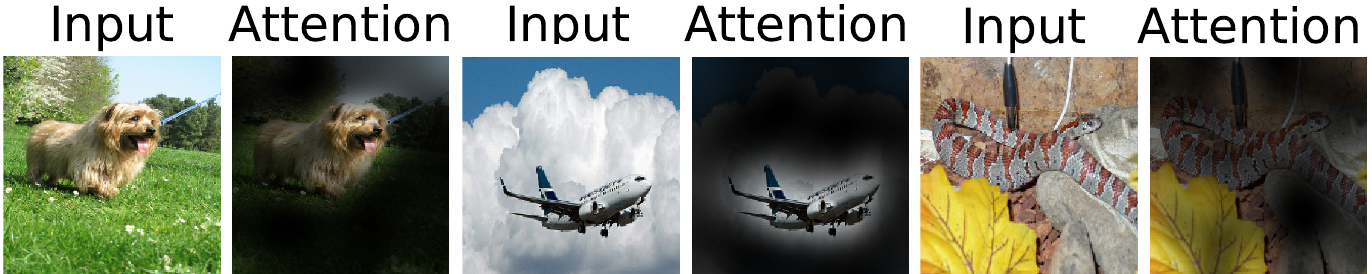
\includegraphics[width=\textwidth]{pictures/vit-attention2}\\
    \caption[Examples of Attention in Vision Transformers]{Representative examples of attention from the output token to the input space of a vision transformer. Figure and caption from~\autocite{Dosovitskiy2021}.}
    \label{fig:vit-attention}
\end{figure}

\begin{figure}[htb]
    \centering
    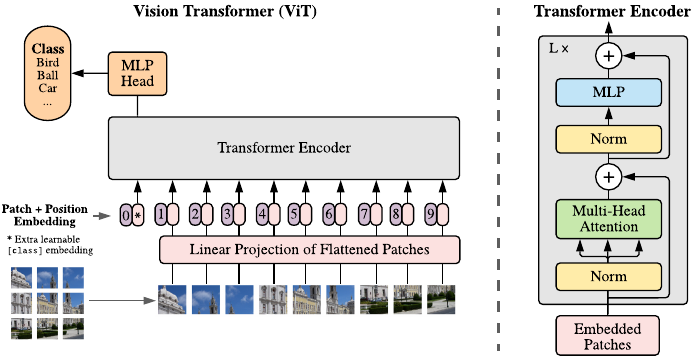
\includegraphics[width=\textwidth]{pictures/vit}\\
    \caption[Vision Transformer Model Structure]{Transformer model overview. An image is split into fixed-size patches, each of them is linearly embedded, the position embeddings are added, and the resulting sequence of vectors fed to a standard transformer encoder. In order to perform classification, an extra learnable ``classification token'' is added to the sequence. Figure and caption from~\autocite{Dosovitskiy2021}.}
    \label{fig:vit}
\end{figure}



% what ViTs can do:
The self-attention mechanism allows the vision transformer to integrate information from across the whole image in all layers, meaning that the receptive field is broad.
This is in contrast to convolutional neural networks, which do tend to have more narrow receptive fields (due to how the convolution algorithm works).
Additionally, transformers are still able to have smaller attention distances in the lower layer, meaning they can resolve local features well, too.
Overall, it was found, that the model attends to image regions that are semantically relevant, as seen in~\autoref{fig:vit-attention}.~\autocite{Dosovitskiy2021}

As mentioned before, for image classification only the classification token is considered, all other features are dropped.
%Transition to unsupervised segmentation
However, as it can be seen in the attention maps, these features contain semantic information about the image, and thus can be used for semantic segmentation~\autocite{Dosovitskiy2021}.
Thus, shortly after the vision transformer was introduced for image classification, algorithms were introduced that utilise these features for image segmentation tasks, for example by adding a projection head, that clusters the features~\autocite{Caron2021}.
It was even found, that features learned in an unsupervised fashion do contain even more relevant information, which can be used for clustering to generate a segmentation map of the input image~\autocite{Caron2021}.

 \subsubsection{Unsupervised Vision Transformer DINO}
% DINO - interpreting feature/attention maps, but make it self-supervised
Features learned in an unsupervised way often provide a richer signal than supervised features, since limiting the training to predefined concepts (for example to classification categories) reduces the rich visual information an image contains~\autocite{Caron2021}.
With unsupervised learning, information of an image assigned to another category might be utilised to build meaningful representations of that category or even other categories or semantic concepts.
%For example, learning representations of sky, even though that was not the intention of detecting street signs, might be helpful to figure out a scene.

In 2021, \citeauthor{Caron2021} set a new state-of-the-art for unsupervised segmentation algorithms with an algorithm called \gls{dino}\footnote{Knowledge distillation is a learning paradigm, where a student network is trained to match a teacher network~\autocite{Caron2021}.}.
It uses a pair of vision transformers as student and teacher networks ($g_{\theta_s}$ and $g_{\theta_t}$) to distill\footnote{Other networks can be used as backbone, but vision transformers were found to perform exceptionally well~\autocite{Caron2021}.} the image features (\autoref{fig:dino-structure})~\autocite{Caron2021}.

\begin{figure}[htb]
    \centering
    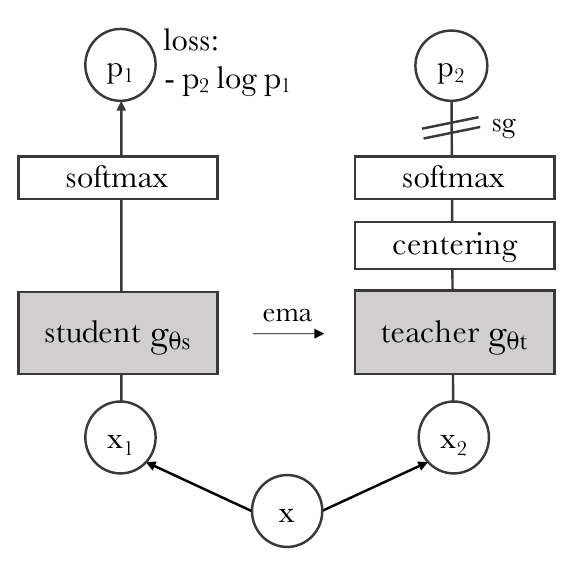
\includegraphics[width=0.55\textwidth]{pictures/dino-structure}\\
    \caption[Structure of DINO]{Self-distillation with no labels. Illustration of DINO in the case of one single pair of views ($x_1$ , $x_2$ ) for simplicity. The model passes two different random transformations of an input image to the student and teacher networks. Both networks have the same architecture but different parameters. The output of the teacher network is centered with a mean computed over the batch. Each network outputs a $k$ dimensional feature that is normalized with a temperature softmax over the feature dimension. Their similarity is then measured with a cross-entropy loss. We apply a stop-gradient (sg) operator on the teacher to propagate gradients only through the student. The teacher parameters are updated with an exponential moving average (ema) of the student parameters. Figure and caption from~\autocite{Caron2021}.}.
    \label{fig:dino-structure}
\end{figure}

The forward pass in each of these two network is calculated as followed, (where $\tau_s > 0$ is a temperature parameter to control sharpness of the output distribution):
\begin{equation}
    P_s(x)^{(i)} = \frac{exp(g_{\theta_s}(x)^{(i)} / \tau_s)}{exp(\sum^K_{k=1}g_{\theta_s}(x)^{(k)} / \tau_s)}
    \label{eq:forward-pass}
\end{equation}

The example given is for the student network, but since student and teacher architecture are the same, output of the teacher will be calculated analogously.

%backwardspass
The loss function of the student network is the cross-entropy loss between teacher and student, while the weight update for the teacher is done by an exponential moving average from the student's weights (also known as momentum encoder)~\autocite{Caron2021}.
For training, each network gets different crops of the same image (taken from a set of views $V$ of the image), but only global crops $x^g_i$ (comprising more than half the input image) are passed to the teacher, while the student gets local and global crops, to encourage a local-to-global correspondence~\autocite{Caron2021}.
Thus, the loss function in the student to be minimised is  (with $H$ being the cross entropy loss $H(a,b) = -a \log(b)$):
\begin{equation}
    \min_{\theta_s} \sum_{x \in \{x^g_1, x^g_2\}} \sum_{\substack{x' \in V \\ x' \neq x}} H(P_t(x), P_s(x'))
    \label{eq:loss-with-crops}
\end{equation}
The weight update in the teacher will be done by an exponential moving average from the student's weights.
Additionally, to avoid collapse in the teacher network, centering and sharpening is used on the output before applying the softmax function.\footnote{There were found two forms of collapse: regardless of the input, the model output is either uniform along all the dimensions or dominated by one dimension.}
Centering was found to hinder one dimension to dominate, but may encourage collapse to a uniform distribution.
Sharpening has an opposite effect.
So, combining both was found to stabilise the model.~\autocite{Caron2021}

% results of DINO
When evaluating this set-up, the authors found that different segmentation heads did attend to different semantic regions of an image even when they were occluded, meaning they were specialised to detect certain semantic patterns~\autocite{Caron2021}.
Additionally, the self-attention maps associated with a classification token\footnote{The name of this now unsupervised token was maintained for consistency with previous works.} showed that the architecture automatically learned class-specific features, as seen in~\autoref{fig:dino-attentionmaps}.
Even though neither the training objective nor the architecture were designed for such dense tasks, the self-attention maps of the vision transformer could be used straight away as segmentation maps, as seen in~\autoref{fig:dino-attentionmaps}~\autocite{Caron2021}.
This underlines the huge potential the self-attention maps of an unsupervised Vision Transformer have.

Not long after \gls{dino} was published, an architecture followed which expanded \gls{dino} by adding an energy-based graph optimisation to better generate segmentation masks from the self-attention maps~\autocite{Hamilton2022}.
This architecture is called \glsfirst{stego}.

\begin{figure}[htb]
    \centering
    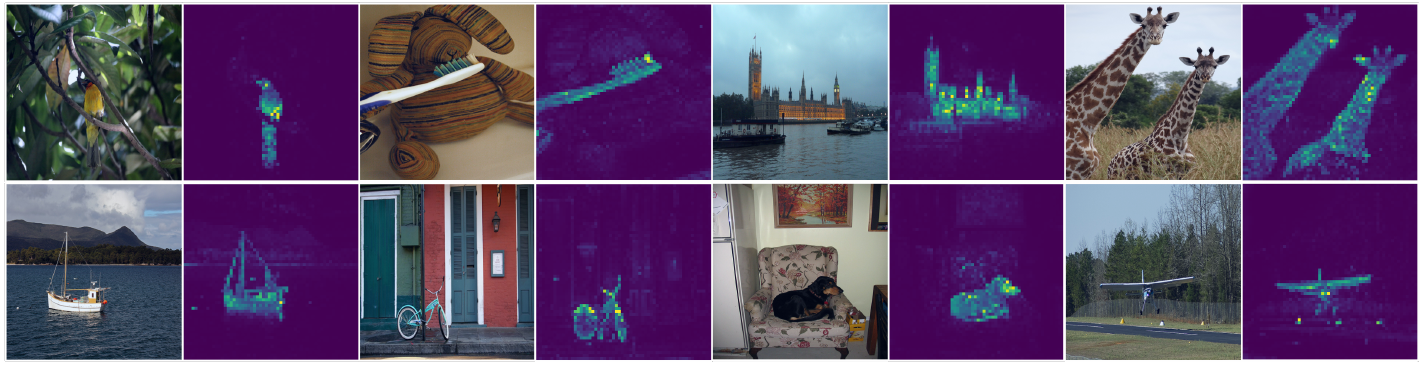
\includegraphics[width=\textwidth]{pictures/dino-attentionmaps}\\
    \caption[Self-attention Maps of DINO]{Self-attention from a vision transformer with 8 × 8 patches trained with no supervision. We look at the self-attention of the classification token on the heads of the last layer. This token is not attached to any label nor supervision. These maps show that the model automatically learns class-specific features leading to unsupervised object segmentations. Figure and caption from~\autocite{Caron2021}.}
    \label{fig:dino-attentionmaps}
\end{figure}

\section{Unsupervised Segmentation with STEGO}\label{sec:stego}
Shortly after the first unsupervised vision transformer was introduced~\autocite{Caron2021}, an architecture utilising the resulting attention maps for segmentation was presented~\autocite{Hamilton2022}.
This \glsfirst{stego} exploits the already dense and semantically consistent features produced by unsupervised architectures, and optimises them to form distinct clusters~\autocite{Hamilton2022}.

\subsection{Model Structure}
%overview components
\gls{stego} adds a light-weight segmentation head to the chosen backbone architecture to transform the features into meaningful segmentation maps.
The segmentation head consists of a feedforward neural network with \gls{relu} activation function to refine features obtained from the backbone, a clustering function to combine these features into labels\footnote{When ground truth labels are provided during training, an additional network is trained, which is a linear projection of the distilled segmentation features to the class labels using the cross-entropy loss.
Note, that this is only used to evaluate the final segmentation results! However, it will also provide segmentations for predictions, but during training of \gls{stego} no labels are used.}, and a fully connected conditional random field optimisation to ``sharpen'' these labels and improve spatial resolution further by aligning the predictions to the image edges.~\autocite{Hamilton2022}

The utilised loss function is an energy-based graph model, hence the name of \gls{stego}.
The backbone is frozen and not trained in any capacity by \gls{stego}, which is why the training time is relatively short~\autocite{Hamilton2022}.
\gls{stego} was found to perform best, when using the \gls{dino} backbone~\autocite{Hamilton2022}, which is plausible since \gls{dino} already provides very promising attention maps~\autocite{Caron2021}.
However, it can be easily adjusted to use other backbones, once more promising candidates become available.

Since \gls{stego} scales down all images to a user selected resolution, an additional performance boost was found, when images were ``five-cropped'' before training, meaning the original images are cropped into five separate regions, one of each corner and one center-cropped.
This way, more details can be utilised during training for each picture.~\autocite{Hamilton2022}

\subsection{Loss Function}\label{subsec:stego-loss-function}
%details on procedure: segmentation head loss function
In the segmentation head, the features provided by the backbone are refined using a novel contrastive loss function that optimises the feature vectors to yield very good semantic segmentation when they are clustered.
As all contrastive loss functions, it relies on an instance discrimination task, where positive view pairs (crops or distortions from same or similar images) are compared with negative view pairs (from different images).
This is done by utilising the correspondence between feature vectors and semantic segmentation, as indicated by the self-segmentation maps.~\autocite{Hamilton2022}

\parbox{\textwidth}{The feature correspondence tensor, a similarity measurement between two locations ($h,w$ and $i,j$) of two images $f$ and $g$, is defined as:}

\begin{equation}
    F_{hwij} = \sum_c \frac{f_{chw} g_{cij}}{|f_{hw}| |g_{ij}|}  
    \label{eq:correspondence}
\end{equation}
This represents the cosine similarity between the feature at spatial position $h,w$ of feature tensor $f$ and position $i,j$ of feature tensor $g$.
The chanel dimension is given by $c$.
Working through all positions of these tensors, a full picture of the correspondence of these two images (according to their feature vectors) can be calculated, as visualised in~\autoref{fig:stego-feature-correspondence}.~\autocite{Hamilton2022}

\begin{figure}[!htb]
    \centering
    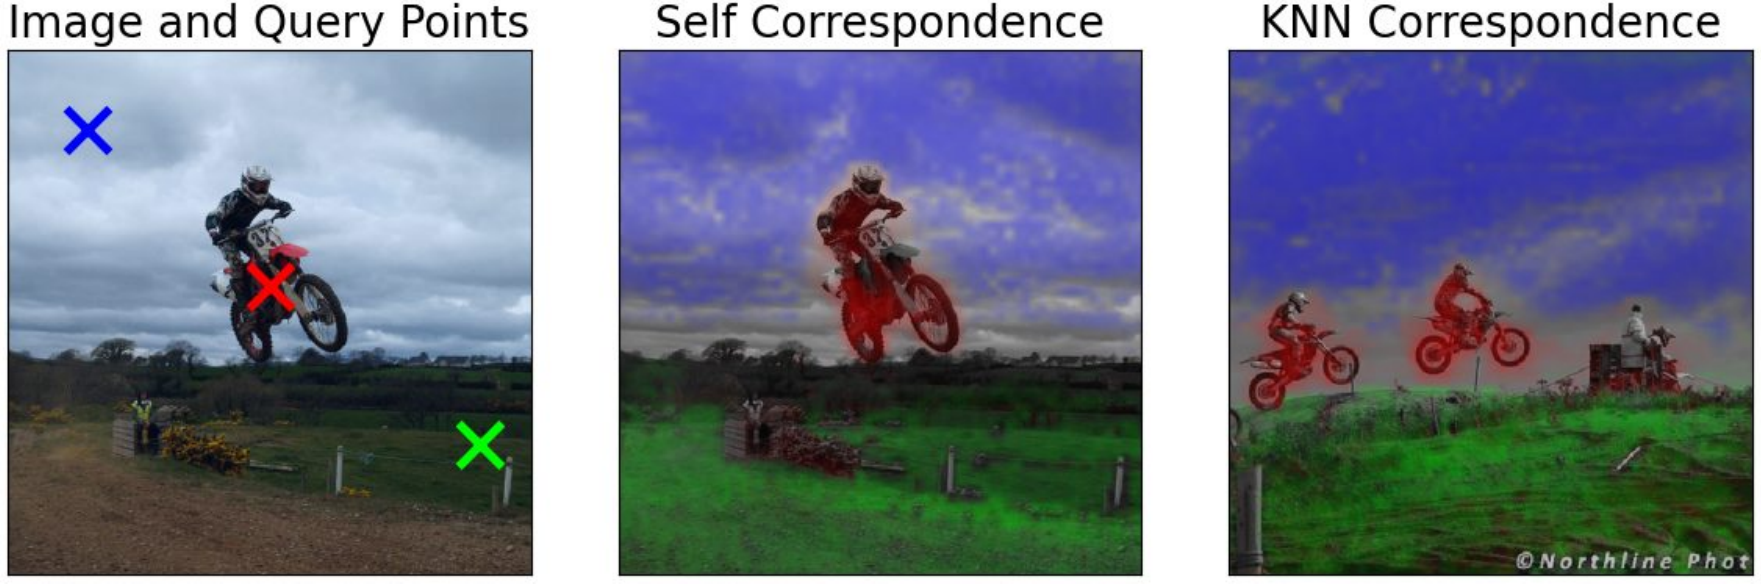
\includegraphics[width=\textwidth]{pictures/stego-feature-correspondence}\\
    \caption[Feature Correspondence of Two Images]{Feature correspondences from DINO. Correspondences between the source image (left) and the target images (middle and right) are plotted over the target images in the respective color of the source point (crosses in the left image). Feature correspondences can highlight key aspects of shared semantics within a single image (middle) and across similar images such as one of the k nearest neighbours (KNNs) (right). Figure and caption from~\autocite{Hamilton2022}.}
    \label{fig:stego-feature-correspondence}
\end{figure}

The feature correspondence signal $F_{hwij}$ can be used for high quality semantic segmentation by comparing it with the segmentation correspondence tensor $S_{hwij}$, which is calculated respectively (see~\autoref{eq:correspondence}).
The loss function aims at pushing the segmentation tensors together, when the feature tensors were found to have stronger correlation.
Additionally, zero clamping and spatial centering is applied, to hinder collapse and to balance the learning signal for small objects respectively.~\autocite{Hamilton2022}

The correspondence loss function of two images ($x$, $y$) thus is:
\begin{equation}
    L_{corr}(x,y,b) = -\sum_{hwij}\left(\underbrace{\left(F_{hwij} -\frac{1}{IJ} \sum_{i'j'}F_{hwi'j'}\right)}_{\substack{\text{spacial centered} \\ \text{correspondence loss}}}- b\right) {} \underbrace{max(S_{hwij}, 0)}_{\substack{\text{zero clamped}\\\text{segmentation} \\ \text{correspondence}}}
    \label{eq:corr-loss}
\end{equation}
Where $b$ is a negative pressure to again avoid collapse, $h,w$ are positions of image $x$ and $i,j$ positions of image $y$.
$I,J$ represent spatial dimensions.
This loss function will administer a repulsive or attractive force on the segmentation features, proportional on their feature correspondence.
The function $L_{corr}$ was shown to be a Potts model, an energy-based graph optimisation model, hence the name of \gls{stego}.~\autocite{Hamilton2022}

\gls{stego} uses three instances of the correspondence loss as final loss function to train the segmentation head: one between the image and itself, one between the image and one of its k-nearest neighbours\footnote{It was found by the authors that selecting from the seven nearest neighbours yields good results.} (both of these exerting an attractive force), and one instance between the image and five random other images, exerting a repulsive force.
To balance the negative and positive signals, weight parameters $\lambda$ are used.~\autocite{Hamilton2022}

The loss function optimised in the segmentation head thus is:
\begin{equation}
\begin{aligned}    
    L = {} & \lambda_{self}L_{corr}(x,x,b_{self}) \\
        & + \lambda_{knn}L_{corr}(x,x^{knn},b_{knn}) \\
        & + \lambda_{self}L_{rand}(x,x^{rand},b_{rand})
    \label{eq:stego-loss}
\end{aligned}
\end{equation}

In practice the authors recommend a ratio of $\lambda_{self} \approx \lambda_{knn} \approx 2 \lambda_{random}$, while the $b$s need to be tuned on a per-data-set basis, usually optimised to balance the mean knn feature similarity at $\approx 0.3$ and mean random similarity at $\approx 0.0$\footnote{This can be achieved by monitoring the provided TensorBoard (especially the variables \posinter and \neginter).}. % mean self similarity should always be at 1? depends on corpping and dataset...
However, as seen in the appendix of the paper, other weight relations were also found beneficial for different data sets.~\autocite{Hamilton2022}

\subsection{Potential and Problems}
%evaluation (calculating precision and recall)
%Since the feature correspondence is strongly correlated with the true label co-occurrence tensor $LCo$, it can be used to evaluate feature compatibility in regard to semantic segmentation using, by predicting the label co-occurrence.
%By examining how well the feature correspondence $F$ can predict the label co-occurrence $LCo$ a measure on the compatibility of the features withe the ground truth labels is found (precision and recall).
%\begin{equation}
%    LCo_{hwij} =  \begin{cases}
%                      1, & \text{if~} l_{hw} = k_{ij} \\
%                      0, & \text{if~} l_{hw} \neq k_{ij}]
%                \end{cases}
%    \label{eq:label-coocurrence}
%\end{equation}
%If two ground truth labels $l$ and $k$ are the same, label co-occurrence is 1, else label co-occurrence is 0.

% performance is very good
The authors found, that this feature distillation process did in fact significantly improve the performance in comparison to directly clustering the unmodified features the backbone provides.
In the best scenario, \gls{stego} improved the prior state-of-the-art by 9 to 14~points on the \gls{miou}~\autocite{Hamilton2022}.
Additionally, training is very fast, since the backbone is frozen with pre-trained weights provided by \gls{dino}, and only the lightweight segmentation head is trained~\autocite{Hamilton2022}.

By providing extensive configuration files, the authors allow users of \gls{stego} to adjust the network to their specific use cases.
For example, resolution and batch size can be adjusted to the image size in the train set, and different cropping methods are provided to pre-process images to account for more details in the pictures.\footnote{With the data sets used in the paper, five cropping (as explained before) was found most beneficial, but a random cropping utility is available too, which might be beneficial for different data sets.~\autocite{Ji2019}}
For training, different (pre-trained) backbones can be selected, and even completely new backbones can be integrated, once more promising candidates become available or are trained on a specific data set.~\autocite{Hamilton2022}

Additionally, training can be done with extra clusters to enable overclustering~\autocite{Hamilton2022}.
Overclustering refers to the practice of clustering with more clusters than ground truth labels.
It was theorised by~\autocite{VanGansbeke2021}, that improvement through overclustering could be attributed to the fact that pixels of the same (or visually similar) objects are found in local neighborhoods in the embedding space of models.
More practically, it can also be assumed, that allowing multiple clusters for a ground truth label, that encompasses different textures, can increase overall performance.

% (transition) but some problems when used for scientific data
However, \gls{stego} (as well as its backbone) was adapted for 2D RGB photographs~\autocite{Hamilton2022}.
This means for training 3D high-resolution grey value images, as often found in scientific imaging, some adjustments need to be made.
Additionally, it was found, that some functionalities provided in the code base did not work as intended, and needed fixing~\autocite{mhamilton7232022}.
Overall, this means, the method was not yet ready to use when downloaded from GitHub~\autocite{mhamilton7232022}, and some adaptions and corrections needed to be made before using it.

\section{Adapting STEGO for Scientific Images}\label{sec:adapting-stego}
As mentioned before, \gls{stego} needed some adaptions to be used with 3D high-resolution scientific images.
This comprised correcting and refactoring the code to make it executable, setting all the configuration variables to the optimal values as found by the authors or according to the data set used for training, and also adapting \gls{stego} to be used with high-resolution grey value images, since the expected inputs were 2D RGB color photographs.~\autocite{Hamilton2022}


\subsection{Code Refactoring and Corrections}
%configuration files
Since the code base of \gls{stego} was very much the raw project, which contains all experiments presented in~\autocite{Hamilton2022}, there were a lot of configuration variables present. 
For these the optimal values often have been already found by the authors, so they were not needed anymore or best set to a predefined value.
Moreover, the provided configuration files were often not used consistently in the executable scripts.
Frequently, the configuration parameters from the configuration files were overwritten with hardcoded values in the executable files.
Overall, these problems could be solved by replacing all the hardcoded parameters with parameters from the configuration file first and then investigating which configuration variable belonged to which part of the experiments mentioned in the paper (since they were not documented at all).
Finally, the configuration file structure was adapted to a hierarchy, so it was easier to distinguish between parameters to define the backbone, parameters to control training, and parameters for selected data sets.

% fixes during training
The training procedure did only work for the provided example datasets and not for own datasets (directory datasets), since during the validation, label names are required, which were again hardcoded for the example datasets, but of course not available for directory datasets.
This was solved by adding a labels parameter to the configuration file, which is read when own datasets are trained.
Calculation of the nearest neighbours of an image was changed to read the images in the given resolution, instead of using the hardcoded (down-scaled) size, since it is expected that better matching neighbours will be found.

% fixes during validation
Other fixes were needed during validation when creating diagnostic pictures, since the label number was calculated incorrectly when extra clusters were used.
Additionally, the label tensor made during training needed squeezing in order to be passed to the plotting function during validation (so some example predictions can be plotted to illustrate the training progress via \tensorboard).
Lastly, loading of the validation images was changed to always load the original validation images (of the un-cropped dataset), since loading the down-scaled images would provide only very weak evidence on model improvement.
Additionally, resolution and batch size of the validation set was adapted to be selected independently of the train set, so the validation images can be interpreted easier. 

% `fixes' during evaluation
The evaluation procedure used by the authors focused on comparing \gls{stego} with the former state of the art for unsupervised segmentation (PiCIE~\autocite{Cho2021}), so new evaluation scripts were made to evaluate a trained model based on a test set.\footnote{With the new evaluation script, evaluations can be done by running the model on a test set belonging to the data set the model was trained on or by giving a path to the image and ground truth folder to be used for evaluation.}
During evaluation, \gls{miou} and accuracy for the test set are reported, as well as some diagnostic graphs, to show correlation between ground truth labels and predicted labels, as well as to display some example segmentations side by side with their ground truth and original image.

% cosmetic corrections (refactoring)
Additionally, some non-functional alterations were made:
\begin{itemize}
    %\item Repaired issue with the evaluation script not showing a progress bar by fixing multiprocessing.
    \item For better adaptability and easier way of training on different data sets, the configuration file structure was adjusted, so that for every script, the base configurations are collected in one configuration file, while all data set specific configurations are collected in a separate file, which is selected via the command line for each training separately.
    \item The output directories were changed to depend on the output path given in the configuration, instead of saving everything in the code folder.
    \item For better comprehension and clearer view on what is happening in the code, the full configurations are no longer passed between scripts, only the relevant variables extracted from the configuration will be passed.
    \item The code was also adjusted to get rid of warnings of future deprecations, since the provided conda environment specified some very particular, but often older versions for packages.\footnote{As it was found that updating \gls{stego} to other Python versions leads to problems during training, it was decided to not change the suggested conda environment.}
    Note, that not all warnings have been resolved.
\end{itemize} 

%Things that should be changed, but weren't:
Due to time constraints, some issues have not been addressed, since they do not influence results, but mainly user experience.
For a full list see~\autoref{subsec:stego-persisting-issued}.


\subsection{Adaption to High-resolution Grey Value Images}
\gls{stego} was designed with photographs in mind.
Thus, some adaptions needed to be made to use it with scientific images, mainly to adjust the normalisation scheme to grey values, load high-resolution images and handle 3D images.
In the following, these changes are documented, always in relation to the original architecture~\autocite{Hamilton2022}.

The more simple adaption concerned the normalisation scheme during preprocessing, when a pixel value normalisation for each channel was done, based on the mean and standard deviation of the ImageNet data set\footnote{https://www.image-net.org/ (visited 15/02/2023)}.
The different normalisation of the three RGB channels was of course not appropriate for images that represent grey values.
Thus, in the configurations file used for training, a flag was added to indicate if images are grey values and in \gls{stego}, a normalisation function based on the grey value of ImageNet pictures was added.

Another problem was the scaling \gls{stego} applies when loading images.
Since often images could not be loaded at full resolution, all images were scaled to the user-defined resolution.
For scientific data, this means a lot of the cumbersome earned and probably relevant details would be lost.
Thus, a second flag was added in the configuration file to switch between down-scaling and center-cropping the loaded images to size.
Of course, this way some data is still lost, but instead of loosing overall details, now the borders of the images are missing, which are often not the regions of interest.
Overall, establishing the possibility to crop instead of scale means, that in combination with five-cropping and selecting an appropriate resolution, the maximal amount of relevant details of the images can be utilised with \gls{stego}.

For a more fine-grained evaluation, \gls{stego} was also adapted, to display the label-wise \gls{iou} (additional to the mean over labels) in the \tensorboard to better understand how individual labels perform.
This change did not alter the architecture significantly, since these values could be simply extracted before the mean was calculated.


\gls{stego} originally was developed to train and predict 2D photographs.
To use it with 3D data, the volumes need to be sliced into a stack of 2D images (and reassembled later on).
Therefore, a data converter was designed, which converts the in-house data sets to the required format.
However, data conversion is done separately from \gls{stego} and thus not part of this project.

\begin{figure}[!htb]
    \centering
    \vspace{1em}
    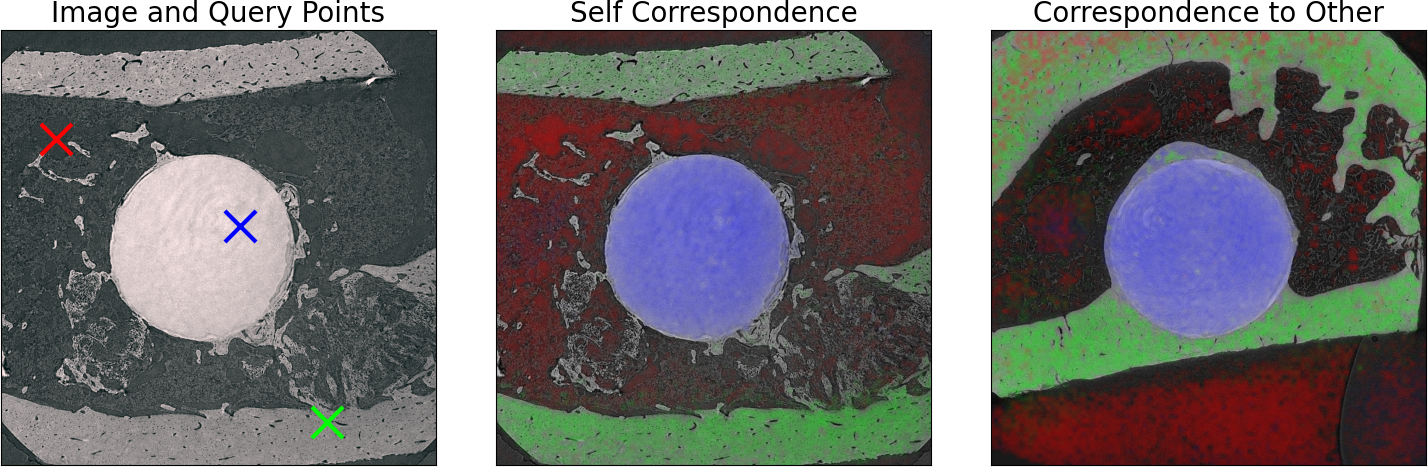
\includegraphics[width=\textwidth]{pictures/correspondencemaps_syn030-slice300_113724Mg10-slice500}\\
    \caption[Feature Correspondence for SRµCT Images]{Feature correspondences maps for SRµCT images derived from the DINO-backbone of \gls{stego}. Correspondences for selected points (marked with x) are plotted over the same (middle) and another target image (right) in the respective color of the source point.}
    \label{fig:correspondencemap-screws}
\end{figure}

It was decided to use the frozen backbone that was trained on photographs too, since investigating exemplary attention maps showed, that this backbone is already able to indicate correspondences from \gls{srmct} images, as seen in~\autoref{fig:correspondencemap-screws}.
This can be interpreted as a form of transfer learning~\autocite{Litjens2017}, which yields promising results in some cases, as networks trained exactly on this data set have been found to yield good results when used with medical images as well (for an overview on performance of transfer learning, see~\autocite{Cheplygina2019}).











\section{Evaluating the Adapted STEGO}\label{sec:proof-of-concept}
% experiments introduction
In a first step, the pre-trained models shipped with \gls{stego} were used to predict a selected data set (screws data set).
This could hint at a general transferability of models and was also used as base-line for comparisons with the second experiment, where \gls{stego} was trained on the screws data set with different cropping regimes.
Since \gls{stego}s loss function leverages the signal of similar and dissimilar features in images, and most scientific imaging experiments reproduce scans of the same object over and over again, trainings were done with different cropping regimes to artificially increase heterogeneity between slices.


\subsection{Methods}
In the following, an overview on the used methods is given.
The data set used for the experiments is introduced, and the experiments are explained.

\subsubsection{Data Set}
Both experiments were run on an in-house data set (screws data set), originally gathered to investigate how biodegradable bone implants (screws) are absorbed by the body after implantation~(\autoref{fig:screws-example}).
The aim of the segmentation was to differentiate between the labels \formatLabel{bone, degraded screw, screw} and \formatLabel{background} (also containing soft tissues).
A ground truth segmentation was available for all samples used.
The particular challenge of this data set was the label \formatLabel{degraded screw}, which was scarce in comparison to the other labels, so there was a pronounced imbalance between labels.
Additionally, pixels belonging to this label often had very similar pixel values and also textures as the \formatLabel{screw} label.
So overall, it was mostly distinguished through its borders, and did not consist of homogenous pixels.
This data set has been used before with a supervised learning approach~\autocite{Baltruschat2021}, so a direct comparison of the model performance can be made.

The data set consisted of 17 3D high resolution \gls{srmct} scans of magnesium alloy screws in bone, that were either made at the P05 imaging beamline at \gls{desy} or at the Diamond Manchester Imaging Branchline I13-2.
Afterwards, volumes were resampled with bi-linear interpolation to a fixed voxel-size of 5~µm, clipped to a dynamic range of 0.5 and 99.9~\% and normalised, so grey-values are in the range [0,1].
Each volume was cropped to a size of $1200 \times 1200 \times 1000$~px.
The ground truth of the samples was obtained via a time-consuming semi-automatic workflow, based on watershed segmentation.
14 of the semi-automatically segmented samples were used as train set (of which three were used for validation in each fold during five-fold cross-validation).
The remaining three samples were used for predictions only\footnote{Predicted volumes were: 113734HQMg5, syn009HQ, and 113729HQMg5.}.
For these three volumes, high quality segmentations were available done by an expert, who manually corrected the semi-automatic segmentation.
For more details on beam intensity, image reconstruction, and ground truth workflow see~\autocite{Baltruschat2021}.

\begin{figure}[!htb]
    \centering
    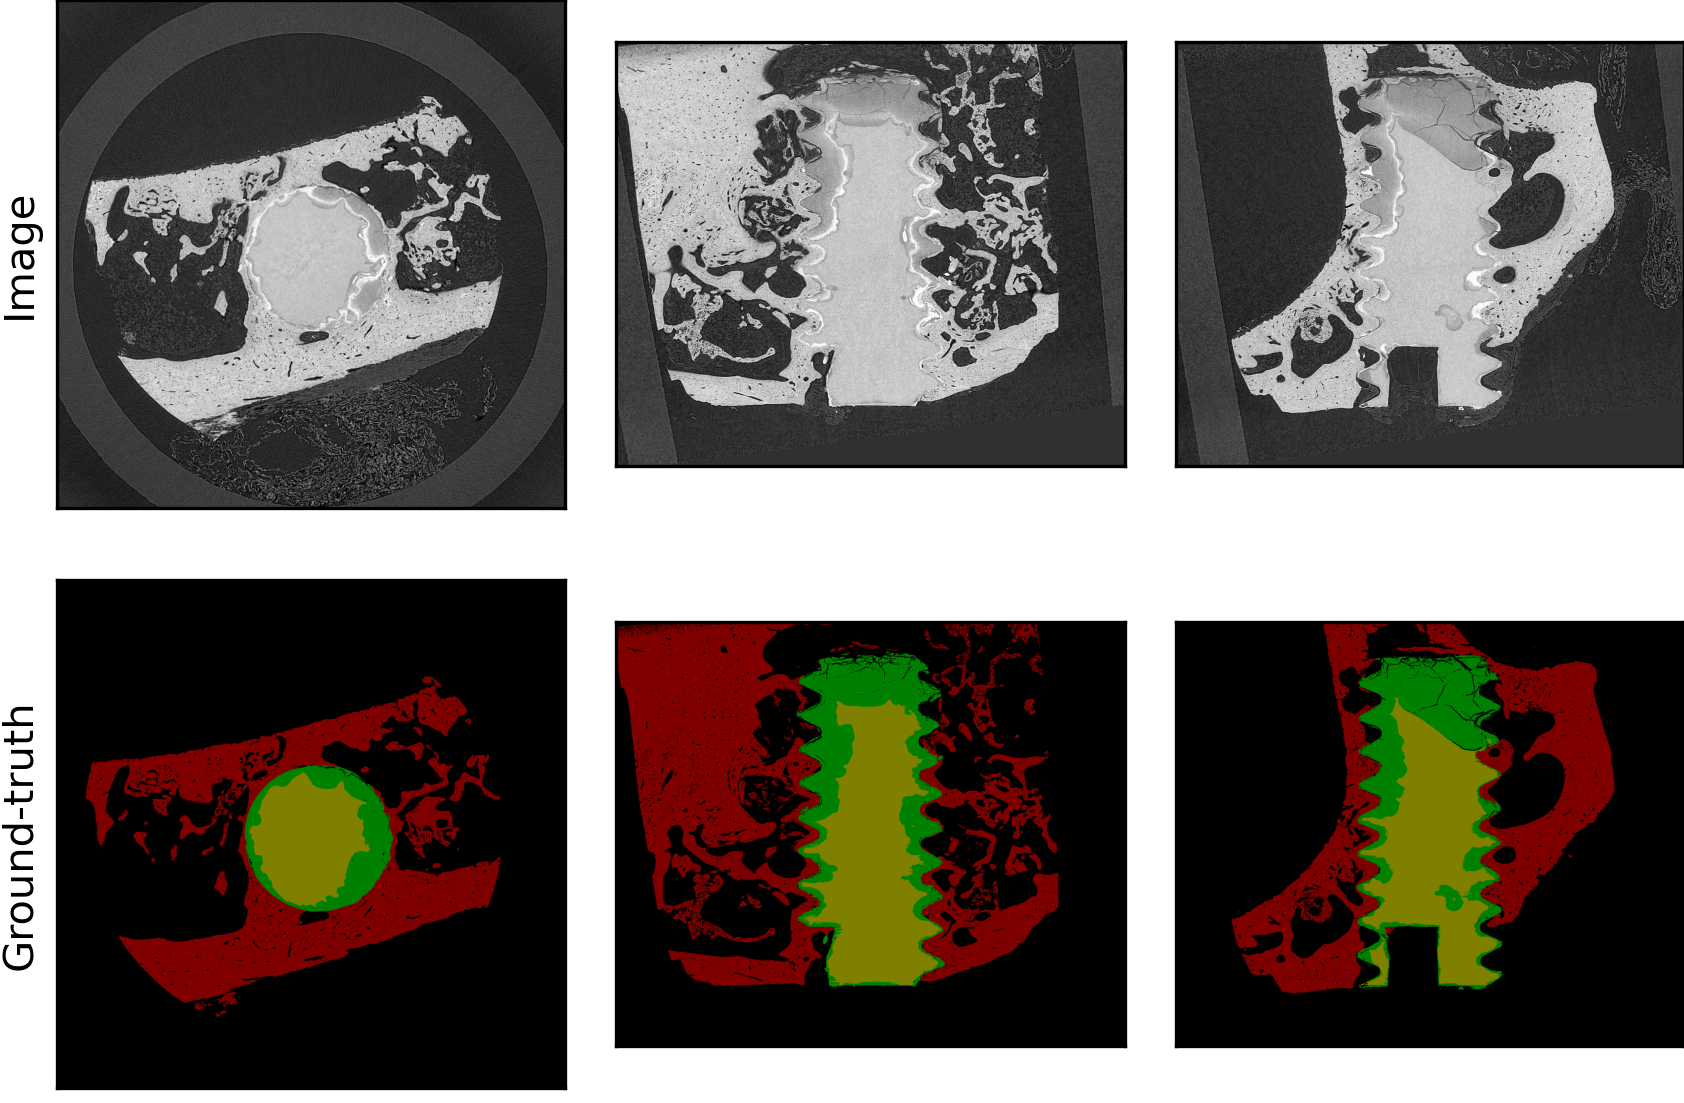
\includegraphics[width=\textwidth]{pictures/ExampleImageGroundtruth_syn009_slice500_allDirections}\\
    \caption[Example Images of Screws Data Set]{Example of images and ground truth segmentation of the screw data set. Slice 500 in every direction of volume syn009HQ is shown. The label color map is as follows: \formatLabel{background}: black, \formatLabel{bone}: red, \formatLabel{degraded screw}: green, \formatLabel{screw}: yellow.}
    \label{fig:screws-example}
\end{figure}

%\paragraph{Amber}
%The second data set used in the experiments consists of 19 \gls{srmct} image volumes of amber with arachnid inclusions.
% http://www.panarthropoda.de/sub/allgemeines/pseudoskorpioneen.php
%This data set was originally assembled to visualize the enclosed pseudoscorpions\footnote{Pseudoscorpions are a very old group of arachnids, resembling scorpions and reach sizes between 2 to 10~mm~\autocite{Harvey2002}.}
%Voxel-size was 2.4~µm, but image volumes vary in size, depending on size of the inclusion.
%The biggest volume is $1469 \times 1239 \times 1443~px$, the smallest $626 \times  348 \times  458~px$.
%By varying the slicing direction, the image slices could be brought to a minimal size of $626 \times 458~px$ and maximal size of $1239 \times 1443 px$.

% describe were images come from
%SRµCT images were obtained at \gls{desy}, at the storage ring PETRA III, Beamline P05.
%The attenuation contrast was conducted with an energy of 25~keV, the number of projections was 1200, and voxel size 2.4~µm.
%Scan time was about 2 hours for each scan.
%Projections were reconstructed to 32-bit floating point image stacks with the tomographic reconstruction algorithm ‘gridrec’.
%Ground truth segmentation of the scans was done manually for 12 of the 19 volumes in Amira (Thermo Scientific, 2016). % and took about 15 hours for each scan.
%First rough segmentation of the specimens was done via threshold selection, but completion had to be done manually.
%Especially bubbles and other impurities often had to be separated from the specimen manually slice by slice.

%\begin{figure}[!htb]
%    \centering
%    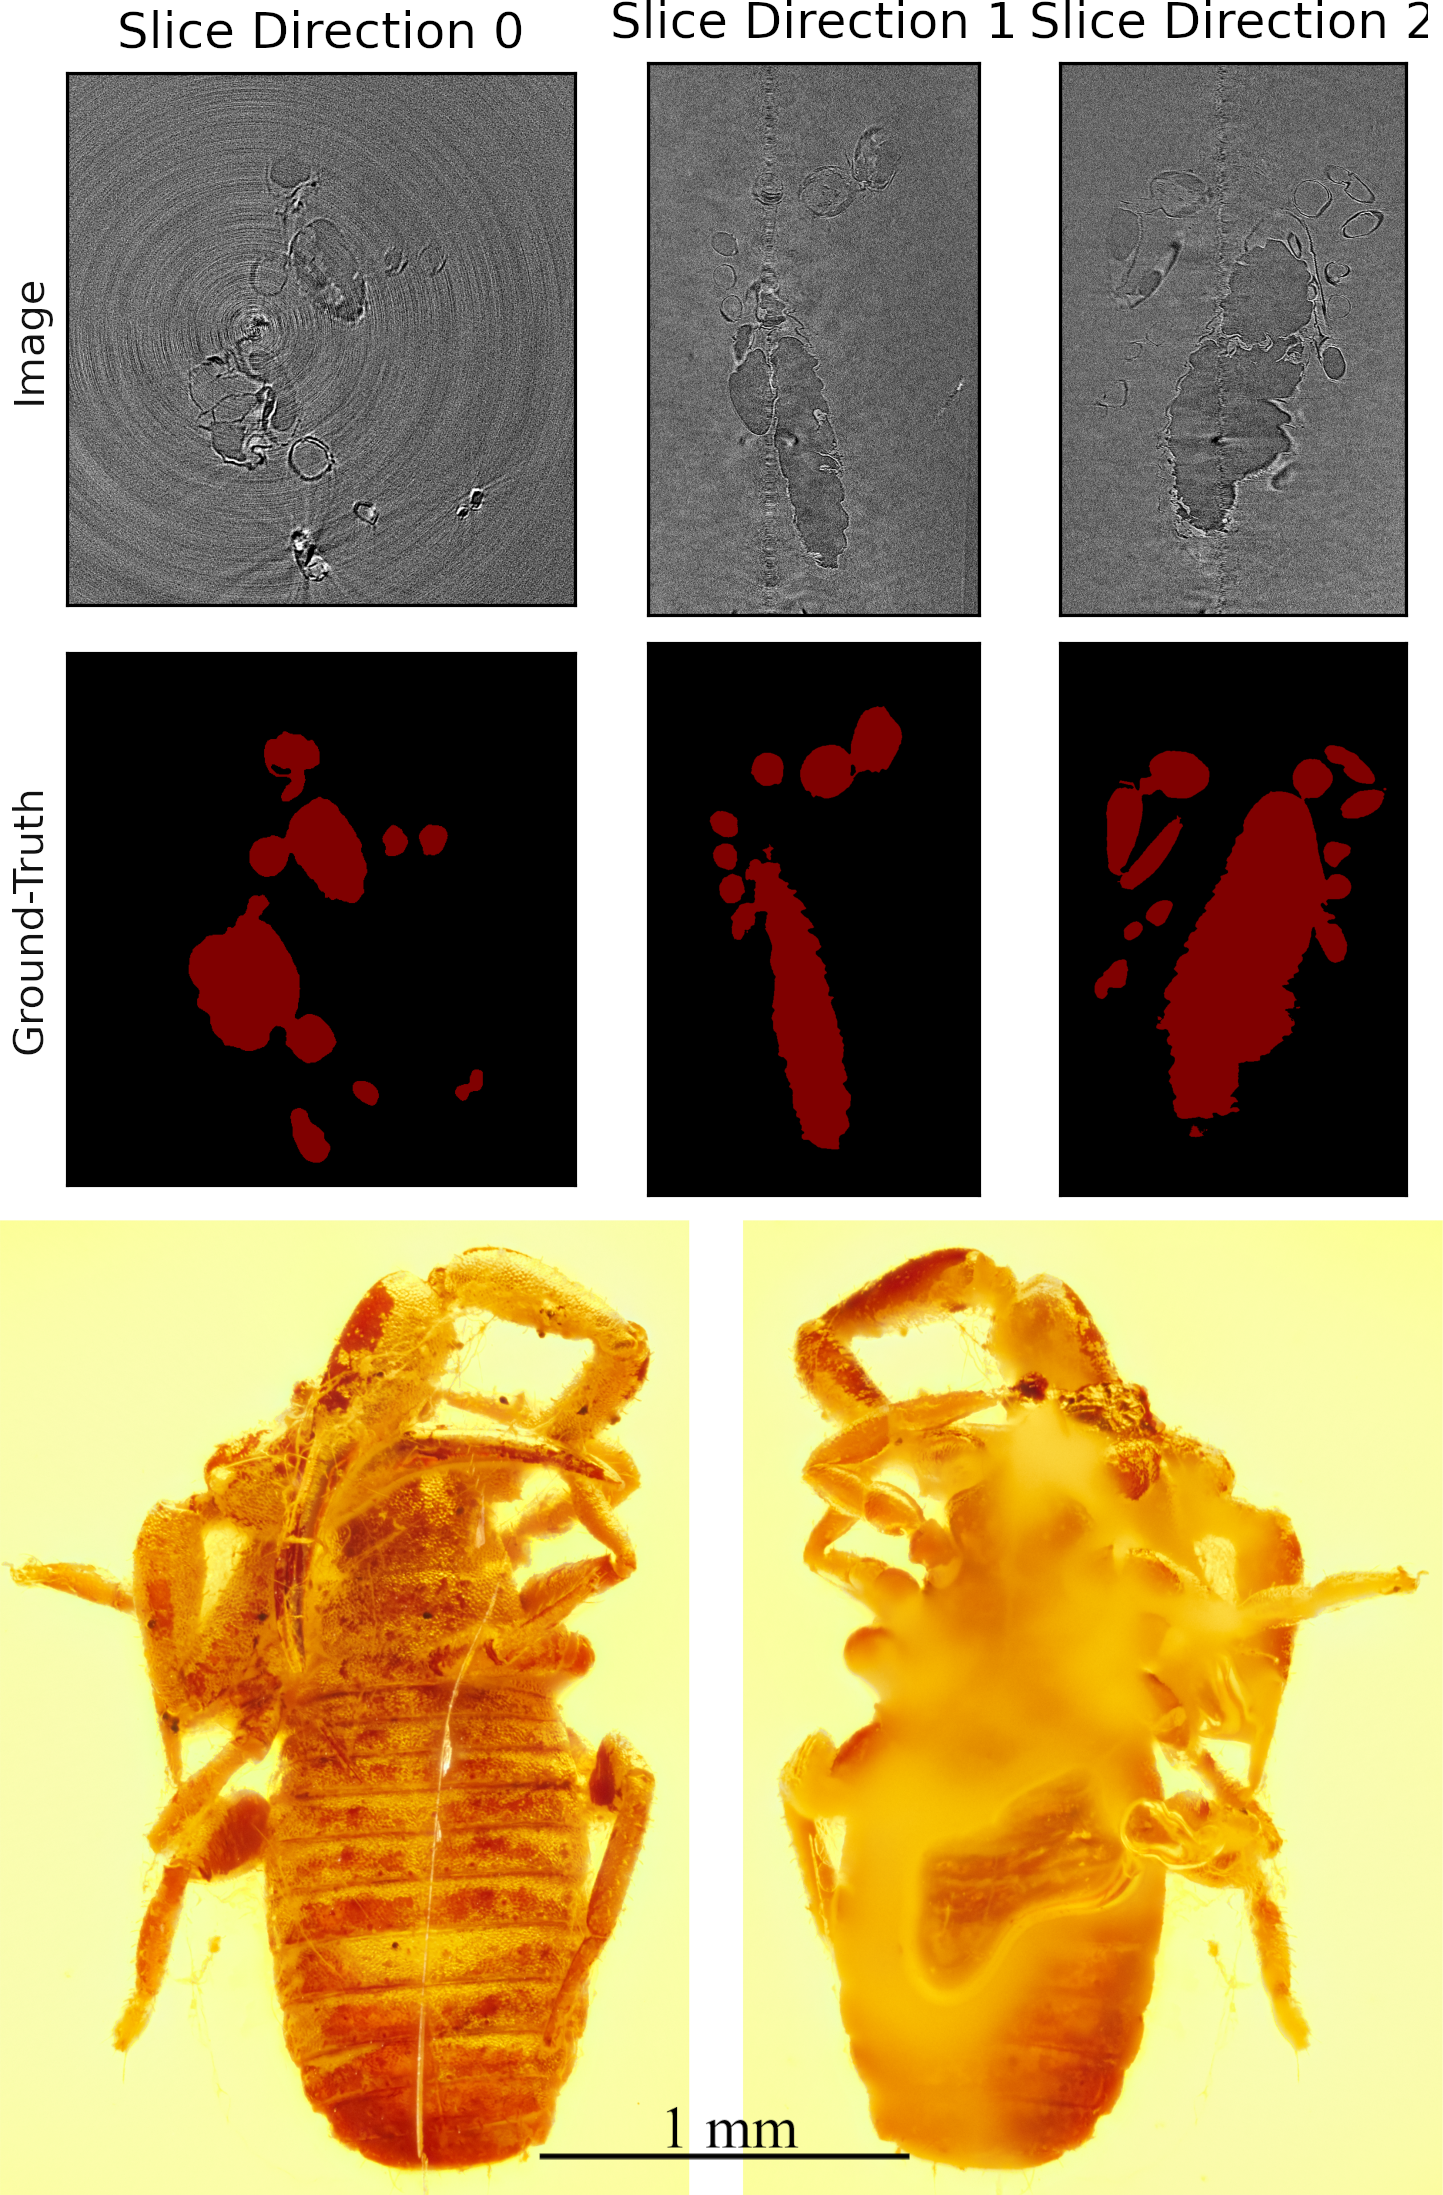
\includegraphics[width=0.95\textwidth]{pictures/Segmentation_Photo_PS-4}\\
%    \caption[Example Images and photograph of Amber Specimen]{Example of an amber specimen with image, ground truth and dorsal and ventral high resolution photograph. As seen part of the ventral side is hidden from visual inspection due to white emulsion leaked from the specimen and bubbles in the amber piece.}
%    \label{fig:amber-example}
%\end{figure}

%\paragraph{Mixed Data set}
%Both mentioned data sets (screws and amber) were combined into a mixed data set, with roughly the same number of images from amber and screws set.
%From the screw data set, which is much bigger than the amber set, 23.491~images were randomly selected from the five-cropped set (where image size nearly matches image size of the smallest amber slices), so the resulting mixed data set contained the same amount of images from the amber and screws set.
%Since the amber images were of variable sizes, the mixed data set should only be used center cropped to the smallest resolution ($458 \times 458~px$).
%This means loosing some information of lager amber images, and loosing some border pixels of the five-cropped screws images.
%However, since the amber data is just used to increase heterogeneity of the screws data set, and the aim of the data set is to enhance the screws predictions, not amber predictions, this should not be a problem.\footnote{Another option would have been to divide the bigger amber images in smaller slices to retain more of the amber information and adjust the number of screws images selected accordingly, but for simplicity this is not done here. Nevertheless, in future work, this should be investigated.}
%Because ground truth labels were not available for all amber volumes and the experiments designed for this data set aim at improving predictions of the screws, the train-validate-test-split of the mixed data set was done in a way that the validation and test sets match the screws data set. 
%Amber images were only added to the training set.
%To account for the five-fold cross validation, the amber images thus were partitioned into folds separately from the screws images and added to the training folds of the screws images.
%Slices belonging to the same volume were always kept in the same fold.
%Volumes were distributed between folds, so that every fold contains nearly the same number of slices.
%For the amber folds this means a slight variety of number of slices per fold: 4405, 4406, 4407, 4423, and 4381.
% 1. select x random images form five-fold screws trainset (all folds), to match number of amber pictures
% 2. make a five-fold cross validation of the selected screws images
% 3. partition amber into 5 folds of same size (keep volumes together) and add them to the screws train folds
% 4. copy test set of screws data set (since no changes here)

%\subsubsection{Experiments}
%To asses the capacity of the original \gls{stego}, and also to get a first feel for the potential of \gls{stego} for scientific data, in the first experiment the screws test data set was predicted with the pre-trained models \gls{stego} provides.
%Experiment two was designed to determine if and how training \gls{stego} on very homogenous data sets is yielding satisfactory results.
%This is done by using different cropping regimes, and hyper parameter combinations.

\subsubsection{Experiment 1: Predict with Provided Models}
To get a first feel for the capacity of \gls{stego}, the three volumes selected for predictions of the screws data set were predicted with the provided pre-trained models.
If the pre-trained models were found to predict the test data set quite well, this would hint at extraordinary transferability and generalisation capacity of \gls{stego}.


%used models
Three pre-trained models were provided by the authors of \gls{stego}.
A model trained on aerial photographs of Potsdam\footnote{\url{https://www.isprs.org/education/benchmarks/UrbanSemLab/2d-sem-label-Potsdam.aspx} (visited 15/02/2023)} resolving three (of the six original) classes, the COCO-Stuff\footnote{\url{https://github.com/nightrome/Cocostuff} (visited 15/02/2023)} model, which was trained on the COCO-Stuff data set and resolves 27 classes, and a model trained on the Cityscapes data set\footnote{\url{https://www.Cityscapes-dataset.com} (visited 15/02/2023)}, also resolving 27 classes.~\autocite{Hamilton2022}

%data sets of models
The Potsdam data set was released by ISPRS Commission WG II/4.
It consists of 38 aerial photographs of the city op Potsdam, with six categories to be differentiated (\formatLabel{impervious surface, building, low vegetation, tree, car, clutter}).
In the pre-trained \gls{stego} model, only the categories \formatLabel{roads and cars}, \formatLabel{buildings and clutter}, and \formatLabel{vegetation and trees} were used.
The COCO-Stuff data set augments the large-scale COCO (Common Objects in Context) data set with pixel-level stuff annotations.
Thus, semantic classes can be objects with well-defined shapes as in COCO (e.g.~\formatLabel{car, person}) or stuff (amorphous background regions, e.g.~\formatLabel{grass, sky}).
Cityscapes is a large-scale data set, that contains a diverse set of images of urban street scenes from 50 different cities.
Categories in the data set include: \formatLabel{person, bus, building, sidewalk, vegetation, tunnel} etc.
This means, there is some overlap in the categories between COCO-Stuff and Cityscapes.~\autocite{Hamilton2022}

% execution of experiment
%cropping vs scaling
Since the selected test data had a very high resolution, the images could not be loaded in full resolution.
Even with a batch size of one, computing nodes quickly run out of memory.
Therefore, images needed to be reduced, either scaled or center-cropped.
Since in \gls{srmct} minor details matter, images were cropped.
% experimenal set-up
So, the predictions were made on the center-cropped images (to $800 \times 800~px$) with each given model.
This means, a 200~pixels wide stripe was missing on each side of the original slide ($1200 \times 1200~px$ resolution).
Since the region of interest was centred in the images and this outer border mostly contained background (and some bone pixels), loosing the outer border was tolerable for this data set.
% evaluation of predictions
Predictions were evaluated using the Hungarian matching algorithm on the found clusters and ground truth labels, as proposed by \gls{stego}s authors.
By utilising the correlation values of the predicted clusters and ground truth labels, it could be determined to which ground truth label a cluster most likely belonged.
For the COCO-Stuff predictions, a manual assignment was additionally done, as explained later.
After combining clusters according to the most likely ground truth label, evaluation was run again to calculate~\gls{iou} between combined clusters and ground truth labels.

%expectations for experiment
When predicting with the pre-trained models, it was not expected that a perfect match is achieved.
For example, the Potsdam model only contains three classes, thus at least one class can not be resolved for the test cases evaluated here, since they contain four different labels.
The label not resolved will probably be the \formatLabel{degraded screw} label, since it is very similar to \formatLabel{screw} and will likely cluster with it at such broad categorisations.
However, it is still expected that the Potsdam model might perform relatively well, since the aerial images used for training are more similar to the test data than the training data of the other two models.
Still, the comparison of the models both resolving 27 classes will give valuable insights on the clustering capacities of \gls{stego}.


\subsubsection{Experiment 2: Train on a Scientific Data Set}
Since \gls{stego} utilises differences and similarities within the train set, the question arises, if (and how) it can be used on very homogenous data, as often found in scientific imaging.
To investigate this, image size and section was changed between trainings, since selecting different parts of images (e.g.~through random cropping) might lead to slightly more heterogeneity between training images.
To compare changes, a base model was trained on the five-cropped data set as recommended by \gls{stego}s authors.

% experimental set up: base-case
Training of the base case was done on the five-cropped screws data set.
Image size after cropping was $496 \times 496~px$, so most parts of the images were used (except for some pixels at the edges\footnote{Since the region of interest is centered in the images, this is tolerable.}).
Cropped images were loaded at full resolution for training and training was run for at least 20 epochs with a five-fold cross-validation.
The split of the data set into the five folds can be found in~\autoref{subsec:cross-validation-screws}.

%experimental set up: random cropping
Training on the random cropped data set was done the same way, but with different image sizes: medium size ($200 \times 200~px$)\footnote{Using the same size as with five-cropping would not change the data set significantly, so it was decided to train with less than half the image size.} and smaller crops ($96 \times 96~px$), since it was suspected that smaller crops might benefit the data set heterogeneity, as not all labels are included in every image.

% LOO + extra clusters
Two additional configurations were run:
To investigate the divergence of folds, a leave-one-out cross-validation was run on the base case, and different overclustering schemes were run (again on the base case) to better resolve the \formatLabel{degraded screw} label, which was found to perform poorly.
The assignment of volumes to the leave-one-out train and test set can be found in~\autoref{subsec:cross-validation-screws}.


% parameters used
The hyperparameters for the loss function, controlling the weights and shifts of the positive and negative signals, were tuned according to the recommendations by \gls{stego}s authors.
However, it was found that for the chosen data set a different weight ratio than recommended performed best.\footnote{The weight ratio recommended by the authors was $\neginter \sim \posintra \sim 2~\posinter$, but they differed from this ratio in their experiments, too~\autocite{Hamilton2022}.}
The weight ratio was set to $\neginter \sim \posintra \sim~0.5~\posinter$, a full list on parameters used can be found in~\autoref{tab:training-parameters}.
%It was also determined in preliminary experiments, that adjusting the learning rate, or changing the number of nearest neighbours to chose from for the positive signal did not improve performance, so \gls{stego} was used as-is, with the sole exception that number of steps was increased.
All trainings were done for 20 epochs using the \gls{desy} high-performance computing cluster Maxwell on computing nodes with four NVIDIA V100 GPUs.
Validation was run every 250 steps.

\subsection{Results}
Results are reported separately for experiment 1 (predictions of scientific images with the pre-trained models), and experiment 2 (training done on a scientific data set).

\subsubsection{Experiment 1: Predict with Provided Models}
In the following, models will be identified by the data set they were trained on.
Examples of original cluster predictions and predictions with clusters mapped to their most likely ground truth label can be found in~\autoref{fig:pretrained-predictions}.

\begin{figure}[p]
    \centering
    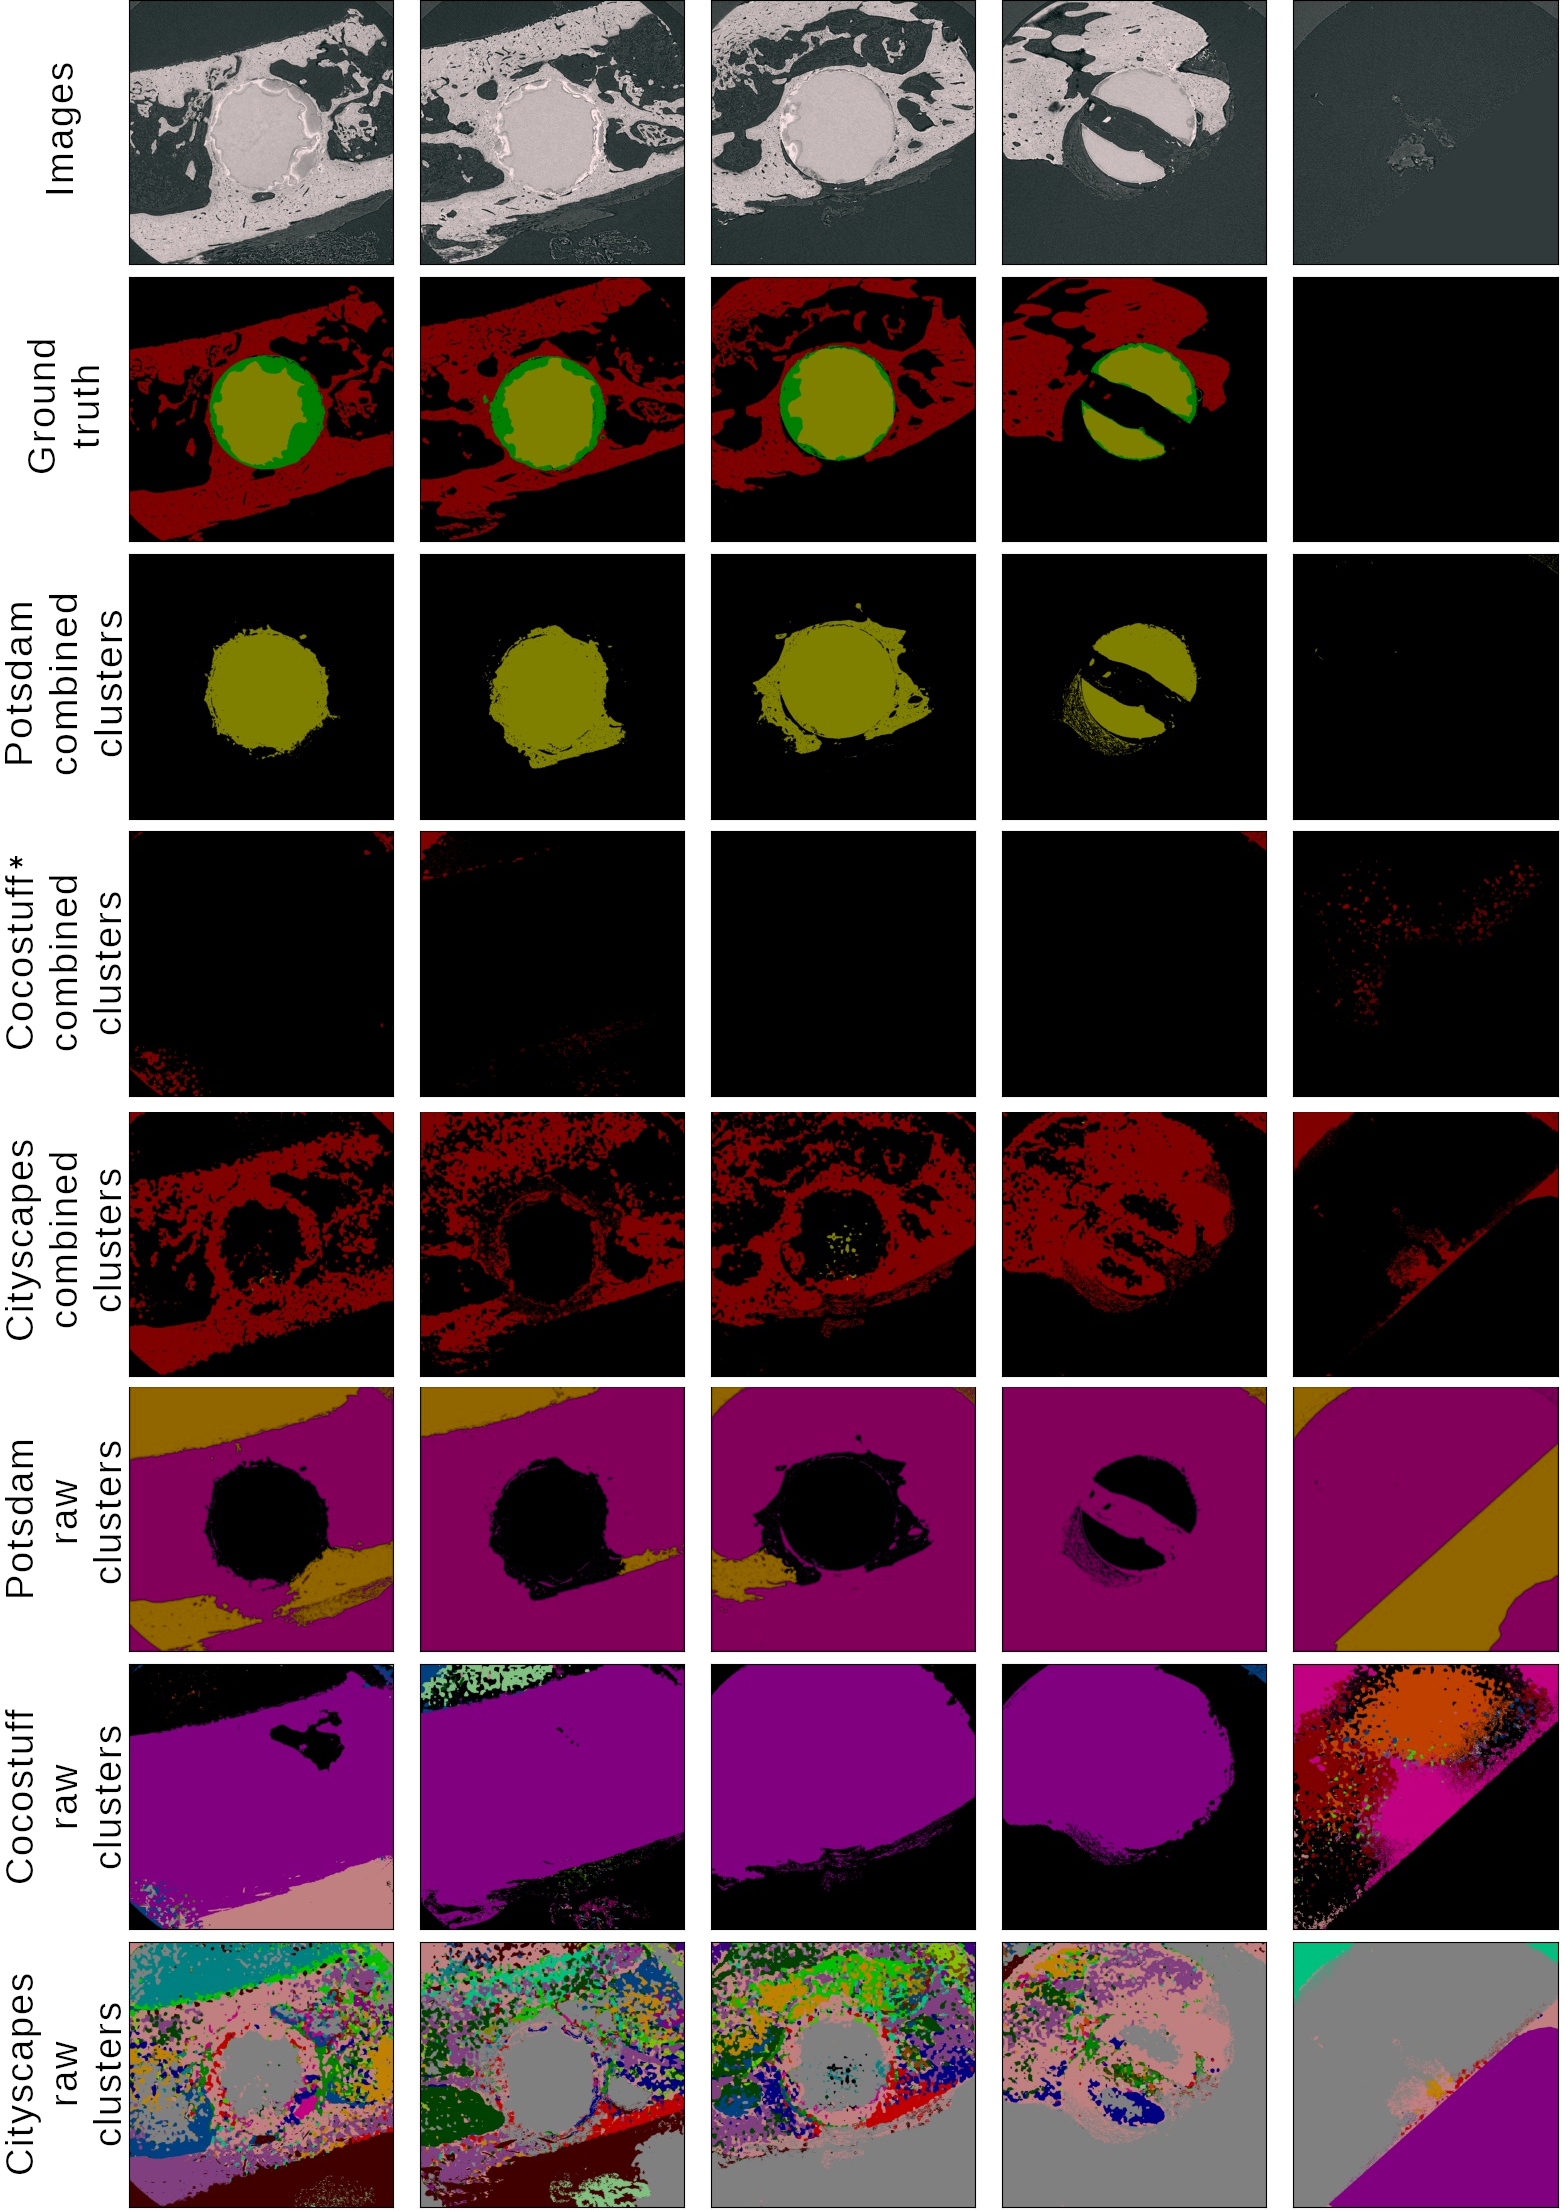
\includegraphics[width=\textwidth]{pictures/experiment_1/pretrained-models_cluster-predictions_example_predictions_2_small}\\
    \caption[Example Predictions from Provided Models]{Visualisation of image, ground truth, raw cluster predictions and clusters combined by their most likely match to ground truth label. Raw cluster colors correspond to cluster names in~\autoref{fig:correlation-matrix-pretrained}. Combined cluster assignment to ground truth labels is indicated by color. All shown slices belong to the second half of volume syn009HQ and are ordered according to spatial location in the volume. Every 100th slice is shown.
    \\ \textsuperscript{*}For more representative slices of combined clusters for COCO-Stuff see~\autoref{fig:more-cocostuff-predictions}.}
    \label{fig:pretrained-predictions}
\end{figure}

\begin{table}[!htb]
    \caption[IoU for Predictons with Pre-trained Models]{IoU of predicts done with pre-trained models. Predictions were made with different models, as identified by train data set (rows) for the same test set of the screws model. For each model, IoU of the ground truth label to the combination of clusters matching best according to correlation value is given (with manual corrections for COCO-Stuff), as well as the mean over all labels. A dash indicates that the label was not predicted. All values are rounded to the second decimal.}
    \label{tab:miou-pretrained-models}
    \makegapedcells      % in makecell
    \begin{tabular}{|>{\bfseries}l|c|c|c|c||c|}
        \hline
        Model & \textbf{\formatLabel{background}} & \textbf{\formatLabel{bone~~~}} & \makecell{\textbf{\formatLabel{degraded}}\\ \textbf{\formatLabel{screw}}} & \textbf{\formatLabel{screw}} & \textbf{mean} \\ \hline
        Potsdam & 0.71 & - & - & 0.36 & 0.27 \\ \hline
        Cocostuff & \makecell{0.69 \\(0.63)} & \makecell{0.35 \\(0.44)} & \makecell{0.00 \\(0.00)} & - & \makecell{0.26 \\(0.27)}\\ \hline
        Cityscapes & 0.65 & 0.37 &  - & 0.00 & 0.26\\ \hline
    \end{tabular}
\end{table}

%Potsdam
% model cluster to label assignment
% 0: buildings and clutter         -> screw
% 1: trees and vegetation          -> background
% 2: roads and cars                -> background
% cluster to label mapping
With the Potsdam model, the highest correlation was found between the Potsdam label \formatLabel{trees and vegetation} and \formatLabel{background} of the screws data set, though some \formatLabel{bone} pixels are also included (see~\autoref{fig:correlation-matrix-pretrained}).
Similarly, \formatLabel{roads and cars} correlated highly with \formatLabel{background} and to some degree also with \formatLabel{bone}.
The \formatLabel{buildings and clutter} cluster correlated to \formatLabel{screw} and and nearly to the same degree to \formatLabel{degraded screw} (in fact, all \formatLabel{screw} and \formatLabel{degraded screw} pixels were found in this cluster) and \formatLabel{bone}.
Additionally, \formatLabel{buildings and clutter} also contained \formatLabel{bone} and a few \formatLabel{background} pixels.
The other ground truth labels do not match as clearly, as seen in~\autoref{fig:correlation-matrix-pretrained}.

% combined clusters
When clusters were combined according to their most likely ground truth match (as seen in~\autoref{fig:correlation-matrix-pretrained}), Potsdam reached a slightly better overall \gls{miou} on the combined clusters and also the best \gls{iou} for a single label (\formatLabel{background} reached a \gls{miou} of 0.71), see ~\autoref{tab:miou-pretrained-models}.
% mIoU
\formatLabel{Bone} and \formatLabel{degraded screw} were not detected since no cluster correlated to them as clearly, and \formatLabel{screw} reached a \gls{iou} of 0.36.
When considering the predictions ~(\autoref{fig:pretrained-predictions}), the model mostly distinguishes two classes, one including \formatLabel{background} and \formatLabel{bone}, and one containing \formatLabel{screw} and \formatLabel{degraded screw}.
The differentiation between \formatLabel{screw/degraded screw} and \formatLabel{background/bone} was even visible in the fine cracks of the screw, as seen in~\autoref{fig:pretrained-predictions_syn009}.

\begin{figure}[!htb]
    \centering
    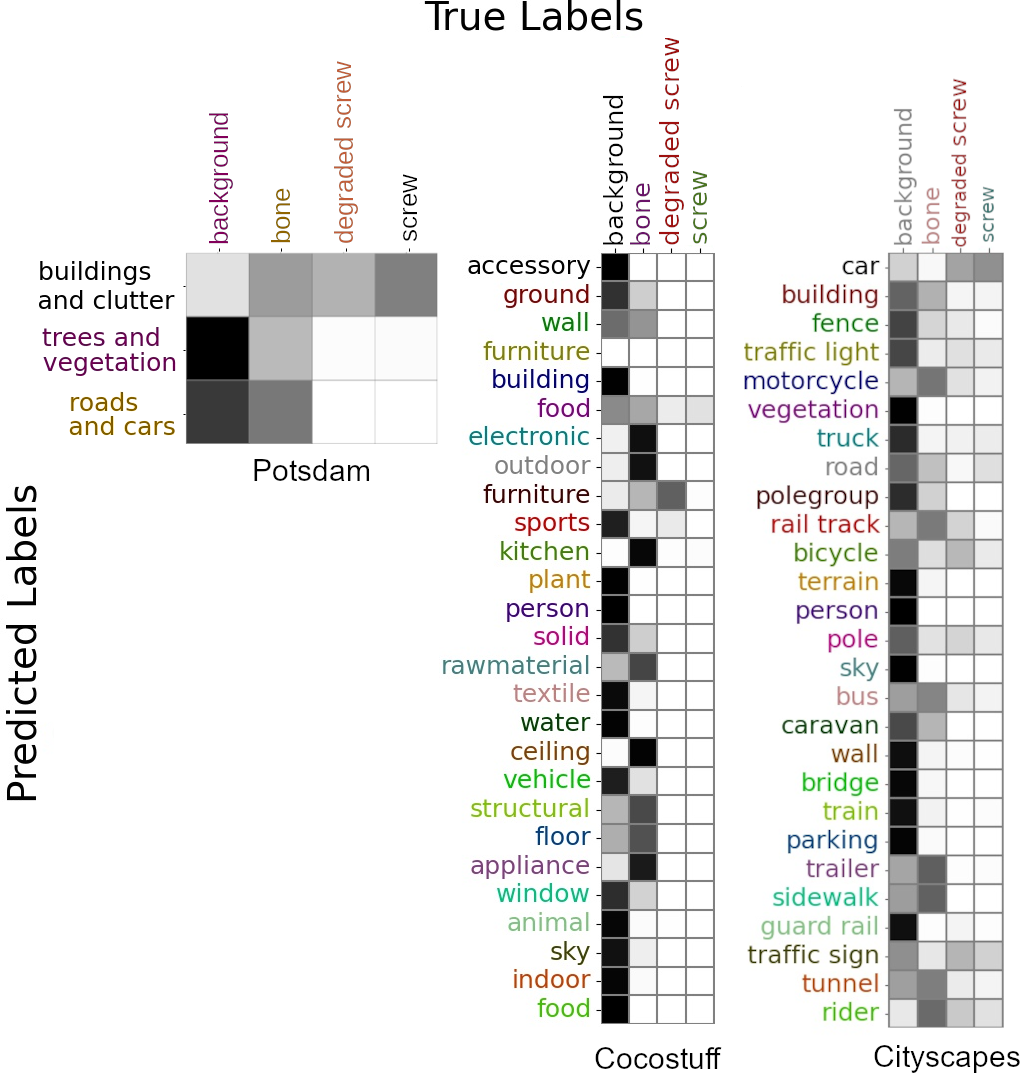
\includegraphics[width=\textwidth]{pictures/experiment_1/all_raw-cleaned_correlation_matrices}\\
    \caption[Correlation of Predicted Clusters to Labels]{Correlation matrix of ground truth labels and predicted clusters made with the three pre-trained models for the screws test set. Rows indicate predicted clusters, columns ground truth labels. \\ Ground truth label color indicates mapped model label. Dark color in the fields indicates a higher correlation coefficient than lighter color. Values are normed by row.}
    \label{fig:correlation-matrix-pretrained}
\end{figure}

\begin{figure}[!htb]
    \centering
    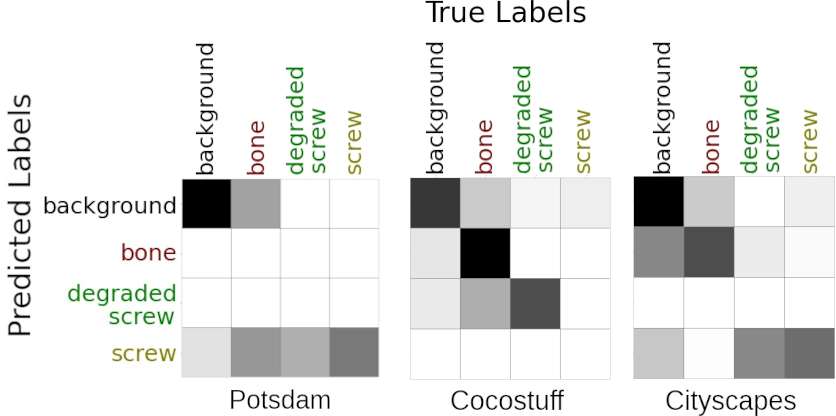
\includegraphics[width=0.9\textwidth]{pictures/experiment_1/all-combined_correlation_matrices}\\
    \caption[Correlation of Combined Clusters to Labels]{Correlation matrix of ground truth labels and merged predicted clusters made with the three pre-trained models for the screws test set. Rows indicate merged clusters, columns ground truth labels. Ground truth label color indicates mapped model label. Darker color in the fields indicates a higher correlation coefficient than lighter color. Values are normed by row. An exact model would be signified by a dark diagonal. Values are normed by row.}
    \label{fig:correlation-matrix-pretrained-combined}
\end{figure}

% Cocostuff
%model cluster - label assignment: 0: accessory, 1: ground, 2: wall, 3: furniture, 4: building, 5: food, 6: electronic, 7: outdoor, 8: furniture, 9: sports, 10: kitchen, 11: plant, 12: person, 13: solid, 14: rawmaterial, 15: textile, 16: water, 17: ceiling, 18: vehicle, 19: structural, 20: floor, 21: appliance, 22: window, 23: animal, 24: sky, 25: indoor, 26: food
% screws cluster to labels assignment: background = accessory, bone = food(1), degraded screw = sports, screw = kitchen
%cluster to label mapping
With the COCO-Stuff model, mapping single clusters to the ground truth labels via Hungarian matching found the following label assignments: the \formatLabel{accessory} cluster mapped to \formatLabel{background}, \formatLabel{food} (first occurrence) to \formatLabel{bone}, \formatLabel{sports} to \formatLabel{degraded screw} and \formatLabel{kitchen} to \formatLabel{screw}.
However, as seen in the correlation matrix (\autoref{fig:correlation-matrix-pretrained}), often multiple other categories were fully (or mostly) encompassed in one of the ground truth labels.
For example, the ground truth label \formatLabel{background} included most pixels belonging to \formatLabel{accessory, ground, wall, building, sport, plant, person, solid, textile, water, vehicle, window, animal, sky, indoor}, and the second \formatLabel{food} cluster;
the \formatLabel{bone} label included large parts of \formatLabel{vehicle, electronic, outdoor, kitchen, raw material, ceiling, structural, floor} and \formatLabel{appliance}.
The ground truth label \formatLabel{degraded screw} contained most \formatLabel{furniture} pixels, but did not correlate much with \formatLabel{sports}, to which it was mapped with Hungarian matching.
The correlation of \formatLabel{screw} was very weak for all clusters.
%combined clusters
When clusters were combined according to their most likely ground truth match (according to correlation value), three labels were reproduced: \formatLabel{background} (\gls{iou} of 0.69), \formatLabel{bone} (\gls{iou} of 0.37), and \formatLabel{degraded screw} (\gls{iou} 0.00).
However, mostly background was predicted, as seen in~\autoref{fig:pretrained-predictions}.
\begin{figure}[!htb]
    \centering
    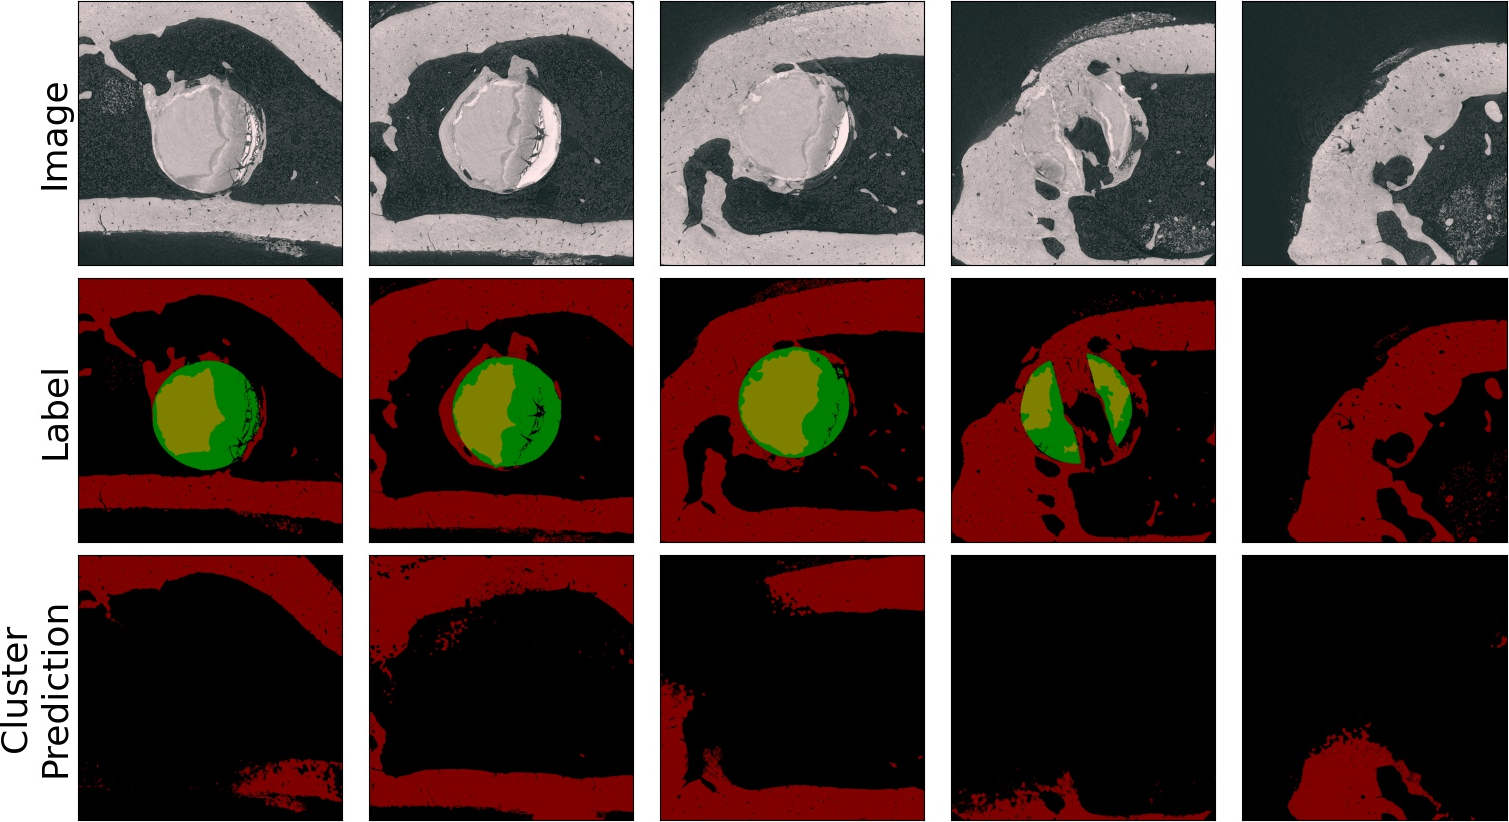
\includegraphics[width=0.95\textwidth]{pictures/experiment_1/cocostuff-combined_example_predictions_0_small}\\
    \caption[Additional Combined Clusters of COCO-Stuff]{Visualisation of image, ground truth, and clusters combined by their most likely match to ground truth labels for COCO-Stuff predictions. All shown slices belong to the second half of volume 113729HQMg5 and are ordered according to spatial location in the volume. Every 100th slice is shown.}
    \label{fig:more-cocostuff-predictions}
\end{figure}

% manual clusters
When looking at the predictions in~\autoref{fig:pretrained-predictions}, the big purple \formatLabel{food} cluster stands out, since it seems to neatly encompass the full bone (including bone marrow and screw) on some slices (on other predictions it encompasses only bone marrow), see~\autoref{fig:more-cocostuff-predictions}.
It was decided to manually assign this cluster to \formatLabel{bone}, since it mostly included bone and also bone marrow. 
The high correlation value with \formatLabel{background} was calculated because in the ground truth, bone marrow was mostly assigned to \formatLabel{background} and not \formatLabel{bone}, since segmentation was based on a thresholding method.
With this manual assignment, predictions of \formatLabel{bone} improved slightly (from \gls{miou} of 0.35 to 0.44), while \gls{iou} of \formatLabel{background} slightly decreased from 0.69 to 0.63.
The \formatLabel{degraded screw} label did not change at all, as was to be expected, since no pixel was removed or added to this label.
A visualisation of this manual assignment in comparison to assignment by correlation value can be found in~\autoref{fig:cocostuff-compare-manualcombine-predictions}.
\begin{figure}[!htb]
    \centering
    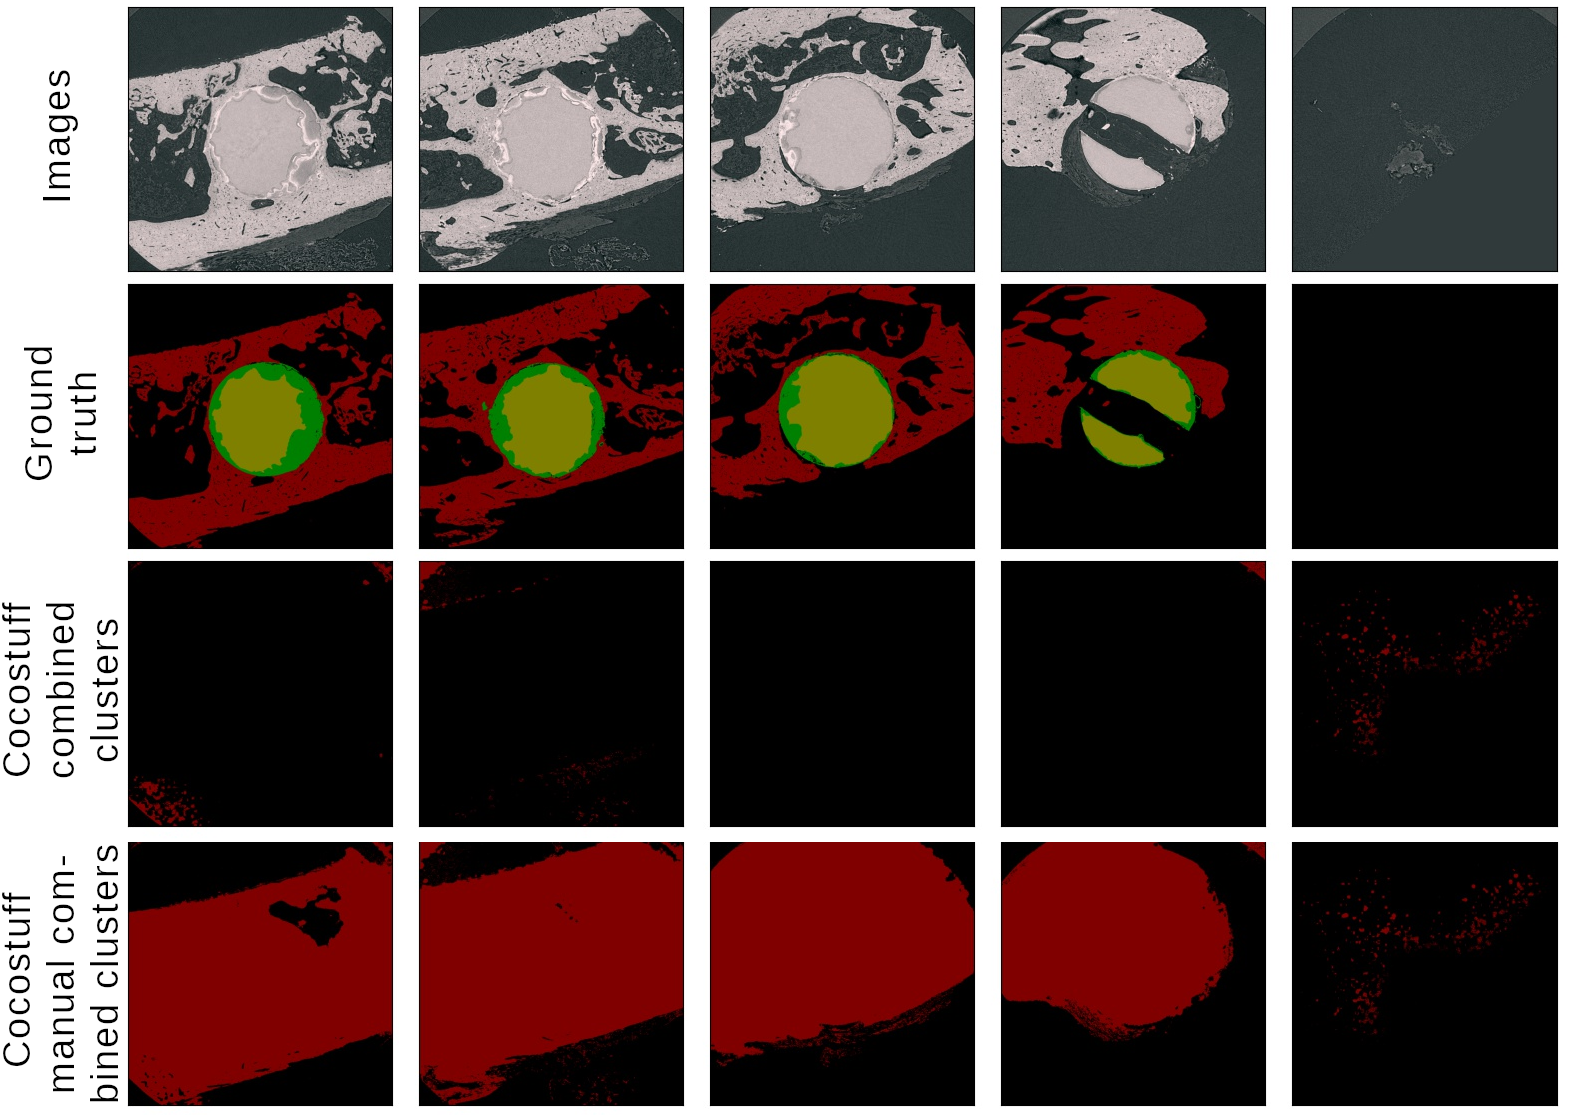
\includegraphics[width=\textwidth]{pictures/experiment_1/cocostuff-compare-manual-combined_example_predictions_2}\\
    \caption[Manually Combined Clusters of COCO-Stuff]{Image, ground truth, and manually combined clusters of predictions made with the COCO-Stuff model. All shown slices belong to the second half of volume syn009HQ (which was neither part of train nor validation set) and are ordered according to spatial location in the volume. Every 100th slice is shown.}
    \label{fig:cocostuff-compare-manualcombine-predictions}
\end{figure}

% Cityscapes
%model cluster to label assignment:  0: car, 1: building, 2: fence, 3: traffic light, 4: motorcycle, 5: vegetation, 6: truck, 7: road, 8: polegroup, 9: rail track, 10: bicycle, 11: terrain, 12: person, 13: pole, 14: sky, 15: bus, 16: caravan, 17: wall, 18: bridge, 19: train, 20: parking, 21: trailer, 22: sidewalk, 23: guard rail, 24: traffic sign, 25: tunnel, 26: rider
% road = background, bus = bone, rail track = degraded screw, truck = screw
%cluster to label mapping
With the Cityscapes model, mapping single clusters to the ground truth labels with Hungarian matching yields the following assignments: \formatLabel{road} mapped to \formatLabel{background}, \formatLabel{bus} to \formatLabel{bone}, \formatLabel{rail track} to \formatLabel{degraded screw} and \formatLabel{truck} to \formatLabel{screw}.
Again, these mappings were not the only candidates as seen in~\autoref{fig:correlation-matrix-pretrained-combined}.
Large parts of \formatLabel{building, fence, traffic light, vegetation, truck, polegroup, terrain, person, pole, sky, caravan, wall bridge, train, parking}, and \formatLabel{guard rail} also correlated with \formatLabel{background}, while large parts of \formatLabel{motorcycle, rail track, bus, trailer, sidewalk, tunnel}, and \formatLabel{rider} also correlated strongly with \formatLabel{bone}.
On the other hand, the correlation of \formatLabel{rail track} to the \formatLabel{degraded screw} label (which it was assigned to with Hungarian matching) was also very weak, while the correlation of \formatLabel{furniture} is higher.
% combined clusters
Combining all clusters by their most likely ground truth mapping produced good predictions of \formatLabel{background} (\gls{iou} of 0.63), intermediate predictions of \formatLabel{bone} (\gls{iou} 0.37), and basically no predictions of \formatLabel{degraded screw} and \formatLabel{screw}.
This was also reflected in the correlation matrix (\autoref{fig:correlation-matrix-pretrained-combined}), where only \formatLabel{background} and \formatLabel{bone} correlated at a higher rate.

\begin{figure}[!htb]
    \centering
    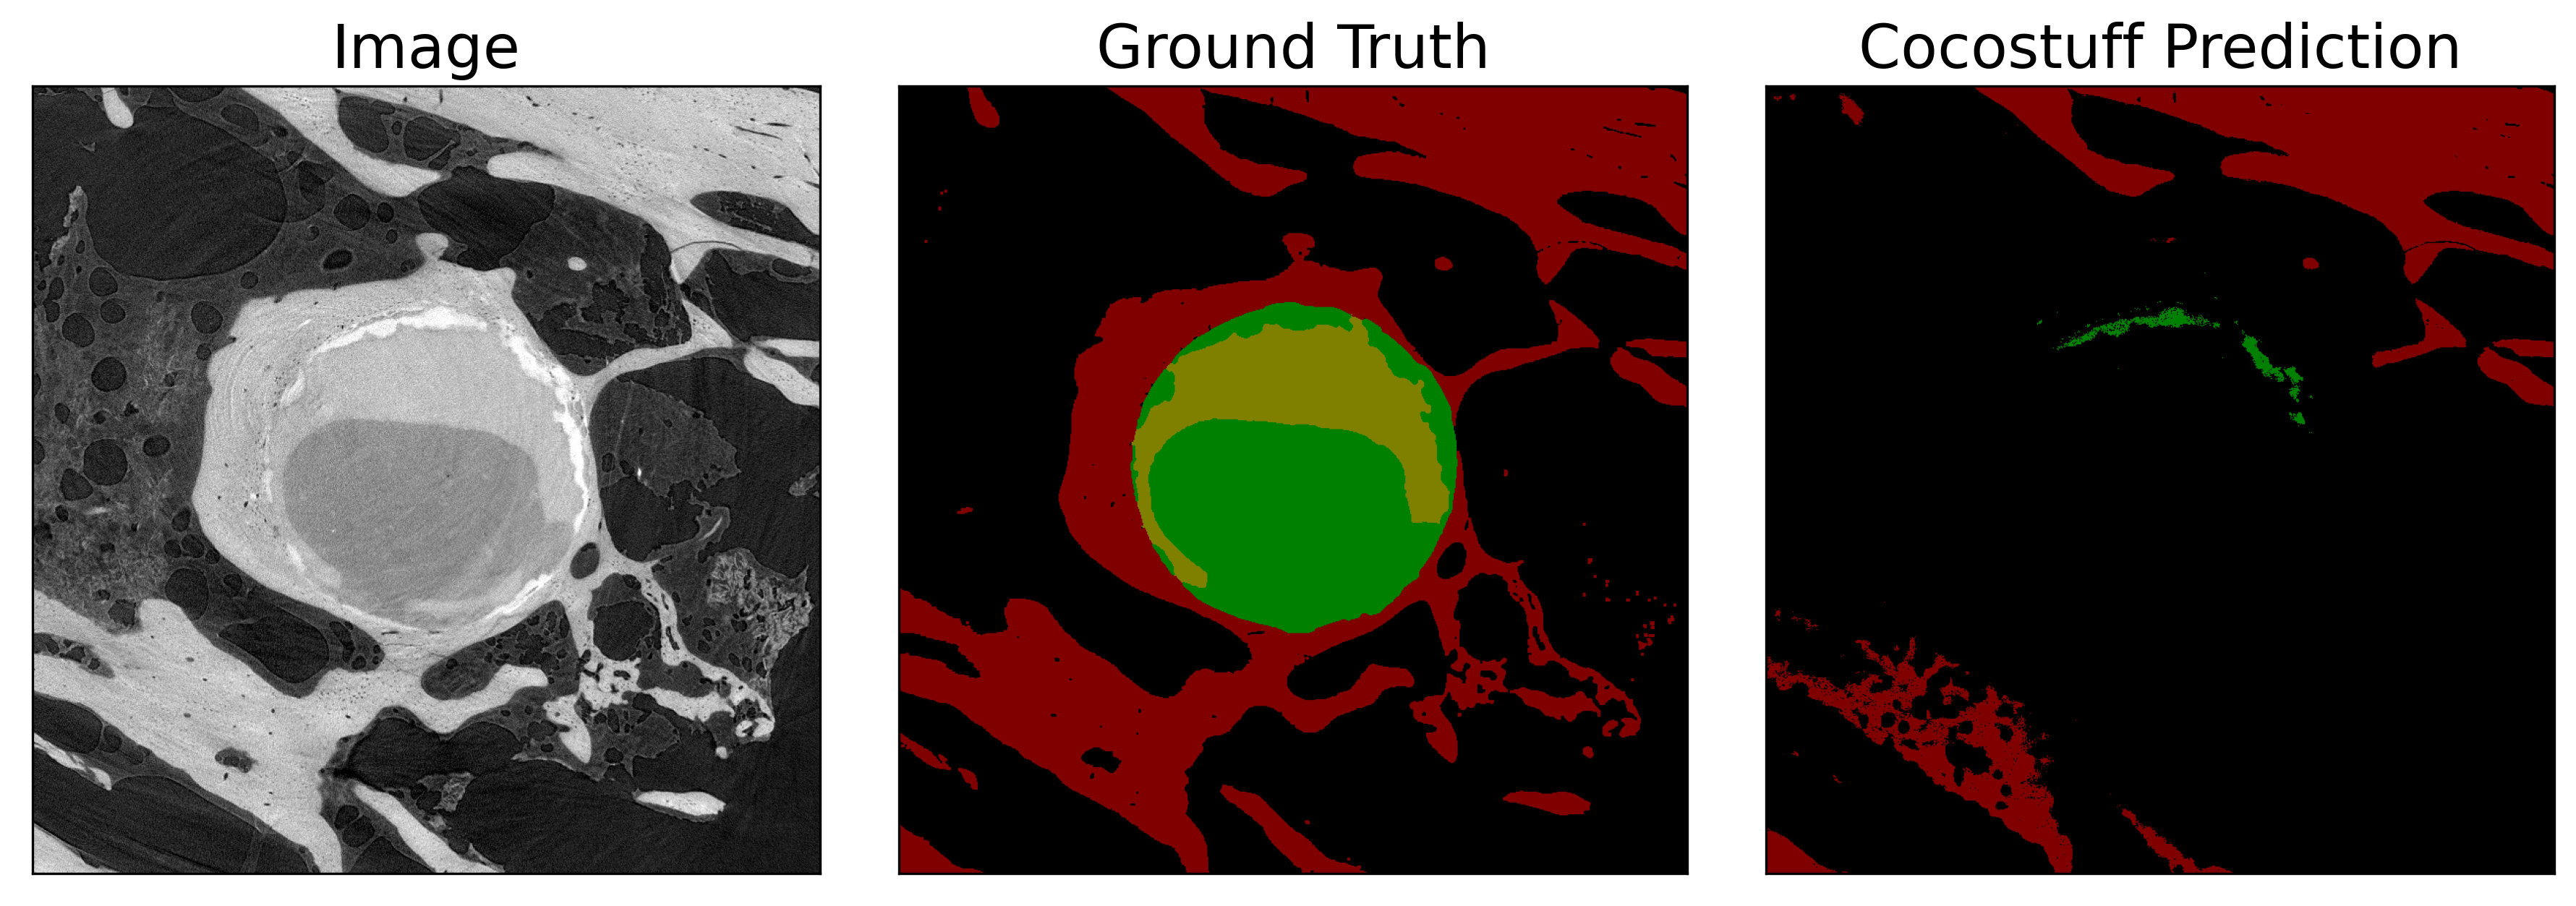
\includegraphics[width=\textwidth]{pictures/experiment_1/113734HQMg5_direction0_slice0670_cocostuff_prediction_with_degraded_screw_prediction}\\
    \caption[Degraded Screw Prediction of COCO-Stuff]{Image, ground truth and prediction with the COCO-Stuff model of slice 670 from volume 113734HQMg5, to show size and location of \formatLabel{degraded screw} predictions. This slice has the biggest area of the \formatLabel{degraded screw} prediction (2328 pixels), which is located at the edge of the ground truth label. Most other slices only contain very few pixels.}
    \label{fig:cocostuff-degradedscrew-example}
\end{figure}

Generally, there were only a few pixels identified as \formatLabel{screw}.
Only 267 (often not concurrent slices) of the 3000~slices test set contained \formatLabel{screw} pixels.
Additionally, these patches were very small, and only comprise few pixels each, which were aligned around the edges of the ground truth label, as seen in~\autoref{fig:cocostuff-degradedscrew-example}.
Thus overall-correlation of the few pixels, that were found, was quite high, as seen in \autoref{fig:correlation-matrix-pretrained-combined}, meaning there were few false positives.
However, most real \formatLabel{screw} pixels are identified (wrongly) as \formatLabel{background}.
Overall, the \gls{miou} of the combined clusters for the Cityscapes model was~0.26.
% contain the floats in section
\afterpage{\FloatBarrier}

% wrap up for all three
None of the three models was able to differentiate all ground truth labels.
At least one label was missing in each.
Additionally, the predictions were often not very good.
All three models reached \gls{iou} values between 0.6 and 0.7 for \formatLabel{background}, around 0.3 for \formatLabel{bone} (if it was predicted at all) and 0.36 (Potsdam) or nearly 0 (Cityscapes) for \formatLabel{screw}.
\formatLabel{Degraded screw} was only predicted with COCO-Stuff, but the \gls{iou} was nearly 0 there, too.


\subsubsection{Experiment 2: Train on Scientific Data Set}\label{subsubsec:results-experiment2res}

% runtimes and batch sizes
Training was done on different configurations with different image resolutions and thus, batch sizes.
Batch size of the base case was 8, for the 200~px random cropped regime it could be increased to 16, and for the 96~px random cropped regime it could be doubled to 32 again.
This means, runtimes varied between 1.5~hours and more than a day, depending on the configuration.
An overview on the runtimes can be found in ~\autoref{tab:runtimes}.
Because the batch size varied, the number of steps in one epoch\footnote{One epoch is a full run through all training examples, and steps are defined as one run through a batch. For multi-GPU-training a step is one run through a batch on all GPUs.} also varied, but due to different image sizes, the number of seen pixels are the same between steps.
For example, due to the four times higher batch size (and 5.2~times smaller image size), the model trained on the 96~px random cropped data set was trained on four times more training images per step, but only 0.8~times the number of pixels in comparison to the base case.
Similar proportions are true for the 200~px random cropped model, where the batch size was half the size in comparison to the base case, and the image size was 0.4~times smaller.\footnote{That means, the two random cropped regimes were trained on nearly the same pixel numbers at each step.}

\begin{table}[!bht]
    \caption[Best Models Accuracy per Fold]{Best models accuracy (proportion of correctly classified pixels) per fold. Models are identified by cropping regime, resolution, and fold.\textsuperscript{*} For each model the accuracy on the validation set and [step] at which it occurred is given. Additionally, mean and standard deviation of accuracy over folds is reported. Values are rounded to the second decimal. Note, that step numbers between models do not correspond, and folds between leave-one-out (LOO) and all others differ.}
    \label{tab:accuracy-step-by-fold}
    \makegapedcells      % in makecell
    \centering
    \begin{tabular}{|>{\bfseries}c|>{\raggedright\arraybackslash}p{0.11\textwidth}|>{\raggedright\arraybackslash}p{0.11\textwidth}|>{\raggedright\arraybackslash}p{0.115\textwidth}|>{\raggedright\arraybackslash}p{0.11\textwidth}|>{\raggedright\arraybackslash}p{0.11\textwidth}||r|}
        \hline
        \makecell[cb]{} & \makecell[c]{\textbf{Fold 0}} & \makecell[c]{\textbf{Fold 1}} &
        \makecell[c]{\textbf{Fold 2}} & \makecell[c]{\textbf{{Fold 3}}} & \makecell[c]{\textbf{Fold 4}} & \textbf{mean}\\ \hline
        % base-case
        \makecell[c]{\hspace{1mm}base\\case} & \makecell[r]{0.71 \\\emph{\small[1,249]}} & \makecell[r]{0.71 \\\emph{\small[2,718]}} & \makecell[r]{0.65 \\\emph{\small[499]}} & \makecell[r]{0.70 \\\emph{\small[499]}} & \makecell[r]{0.73 \\ \emph{\small[3,124]}} & \makecell[r]{0.70\\ ± 0.03} \\ \hline
        % random 200px  
        \makecell{random\\cropped\\200~px} & \makecell[r]{0.63 \\\emph{\small [1,359]}}	&	\makecell[r]{0.64 \\\emph{\small [1,359]}} & \makecell[r]{ 0.66 \\ \emph{\small [1,359]}} & \makecell[r]{ 0.67 \\\hspace{-2.2mm}\emph{\small [11,679]}} & \makecell[r]{ 0.58 \\ \emph{\small [249]}} & \makecell[r]{0.64\\ ± 0.04}\\ \hline
        % radom 96px  
        \makecell{random\\cropped\\96~px} & \makecell[r]{0.76 \\ \emph{\small [1,539]}} & \makecell[r]{0.61 \\ \emph{\small [8,419]}} & \makecell[r]{ 0.57 \\ \emph{\small [249]}} & \makecell[r]{0.63 \\\emph{\small [4,549]}} & \makecell[r]{0.59 \\ \emph{\small [249]}} & \makecell[r]{0.63\\± 0.08} \\ \hline
        % LOO
        & \makecell[c]{\textbf{LOO 0}} & \makecell[c]{\textbf{LOO 1}} &
        \makecell[c]{\textbf{LOO 2}} & \makecell[c]{\textbf{{LOO 3}}} & \makecell[c]{\textbf{LOO 4}} & \textbf{mean}\\ \hline
        \makecell{leave-\\one-\\out} & \makecell[r]{0.69 \\ \emph{\small [6,845]}} & \makecell[r]{0.66 \\ \emph{\small [7,595]}} & \makecell[r]{ 0.83 \\ \emph{\small [29,447]}} & \makecell[r]{0.68 \\\emph{\small [1,999]}} & \makecell[r]{0.68 \\ \emph{\small [8,877]}} & \makecell[r]{0.71\\± 0.07} \\ \hline
    \end{tabular}
    \raggedright
    \\ \small\textsuperscript{*}Extra cluster regimes are not reported here, since accuracy is misleading in these.
\end{table}

\begin{table}[p]
    \caption[Best Models mIoU per Fold]{Best models mIoU per fold. Models are identified by cropping regime, resolution, and fold.\textsuperscript{*} For each model the mIoU on the validation set and standard deviation is given. Additionally, mean and standard deviation of mIoU over folds is reported. Values are rounded to the second decimal. Note, that folds between leave-one-out (LOO) cross-validation and all others differ.}
    \label{tab:miou-by-fold}
    \makegapedcells      % in makecell
    \centering
    \begin{tabular}{|>{\bfseries}c|>{\raggedright\arraybackslash}p{0.11\textwidth}|>{\raggedright\arraybackslash}p{0.11\textwidth}|>{\raggedright\arraybackslash}p{0.115\textwidth}|>{\raggedright\arraybackslash}p{0.11\textwidth}|>{\raggedright\arraybackslash}p{0.11\textwidth}||r|}
        \hline
        \makecell[cb]{} & \makecell[c]{\textbf{Fold 0}} & \makecell[c]{\textbf{Fold 1}} &
        \makecell[c]{\textbf{Fold 2}} & \makecell[c]{\textbf{{Fold 3}}} & \makecell[c]{\textbf{Fold 4}} & \textbf{mean}\\ \hline
        % base-case
        \makecell[c]{\hspace{1mm}base\\case} & \makecell[r]{0.49 \\ ± 0.35} & \makecell[r]{0.49 \\ ± 0.34} & \makecell[r]{0.43 \\± 0.29} & \makecell[r]{0.45 \\±0.30} & \makecell[r]{0.50 \\ ± 0.34} & \makecell[r]{0.47\\ ± 0.03} \\ \hline
        % random 200px  
        \makecell{random\\cropped\\200~px} & \makecell[r]{0.44 \\± 0.33}	&	\makecell[r]{0.48 \\± 0.35} & \makecell[r]{ 0.44 \\ ± 0.30} & \makecell[r]{ 0.44 \\± 0.32} & \makecell[r]{ 0.39 \\ 27} & \makecell[r]{0.44\\ ± 0.03}\\ \hline
        % radom 96px  
        \makecell{random\\cropped\\96~px} & \makecell[r]{0.57 \\ ± 0.30} & \makecell[r]{0.39 \\ ± 0.28} & \makecell[r]{ 0.38 \\ ± 0.20} & \makecell[r]{0.46 \\± 0.33} & \makecell[r]{0.41 \\ ± 0.21} & \makecell[r]{0.44\\± 0.08} \\ \hline
        & \makecell[c]{\textbf{LOO 0}} & \makecell[c]{\textbf{LOO 1}} &
        \makecell[c]{\textbf{LOO 2}} & \makecell[c]{\textbf{{LOO 3}}} & \makecell[c]{\textbf{LOO 4}} & \textbf{mean}\\ \hline
        \makecell{leave-\\one-\\out} & \makecell[r]{0.54 \\ ± 0.33} & \makecell[r]{0.41 \\ ± 0.29} & \makecell[r]{ 0.61 \\ ± 0.39} & \makecell[r]{0.47 \\± 0.32} & \makecell[r]{0.47 \\ ± 0.34} & \makecell[r]{0.50\\± 0.08} \\ \hline
    \end{tabular}
%Extra cluster regimes are not reported here, since \gls{miou} is misleading in these. 
    \caption[Best Models IoU per Label]{Best models IoU per label. Models are identified by cropping regime and resolution or cross-validation scheme.\textsuperscript{*} For each model, IoU and standard deviation of IoU for each label (as well as mean over all labels and standard deviation between labels) on the validation set over the cross-validation is given. Values are rounded to the second decimal.}
    \label{tab:miou-by-label}
    \makegapedcells      % in makecell
    \centering
    \begin{tabular}{|>{\bfseries}c|>{\raggedright\arraybackslash}p{0.13\textwidth}|>{\raggedright\arraybackslash}p{0.13\textwidth}|>{\raggedright\arraybackslash}p{0.15\textwidth}|>{\raggedright\arraybackslash}p{0.13\textwidth}||>{\raggedright\arraybackslash}p{0.1\textwidth}|}
        \hline
        & \makecell[c]{\textbf{\formatLabel{back-}} \\ \textbf{\formatLabel{ground}}} & \makecell[c]{\textbf{\formatLabel{bone}}} &
        % else we get an ugly linebreak in cell
        \makecell[c]{\hspace{-0.5mm}\textbf{\formatLabel{degraded}} \\ \textbf{\formatLabel{screw}}} & \makecell[c]{\textbf{\formatLabel{screw}}} & \makecell[c]{\textbf{mean}} \\ \hline
        %base-case
        \makecell{base case} & \makecell[r]{0.59 \\± 0.04} & \makecell[r]{0.69 \\± 0.11} & \makecell[r]{0.00 \\± 0.00} & \makecell[r]{0.61 \\± 0.03} & \makecell[r]{0.47\\± 0.32}  \\ \hline
        % random 200px  
        \makecell{random\\cropped\\200~px} & \makecell[r]{0.48 \\± 0.04}	&	\makecell[r]{0.62 \\± 0.11} & \makecell[r]{0.00 \\± 0.00} & \makecell[r]{0.66 \\± 0.09} & \makecell[r]{0.44\\± 0.30}	 \\ \hline
        % radom 96px  
        \makecell{random\\cropped\\96~px} & \makecell[r]{0.52 \\± 0.10} & \makecell[r]{0.61 \\± 0.10} & \makecell[r]{0.06 \\± 0.05} & \makecell[r]{0.57 \\± 0.13} & \makecell[r]{0.44\\± 0.26} \\ \hline
        % LOO
        \makecell{leave-one-\\out} & \makecell[r]{0.61 \\± 0.12}	&	\makecell[r]{0.74 \\± 0.08} & \makecell[r]{0.02 \\± 0.03} & \makecell[r]{0.62 \\± 0.13} & \makecell[r]{0.50\\± 0.32}	 \\ \hline
    \end{tabular}
    \raggedright
    \\ \small\textsuperscript{*}Extra cluster regimes are not reported here, since \gls{iou} is misleading in these.
\end{table}

%weights
Since cropping changes the images used for training, the parameter tuning needed to be done separately for each training.
Only the base case and the extra cluster trainings could be run with the same parameters, since there were no differences between the training data (only differences in configurations to allow for extra clusters).
An overview of the parameters can be found in the appendix in ~\autoref{tab:training-parameters}.

% base case
The base case was trained on the five-cropped data set, as explained before.
% explain images
Example predictions of the different base case folds can be found in~\autoref{fig:example-predictions-folds-base-case}.
Predictions between folds differed slightly, especially in slices stemming from the edges of the volumes (see last image in~\autoref{fig:example-predictions-folds-base-case}).
Additionally, predictions of areas outside the sample were often assigned to different labels, as seen in the second to fourth images in~\autoref{fig:example-predictions-folds-base-case}.
%explain mIoU
As seen in \autoref{tab:miou-by-fold}, \gls{miou} varied between folds and peaked around 0.50 in the different folds.
The course of the accuracy is basically the same, but shifted upwards, as seen in~\autoref{fig:accuracy-per-fold}, thus in the following, the focus is laid on the \gls{miou}.
In all five folds, this peak (the best model) was reached relatively early during training, between the~500th and~3,200th step~(\autoref{tab:accuracy-step-by-fold}).
Afterwards, \gls{miou} decreased to around~0.35 to~0.40.
As seen in \autoref{fig:miou-per-fold-label} and \autoref{tab:miou-by-label}, performance between the labels highly differed.
Label \formatLabel{bone} performed best (\gls{iou} in the folds was 0.69~±~0.11), followed by \formatLabel{screw} (\gls{iou} of 0.61~±~0.03) and \formatLabel{background} (\gls{iou} of 0.59~±~0.04), while \formatLabel{degraded screw} could not be detected at all (\gls{iou} of 0.00~±~0.00).
This difference in performance can also be seen in the accuracy values of the folds (see~\autoref{tab:accuracy-step-by-fold}), which are generally higher than the \gls{miou}, but similarly distributed, as seen in~\autoref{fig:accuracy-mIoU-boxplots}.
\afterpage{\FloatBarrier}
% comparison to random cropped
Trainings on the random cropped data sets did not differ much from the five-cropped base case in regard to \gls{miou} (which was 0.44~for both resolutions used), but there were differences in \gls{iou} between folds and labels (as seen in~\autoref{tab:miou-by-label},~\autoref{fig:miou-per-fold},~and ~\autoref{fig:miou-per-fold-label}).
Additionally, it can be seen in~\autoref{fig:example-predictions-fold2} that differences in predictions between the cropping regimes occurred on similar occasions (on slices at the edge of the 3D volumes, and outside the specimen) as differences between folds.
Divergence of \gls{miou} between folds was very pronounced in the 96~px random cropped regime, where fold~0 performed a lot better than all other folds (nearly two standard deviations difference in \gls{miou}).
For the training made on the 200~px random cropped data set, the best models were, again, reached early during training, between step 249 and 1,359.\footnote{Since image size and batch sizes differed between base case and random cropped trainings, this step number does not correspond to the base case in terms of training examples or pixels seen.
The 200~px random cropped regime saw two times more, the 96~px random cropped regime four times more training examples per step, but they both saw only 0.8 times the pixel number of the base case.}


\begin{figure}[p]
    \centering  %trim={<left> <lower> <right> <upper>}
    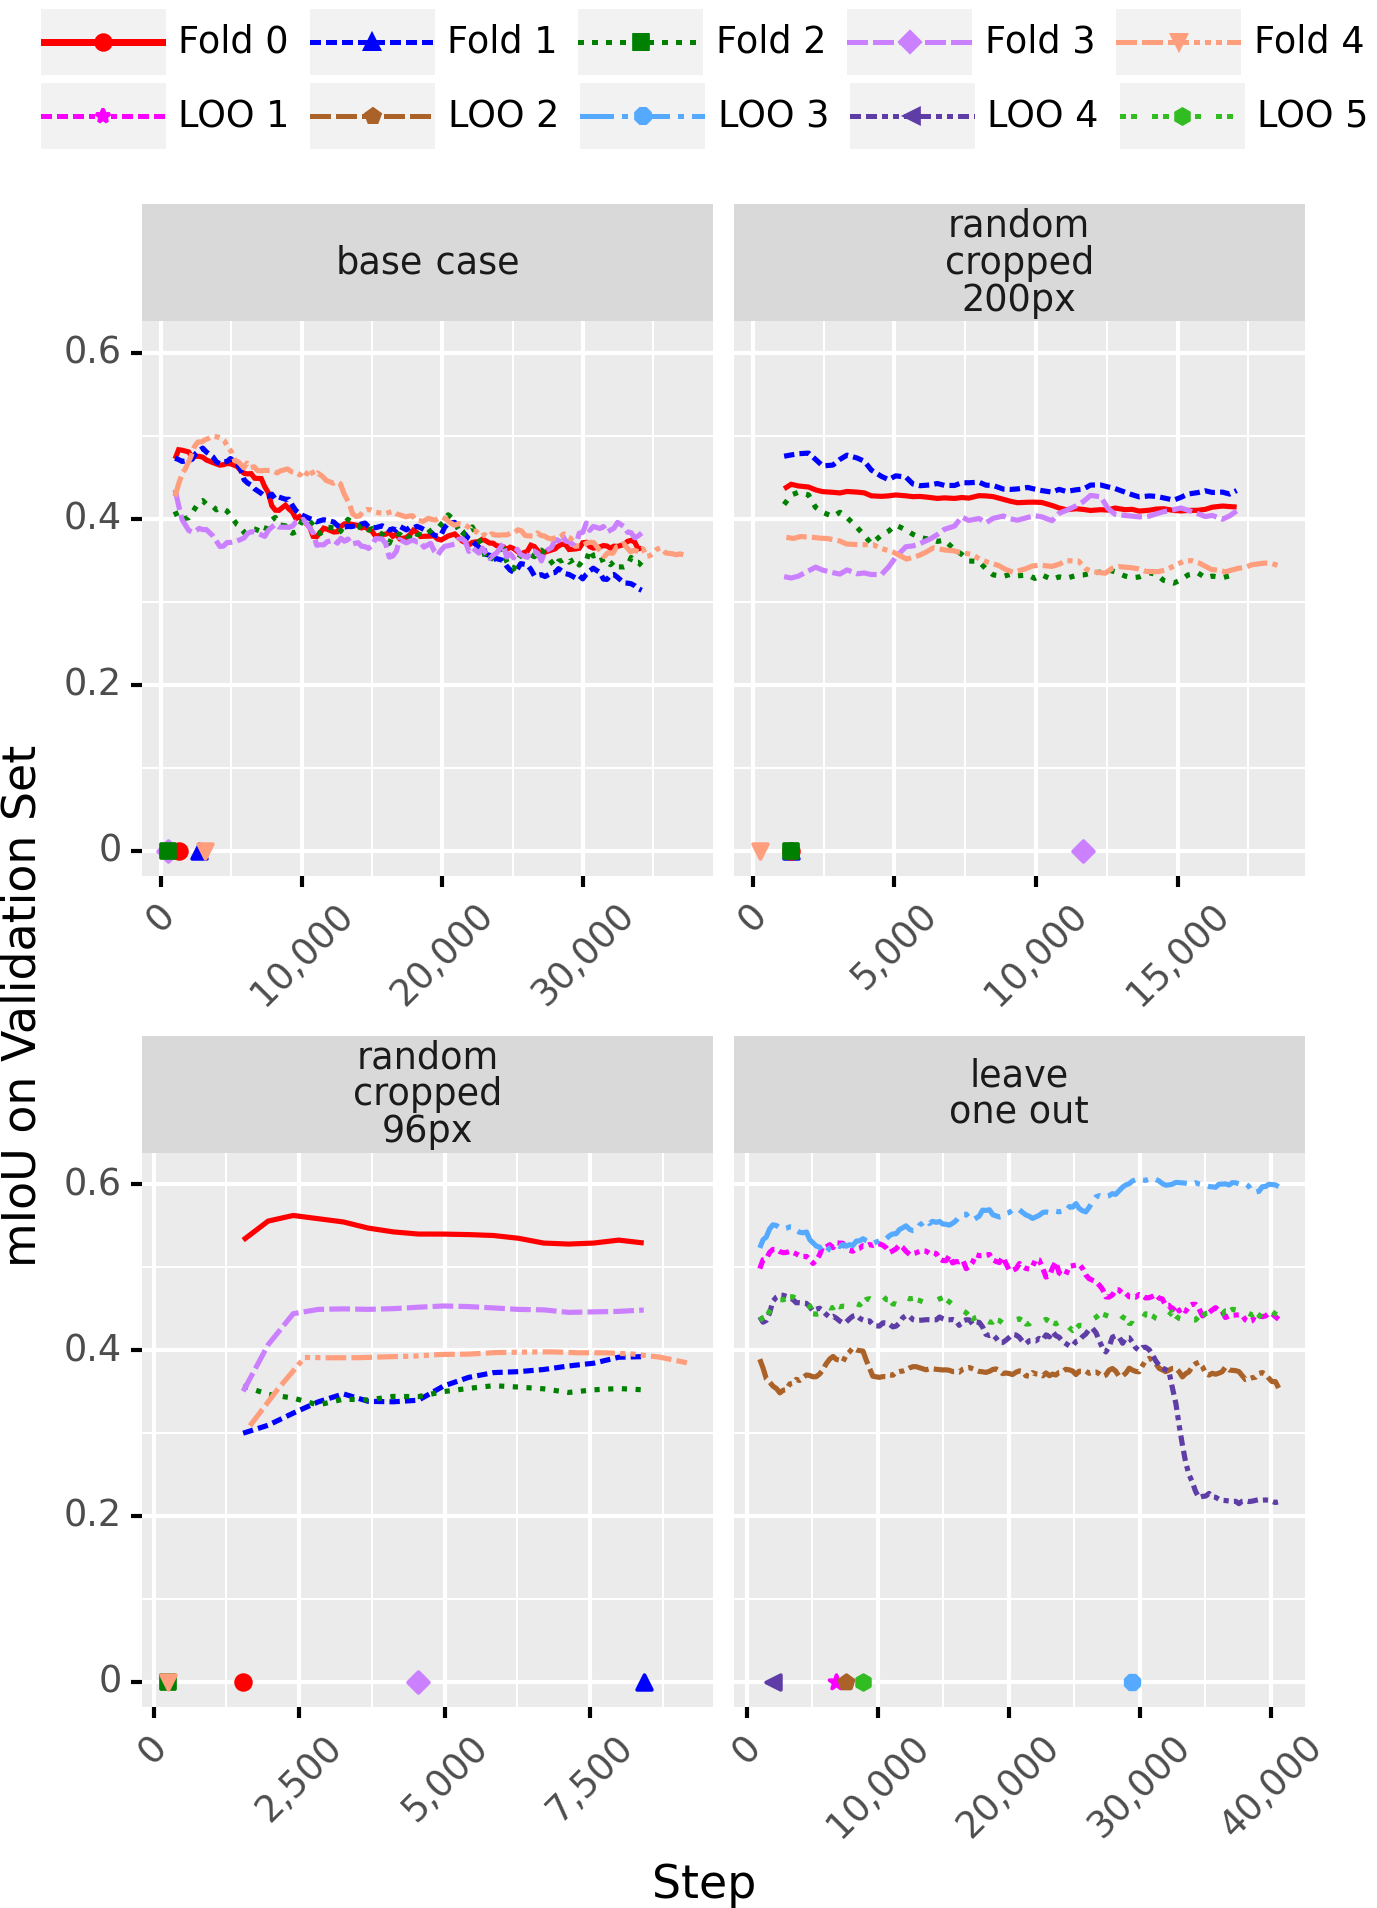
\includegraphics[width=\textwidth]{pictures/experiment_2/mIoU_base-case_final_base-case_loo_random_cropped_final_random_cropped_res96_final}\\
    \caption[Fold-wise Development of mIoU]{Fold-wise development of mIoU. For each cross-validation, the moving average (over three data points) of the mIoU per fold is displayed. So the first three data points are not depicted in the plots. Additionally, on the x-axis the step number of the best overall model per fold (in terms of mIoU) is marked.\\}  % to have only this figure on page
    \label{fig:miou-per-fold}
\end{figure}

\begin{figure}[p]
    \centering
    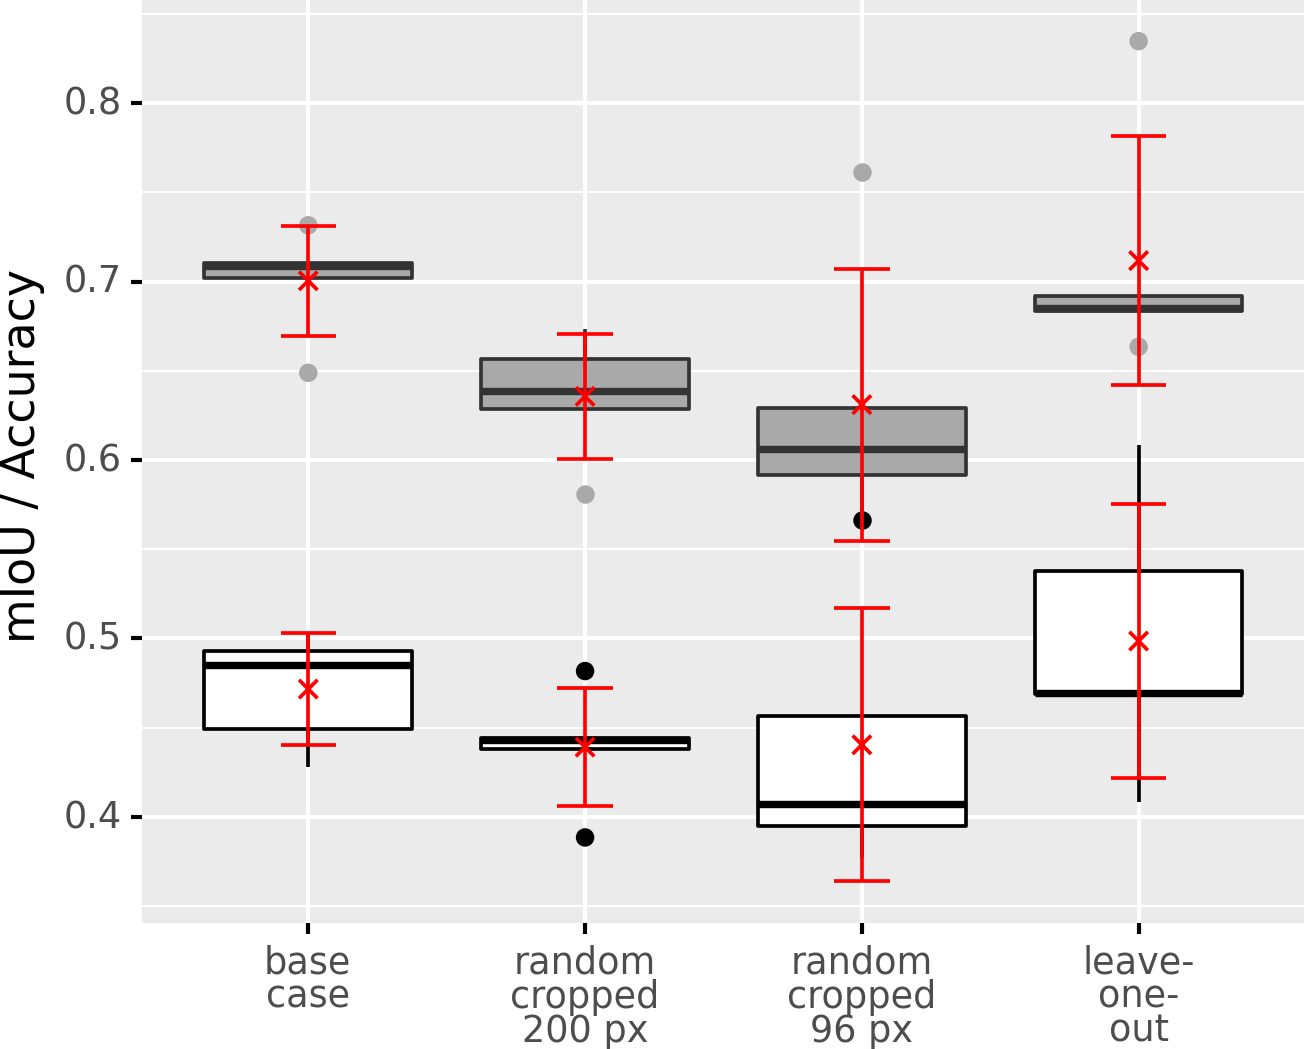
\includegraphics[width=0.8\textwidth]{pictures/experiment_2/compare_all_model_stats_mIoU_accuracy}\\
    \caption[Boxplots of mIoU and Accuracy for Best Models]{Boxplots of the accuracy (grey) and mIoU (white) for all folds of a configuration. Boxplots indicate the median as solid line, the hinges indicate the inter-quartile range, the whiskers correspond to 1.5 inter-quartile range, and outliers are indicated as points. Additionally, marked in red are mean and standard deviation.\\}
    %box=50% of data (Inter-Quartile Range (IQR)), line=median, whisker=1.5 IQR, Outliers.
    \label{fig:accuracy-mIoU-boxplots}
    \centering
    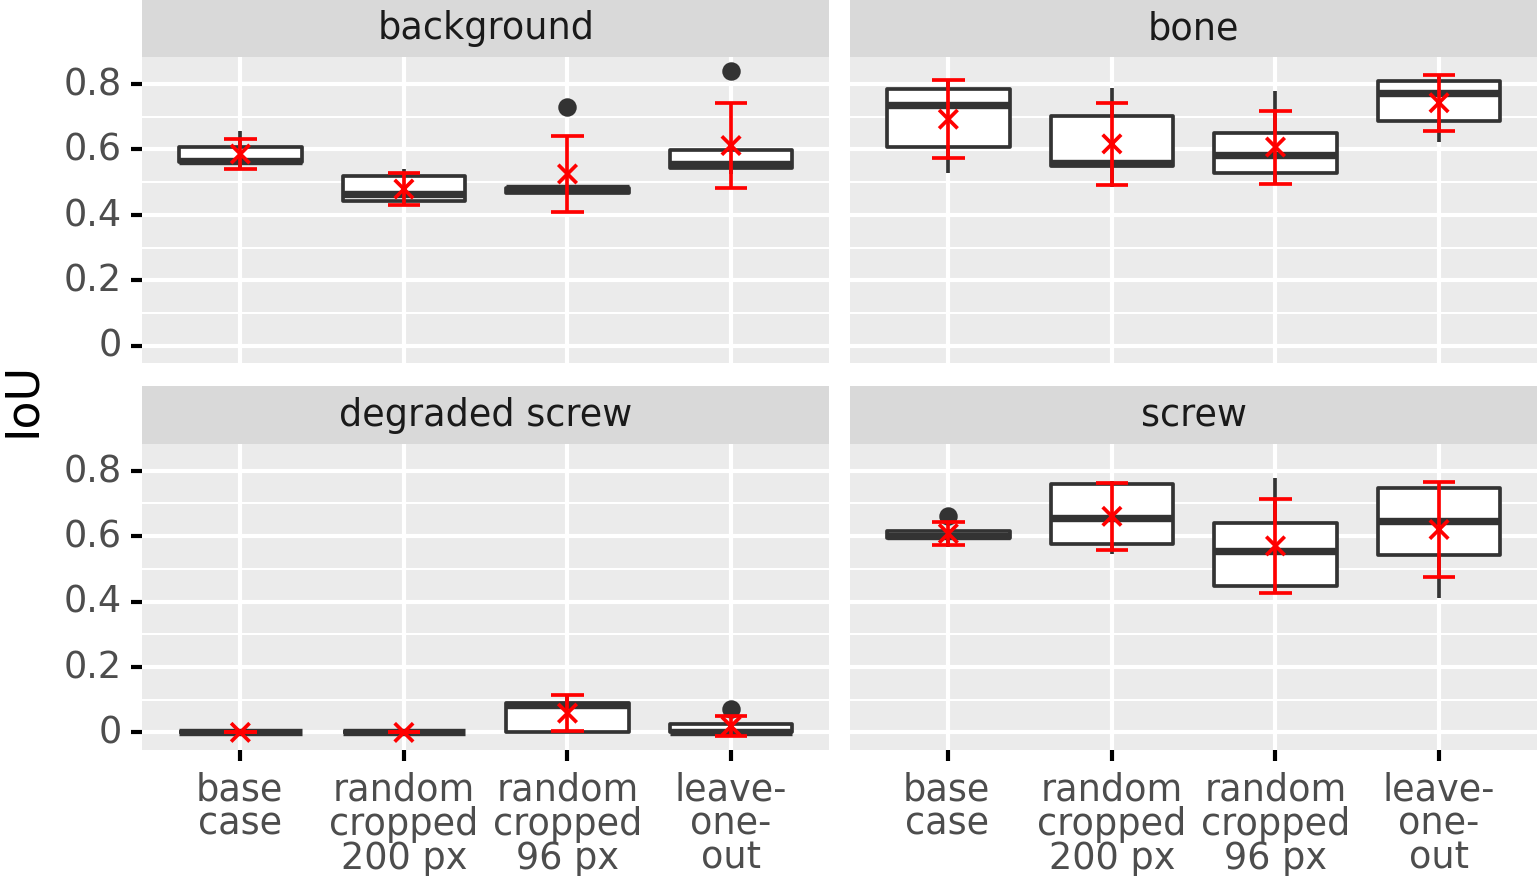
\includegraphics[width=\textwidth]{pictures/experiment_2/compare_all_model_stats_labelwise}\\
    \caption[Labelwise Boxplots of IoU for Best Models]{Boxplots of the IoU for all folds of a configuration. Boxplots indicate the median as solid line, the hinges indicate the inter-quartile range, the whiskers correspond to 1.5 inter-quartile range, and outliers are shown. Additionally, marked in red are mean and standard deviation.}
    %box=50% of data (Inter-Quartile Range (IQR)), line=median, whisker=1.5 IQR, Outliers.
    \label{fig:mIoU-boxplots-labelwise}
\end{figure}


% divergence of folds (and models)
In the random cropping regimes, the folds diverged too\footnote{Additional side-by-side plots of predictions between folds are found in the appendix in~\autoref{subsec:example-predictions-for-cropping-regimes}}, but visually predictions were more similar, as seen in the example predictions of different folds for same image in~\autoref{fig:example-predictions-fold2}.
As seen in \autoref{tab:miou-by-fold}, and visualised in \autoref{fig:accuracy-mIoU-boxplots} and~\ref{fig:mIoU-boxplots-labelwise}, divergence between folds was the same between 200~px random cropped regime and the base case (standard deviation of \gls{miou} between folds was~0.03), and higher in the 96~px random cropped regime, where the standard deviation nearly tripled (to ~0.08).
The standard deviation of \gls{iou} per label between the folds is 0.13~at worst, and 0.03~to~0.04 at best, on all models~(\autoref{tab:miou-by-label}).
Since \formatLabel{degraded screw} was not found in a relevant quantity in any model, the standard deviation is not meaningful for this label.
The divergence is highest for the label \formatLabel{bone} in all models (standard deviation of \gls{iou} of labels~0.10~to~0.11).
Overall, divergence on the 96~px random cropped model is higher in comparison to the other models.
In the label \formatLabel{background}, the standard deviation more than doubled, in \formatLabel{bone}, the standard deviation was more than three times higher than in the base case, while the standard deviation of \formatLabel{bone} stayed nearly the same.

% LOO
A leave-one-out cross-validation was done to investigate this divergence, as especially with small data sets training on more data is often beneficial.
As seen in~\autoref{fig:miou-per-fold}, the leave-one out cross-validation generally behaves more stable than the base case.
The decrease in \gls{iou} is not as pronounced as with five-cold cross validation.
Generally, there was a slight increase in \gls{iou} of the labels (0.02~to~0.05~points \gls{iou}) and also in \gls{miou} (0.03~points), but also often the variability between labels of the same fold increased.
Standard deviation between folds was three to four times higher in most labels, compared to the base case, but the standard deviation of the \gls{miou} was the same~(0.32), and standard deviation of the \gls{miou} nearly tripled to~0.08 in comparison to the base case.
As not all folds of the leave-one-out cross-validation were trained, this metric must be considered with caution, as the other nine folds might still change this significantly.
%LOO: predictions
When considering the predictions of the leave-one-out folds (see~\autoref{fig:example-predictions-folds-loo}), they seem visually very similar to the base case predictions.
Predictions of slices from the edge of the volume and regions outside the sample often are poor, and often the \formatLabel{degraded screw} label is mapped there, as it was also the case in the five-fold cross-validation.

%extra clusters
To further investigate the poor performance of the \formatLabel{degraded screw} label, additional trainings were done with overclustering to allow \gls{stego} to find more clusters than labels and map only the most promising candidates to the labels during validation.
However, as seen in the example predictions (\autoref{fig:example-predictions-fold2}), even with allowing 10~extra clusters, no cluster corresponding to the \formatLabel{degraded screw} label could be found\footnote{Since the evaluation of extra clusters is only done on pixels that were assigned to a ground truth label (not to extra clusters), \gls{miou} values will not be discussed, since they are misleading.}.
But the differentiation of bone and bone marrow, and tissue and sample background improves visibly.

Considering all trained models, even though there is some variability, the best models found are quite similar between folds, and also between different cropping regimes.
This is illustrated in~\autoref{fig:full-example-predictions-slice500}, where the same slice is predicted with each fold of each model.
In some models, areas outside the sample are mapped to different labels (often \formatLabel{degraded screw} or \formatLabel{screw}), but there is no obvious pattern regarding fold or cropping regime.
%All models do predict \formatLabel{screw} quite well, similarly for \formatLabel{bone} and \formatLabel{background}, while no model performs well on \formatLabel{degraded screw}.


\begin{figure}[p]
    \centering
    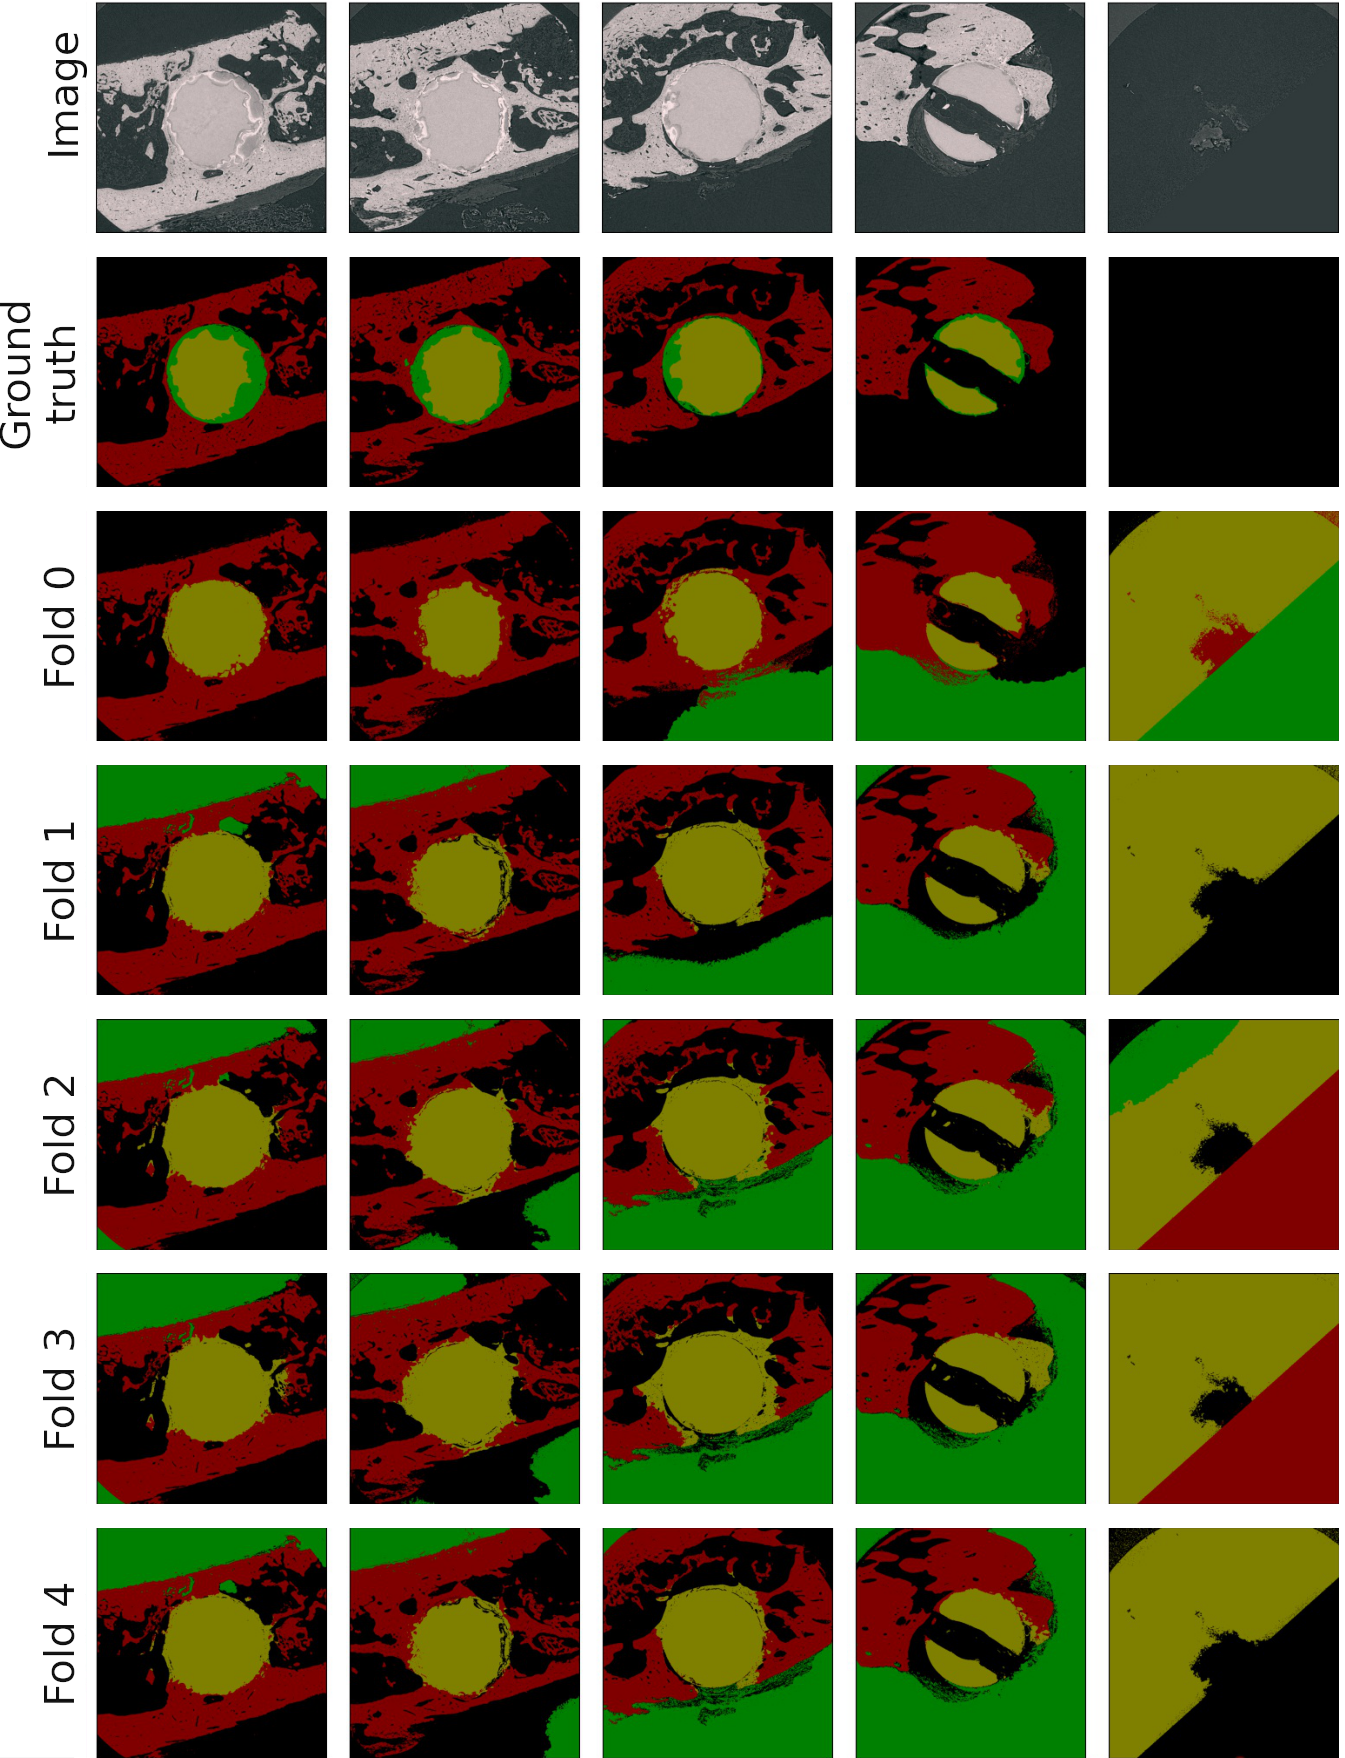
\includegraphics[width=\textwidth]{pictures/experiment_2/for_paper_base-case_final_example_predictions_2_all_folds}\\
    \caption[Foldwise Predictions of the Base Case]{Example predictions of the best models from different folds of the base case. All shown slices belong to the second half of volume syn009HQ (which was neither part of train nor validation set) and are ordered according to spatial location in the volume. Every 100th slice is shown.}
    \label{fig:example-predictions-folds-base-case}
\end{figure}


\begin{figure}[p]
    \centering
    %\vspace{1em}
    \includegraphics[width=\textwidth]{pictures/experiment_2/all_experiments_all_folds_example_predictions2_slice_500}\\
    \caption[Comparison of Predicitons for Same Slice]{Example predictions of the same slice for all best models (all folds). Not shown: leave-one-out cross-validation, since the folds do not correspond. Shown is slice 500 of volume syn009HQ (which was neither part of train nor validation set).}
    \label{fig:full-example-predictions-slice500}
\end{figure}


\begin{figure}[p]
    \centering
    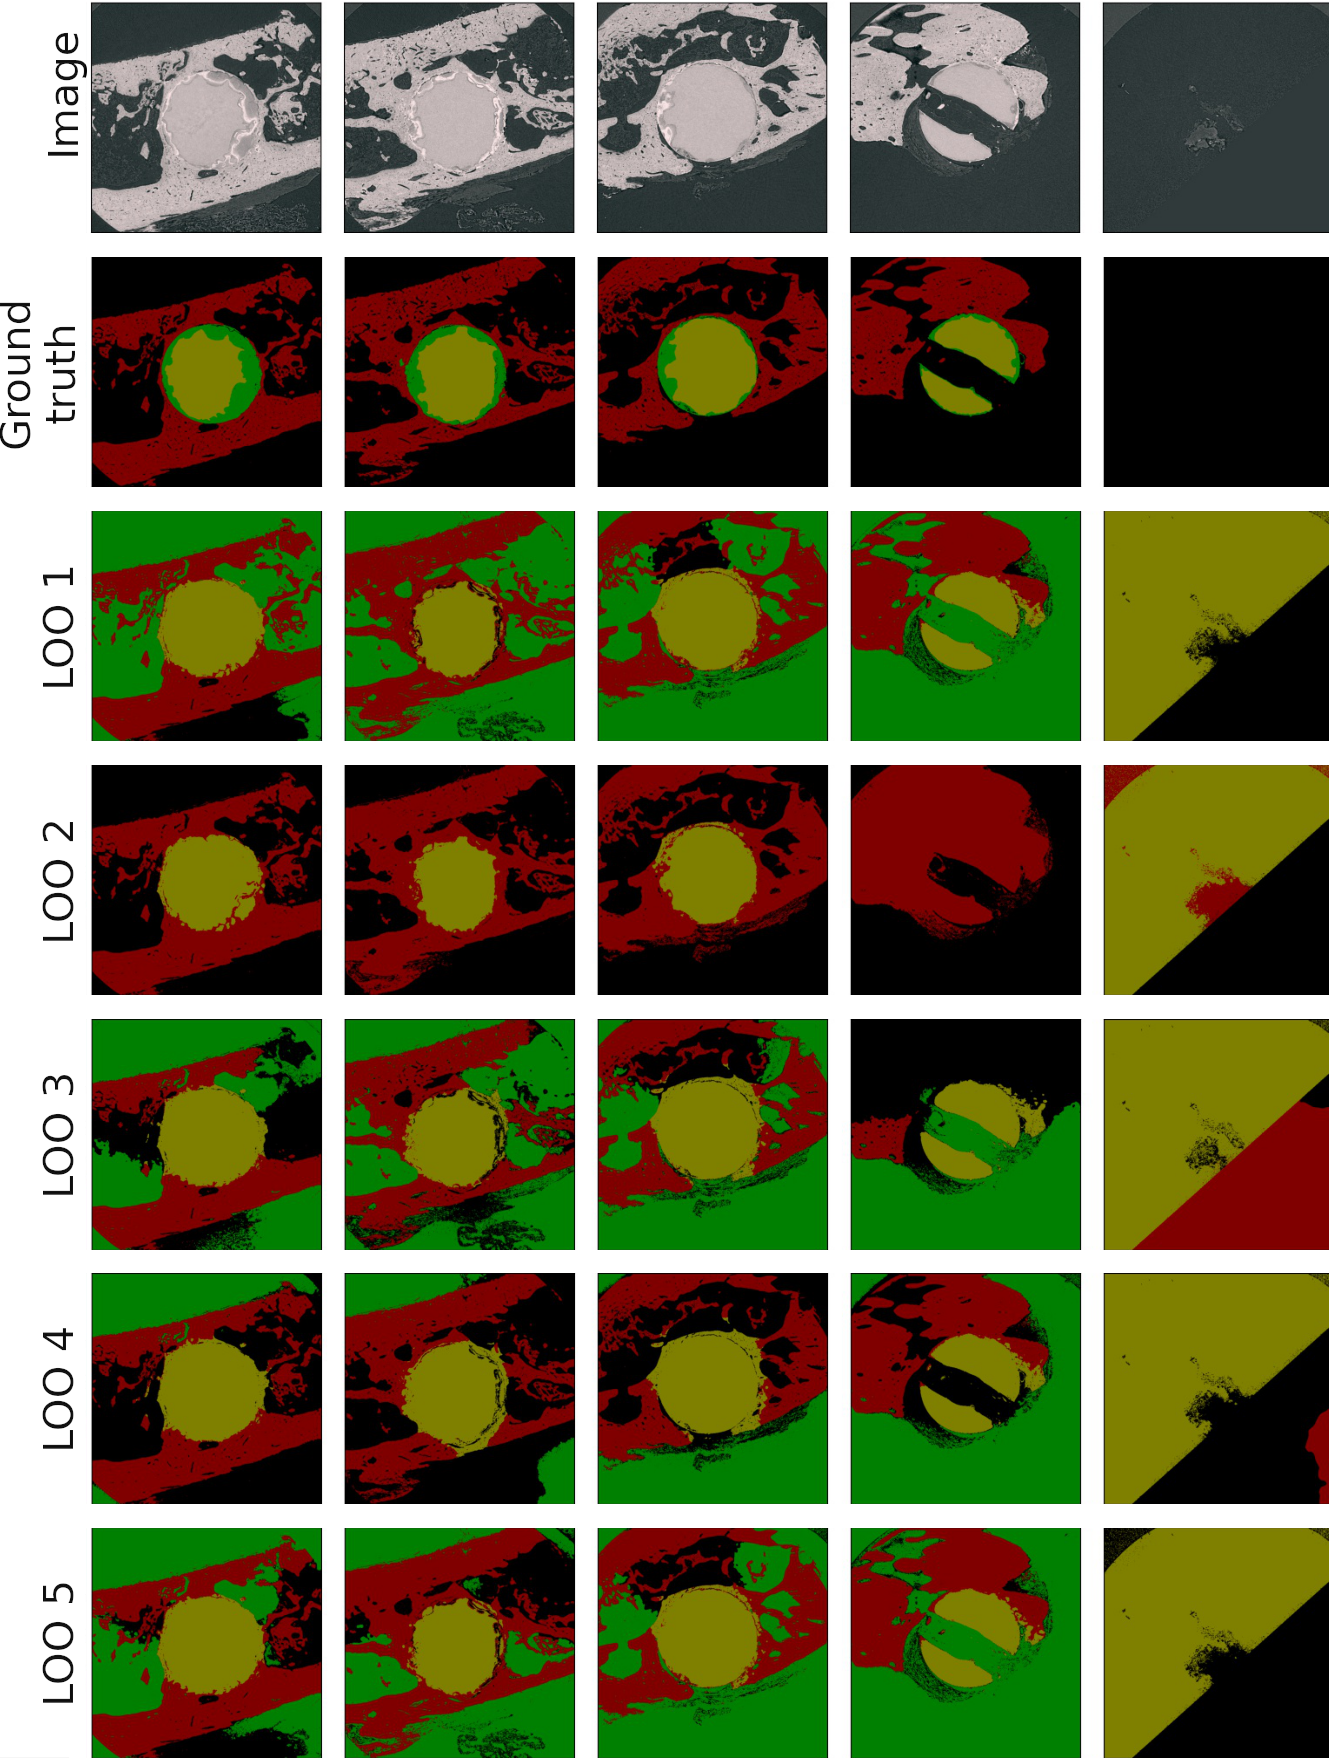
\includegraphics[width=\textwidth]{pictures/experiment_2/for_paper_base-case_LOO_example_predictions_2_all_folds}\\
    \caption[Predictions for Different Leave-one-out Folds]{Example predictions of the best models trained on different leave-one-out folds with all other training configurations the same as for the base case. Folds are labels with LOO (leave-one-out) to indicate that they do differ from the folds seen so far. All shown slices belong to the second half of volume syn009HQ (which was neither part of train nor validation set) and are ordered according to spatial location in the volume. Every 100th slice is shown.}
    \label{fig:example-predictions-folds-loo}
\end{figure}

\begin{figure}[p]
    \centering
    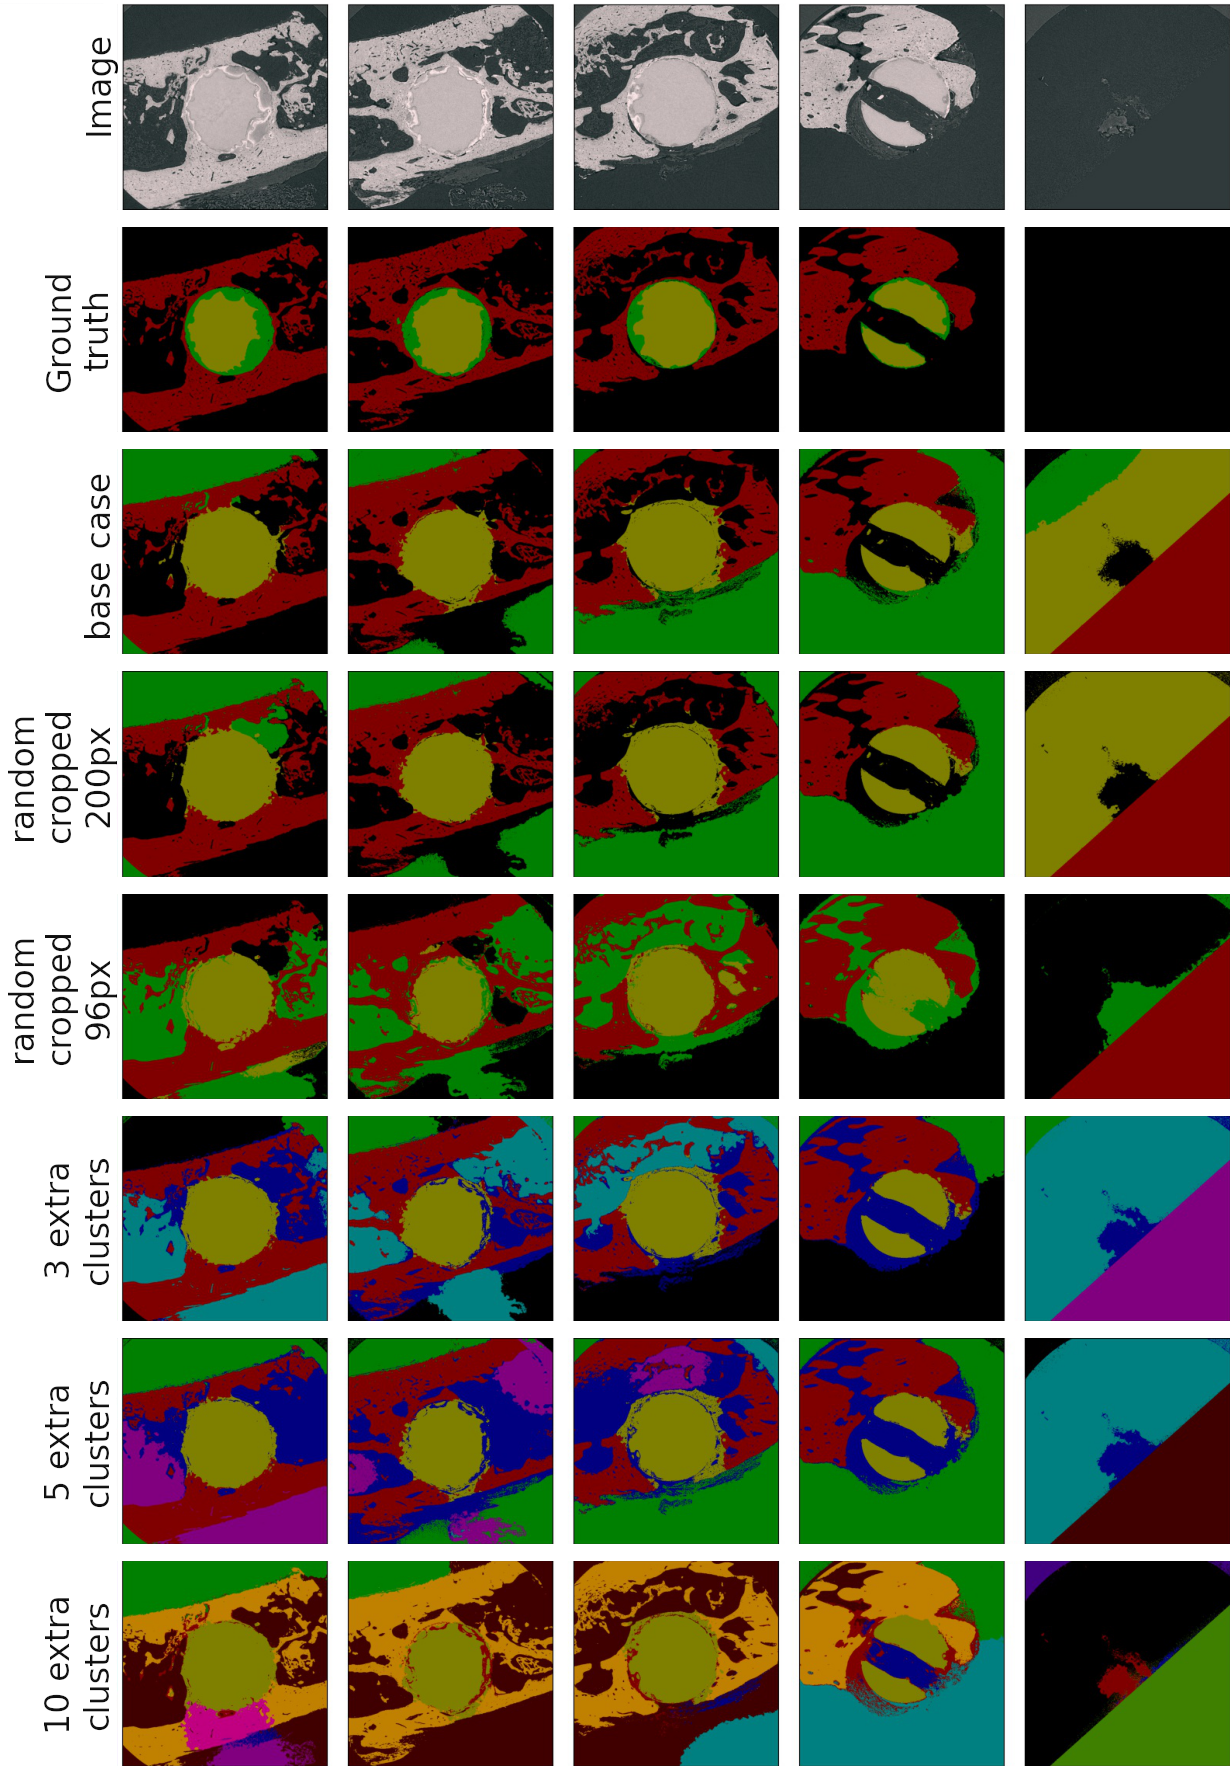
\includegraphics[width=\textwidth]{pictures/experiment_2/for_paper_all_experiments_example_predictions_2_Fold2}\\
    \caption[Comparison of Predictions for Same Fold]{Example predictions of Fold 2 of the base case, random cropping regimes, and overclustering regimes. For the overclustering regimes, the number of extra clusters is given. All shown slices belong to the second half of volume syn009HQ (which was neither part of train nor validation set) and are ordered according to spatial location in the volume. Every 100th slice is shown.}
    \label{fig:example-predictions-fold2}
\end{figure}
% contain the floats in this subsection
\FloatBarrier

\subsection{Discussion}
In this section, experiments will be discussed separately, followed by a comparison of results and a discussion of the potential of \gls{stego} for segmentation of scientific images.

\subsubsection{Experiment 1: Predict with Provided Models}
As expected, the pre-trained models did not perform well.
However, some resolution could be reached with all models, especially for \formatLabel{background}, where \gls{miou} was between 0.6 and 0.7.

%Potsdam
Potsdam only did a binary differentiation of \formatLabel{screw/degraded screw} from everything else.
However, even this separation is not distinguished very well, since often some nooks belonging to the bone and bone marrow are included (false positives).
The screw, in contrast, is always fully included in the label, no part is missing (few false negatives).
On the other hand, it does remarkably well on distinguishing the cracks in the screw, as seen in the example segmentations (\autoref{fig:pretrained-predictions}).
Overall, if the task was to only segment \formatLabel{screw/degraded screw} vs. \formatLabel{background}, this model would be not bad.
This means, that in the image features received from the backbone, there is something included, that can be used to identify screws.
%Potsdam was trained on aerial images, which are (in contrast to photographies on which the other models were trained), more similar to SRµCT pictures. So this might explain, why it performs better on the more laminary \formatLabel{screw} label.

% Cocostuff
With COCO-Stuff, most clusters mapped to the background of the sample, thus mostly \formatLabel{background} is predicted, with some segments of \formatLabel{bone} also identified correctly.
When \formatLabel{bone} was identified, it was usually correct, meaning that not many false positives were found.
However, \formatLabel{bone} was identified only where the depicted bone had a lighter color (a higher pixel value) and was very homogenous in the image, indicating that mostly pixel values were utilised for prediction.
%manual clustering
With the manual assignment of cluster 5 to \formatLabel{bone}, COCO-Stuff predictions did resemble the Cityscapes model more (in \gls{miou} as well as visually).
The biggest difference between these models then was, that COCO-Stuff yields more laminar clusters, with \formatLabel{bone} encompassing the full bone including matrix and screw, while the Cityscapes prediction is much more ragged and often neatly follows the lines of the bone marrow.


%Cityscapes
With Cityscapes, \formatLabel{background} and \formatLabel{bone} yielded similar \gls{miou} as predictions with COCO-Stuff.
However, as shown in the images, \formatLabel{bone} did correlate with the ground truth shape to a higher degree, which might indicate that only the border pixels differed.
As this might even be the case between two experts assigning the ground truth labels~\autocite{Webb2021}, the \gls{miou} might not be the best metric to choose for a comparison.
And as discussed in~\autocite{Reinke2022}, \gls{miou} especially is disadvantageous with close matches, since it does not differentiate between divergence at borders of regions or completely separate regions (for more details see~\autocite{Reinke2022}).
So overall, the Cityscapes model should be considered more effective than COCO-Stuff and also better than Potsdam at distinguishing \formatLabel{bone} from \formatLabel{background}, while Potsdam is more efficient at identifying \formatLabel{screw}.

% compare to paper results
In comparison to the model performance on the validation sets of the pre-trained models, it stands out that~–~with respect to \gls{miou}~–~the predictions on the screws data set are nearly as good as the validation results presented in the paper~\autocite{Hamilton2022}.
That means, prediction with an arbitrary selected model yielded similar results as predictions on the validation set of that model in terms of \gls{miou}.
However, when considering the actual predictions, it shows that they are very ineffective in comparison to the predictions of the validation set of the model.
Roughly the same proportions of pixels are in fact classified correctly as indicated by \gls{miou}, but especially borders between labels are often off, thus rendering the whole prediction pointless.
In comparison, the results on the original validation set do look more promising~\autocite{Hamilton2022}.
There, labels can be distinguished quite well and borders between labels often match at least in a broad sense~\autocite{Hamilton2022}.
This once again highlights the often deficient expressiveness of the \gls{miou}, as no differentiation is made between border pixels and others.
A more thorough discussion of the ~\gls{miou} (and other metrics) can be found in~\autocite{Reinke2022}.

% combination?
In combination, Potsdam and Cityscapes might yield acceptable results for the labels \formatLabel{background, bone}, and \formatLabel{screw} (e.g. by predicting after each other and merging \formatLabel{screw} pixels of Potsdam into \formatLabel{bone} pixels of Cityscapes).
However, a more promising approach would probably be to just train a new model for the screws data set.

% contain the floats in section
\afterpage{\FloatBarrier}

\subsubsection{Experiment 2: Train on Scientific Data Set}\label{subsubsec:discussion-experiment2}
In the following, the performance of the training regimes will be evaluated and compared to each other, as well as to the predictions made with the pre-trained models in experiment 1.
Especially the divergence between folds will be discussed, as well as the poor performance on the \formatLabel{degraded screw} label.
Eventually, recommendations for training \gls{stego} will be addressed.

%weight selection/tuning
As explained earlier, \gls{stego} requires six parameters of the loss function to be tuned depending on the training data used.
Tuning was done based on the recommendations by \gls{stego}s authors.
This means, the cosine distance signales were tuned to reach two distinct positive and negative signals, as illustrated in the segmentation correspondence histograms provided during training~\autocite{Hamilton2022}.
Originally, it was recommended to balance these signals to generate separated signals of approximately the same strength.
However, it turned out that slightly increasing the negative signal worked best for the used data, regardless of cropping regime and resolution\footnote{The full list of used parameters is found in \autoref{tab:training-parameters}.}.
A reason for this might be, that since the data set is very homogenous, with most slices showing the same view of the same objects over and over again, there is an imbalance in positive and negative signals.
Plenty of positive signal was provided from the similar images, but especially negative signal was rare.
That might be the reason why artificially shifting this balance towards negative signals was helpful.

% overall model performance
Overall, the models performed well, apart from the \formatLabel{degraded screw} label.
The differences between folds were minor.
Predictions on the validation set tend to be very similar: all models predict \formatLabel{bone} quite well, same goes for \formatLabel{screw} and \formatLabel{background}, while no model performs well on \formatLabel{degraded screw}.
The consistently poor performance of \formatLabel{degraded screw} highlights once again the challenging task to differentiate \formatLabel{degraded screw} from \formatLabel{screw}.
Since this label is so scarce, performance would considerably increase, when excluding \formatLabel{degraded screw} from the calculation of \gls{miou}.
This is impressively shown by the accuracy values, which are consistently higher than the \gls{miou} values, since they indicate the overall proportion of correctly classified pixels, while \gls{miou} is calculated as mean over labels, where all labels contribute equally.

% compare to predictions with pre-trained models
This relatively good performance of the models also shows in comparison with the predictions made with the pre-trained models, as the \gls{miou} nearly doubled.
Even though there were some labels, that did perform quite well in regard to \gls{iou} in the pre-trained models (for example \formatLabel{background}, where \gls{iou} was between 0.69 and 0.71), these predictions were far from good.
For example, the COCO-Stuff model, which yielded a \gls{iou} of 0.69 on \formatLabel{background}, nearly always predicted \formatLabel{background}.
So, the differentiating capacities were poor.\footnote{This again highlights the shortcomings of using the \gls{iou} as single metric for model evaluation (as discussed in~\autocite{Reinke2022}.}
Thus overall, it can be confirmed that training the segmentation head for specific tasks is beneficial and significantly improved model quality in comparison to arbitrary selected models.
However, the results for scientific data are still not satisfactory to be used in real-world scenarios.


% divergence of folds (and models)
As mentioned earlier, the development of the \gls{miou} diverges between folds in all trainings.
This might be attributed to the fact, that too few training examples were used, or that the models were not sufficiently tuned.
In the future, a more thorough parameter tuning should be done, possibly using grid search algorithms to find better parameters.
To investigate influence of data availability, training with the base case configuration was also done on five folds of a leave-one-out cross-validation.\footnote{Since it already showed, that divergence is present in a leave-one-out setting, too, training was stopped after five folds.}
%LOO
However, as seen in~\autoref{fig:miou-per-fold}, the divergence between folds was found in the leave-one-out cross-validation as well.
This indicates a higher variance between folds in the leave-one-out case, as it is often the case, when training sets are highly correlated~\autocite{Bengio2004}.
Overall, using a leave-one-out cross-validation did not improve model quality significantly.

%extra clusters
When overclustering was done, it was found that differentiation between bone and bone marrow, as well as between background and soft tissue, did improve visibly.
This is insofar remarkable, as this differentiation is not made in the ground truth, which highlights the potential of unsupervised algorithms, which are able to derive structures independently of the ground truth provided.

Concerning the \formatLabel{degraded screw} label, however, this label could not be retrieved, even when allowing for ten extra clusters.
Thus, it can be assumed, that at the current state of \gls{stego}, it seems not to be possible to retain this challenging label.
As \formatLabel{degraded screw} only slightly differs from \formatLabel{screw} in regard of absorption (and thus pixel values) or texture, it might be the case, that the feature vectors derived form the backbone did not differentiate these enough (meaning the feature embeddings are too similar to be clustered separately).
Thus, switching the backbone to something adapted for \gls{srmct} images should definitively be done in the future, to see if this helps feature embedding.
At least in principle, differentiating \formatLabel{screw} and \formatLabel{degraded screw} should be possible, as the \formatLabel{degraded screw} label has been successfully retained in another study~\autocite{Baltruschat2021}, which indicates, that there is something in the data, that can be used for differentiation (and it is very unlikely that it is just the label, that differentiates it).

%compare with supervised prediction
In comparison to this study~\autocite{Baltruschat2021}, which was done on the same data set, the results achieved here are worse.
However, it has to be noted, that the study was done with a supervised Network (a U-net), and also utilised 3D fusing, meaning predictions were done from multiple directions and combined by probability~\autocite{Baltruschat2021}.
Still, even without 3D fusing, results were significantly better: labels reached around 0.90~\gls{iou}, and even the \formatLabel{degraded screw} label reached 0.80~\autocite{Baltruschat2021}.

% very good for unsupervised
However, even though results are not ready to be used in a scientific real-world application, in the context of unsupervised segmentation, the achieved result is very good.
Most other unsupervised segmentation algorithms tend to reach a \gls{miou} of 0.12~to~0.31 (depending on the data set)~\autocite{Cho2021}, 0.21~\autocite{Hamilton2022}, or at best~0.50~to~0.63 (depending on number of classes)~\autocite{VanGansbeke2021} on default (2D) image data sets.

% RESULT: How to train SRµCT data?
The remaining problem to be solved is, that no clear recommendation regarding the cropping scheme could be derived from the experiments presented, due to the divergence during cross validation.
Overall, the base case was found to perform slightly better than the random cropped regimes in regard to \gls{miou}, which was 0.47 (mean over folds), single folds even reached scores of 0.49 or 0.50.
The base case was also found to yield the best \gls{miou} scores (mean over folds) for \formatLabel{background} and \formatLabel{bone} (0.59 and 0.69 respectively) and the second best for \formatLabel{screw} (0.61)\footnote{Leave-one-out cross-validation is excluded from this comparison, since not all folds were trained.}.
It also did diverge less between folds.
But again, these differences were only minor compared to the other cropping regimes, and similar differences between models were even found between folds of the base case.
However, all models were able to predict the labels to some degree.
Finally, this means, that the idea of a heterogeneous data set (as generated through random cropping) being more beneficial when training \gls{stego}, could not be confirmed.
Since results of all trainings are very similar regarding the final model and training times until the best model is found, did not differ a lot (1.5~to 5~hours), there is no definite answer to which cropping regime and resolution to prefer.
As the \gls{miou} curves of the random cropped regimes do not fluctuate as much (and especially performance does not decrease as much over time), it might be preferred over the base case.
Especially, since it can be suspected that these trainings might even improve with further training (for example fold~1 on 96~px random cropped,~\autoref{fig:miou-per-fold-label}), random cropping might be advantageous, as training these for longer still results in reasonable training times (20 epochs took only 4.5~h and 1.5~h).


\subsubsection{Potential of STEGO for Scientific Segmentation}
% compare to stegos performance on default sets and wrap up
In a broader view, it is remarkable how well \gls{stego} performed on the \gls{srmct} data, for which it was never designed.
When comparing the results with those of the original trainings done on photography based data sets, the \gls{miou} nearly doubled.
This might largely be attributed to the fact, that through training on very similar images, which always depict the same object, the number of training examples per label is very high.
But given that \gls{stego} was used for scientific segmentation, which it was not designed for, and with a backbone that was also not designed for scientific images, the results are very good.
Achieving these promising results with such an unsuitable backbone highlights the potential \gls{stego} has to be adapted for unsupervised semantic segmentation of scientific images.


\subsubsection{Future Work}
This paper does only provide a very broad evaluation of \gls{stego}.
Especially to give better recommendations for training \gls{stego} on scientific images, more research is needed.

% train backbone
The factor that probably has the most influence is the backbone, which was frozen and not trained in any capacity.
This backbone was originally trained on photographs~\autocite{Hamilton2022,Caron2021} and was not adjusted for ~\gls{srmct} images.
As stated in~\autocite{Cheplygina2019}, even though ImageNet is often used in transfer learning set-ups for medical images, this is largely attributed to its availability, as there are only few alternative so readily available.
Even though correlation correspondence was promising (as shown in~\autoref{fig:correspondencemap-screws}), training the backbone specifically on \gls{srmct} data might significantly enhance feature embedding of the output, which in turn should be easier to cluster by the segmentation head.
So in the long run, it should be investigated, if training the backbone enhances results.

% parameter tuning
Additionally, a systematic grid search to optimise training parameters might also improve the results.
There could even be parameter combinations, that mitigate the divergence between folds or significantly improve resolution of the \formatLabel{degraded screw} label.
% more data
%In that regard, trainings done on more data can also be helpful.

% other grey value normalisation
Also the used pixel-value normalisation scheme should be investigated further, since the used scheme still relies on mean and standard deviation derived from photographs.
Adapting the normalisation scheme to the respective imaging modality could also enhance the feature quality derived from the backbone.

%% other modalities
Generally, working with more and different data should also be evaluated, since a single \gls{srmct} data set is not representative for scientific imaging at all.
Even combining different data sets of both the same and different imaging modalities to enhance data and label heterogeneity might help.
%stegos potential is not fully utilised in this study
And it was not even tried in this study to utilise the 3D information embedded in the data set.
Future research might aim at integrating the 3D aspect, for example by using slices from different directions for training and combining final 3D predictions from single slice predictions of different directions, as done in~\autocite{Zhou2017}.


\section{Conclusions}\label{sec:conclusions}
%setting and problem
Scientific imaging plays a major role in many clinical applications and biomedical studies.
However, image segmentation is a time-consuming process when done manually, and often experts are needed to identify structures correctly~\autocite{Litjens2017}.
But even when automatic segmentation algorithms are used, at least some manual segmentations are needed, since to date all state-of-the-art algorithms for scientific image segmentation are supervised and rely on annotated training data~\autocite{Litjens2017}.
The aim of this project thus was to adapt an unsupervised algorithm \gls{stego}~\autocite{Hamilton2022} to be used with high-resolution scientific imaging data and evaluate this method on a scientific imaging data set (depicting degradation of screws in bones).

% solution we found
It was shown that \gls{stego} can be used with scientific data, and specifically training a model on a data set significantly improved predictions in comparison to an arbitrary (pre-trained) model.
%lessons learned
%problems
However, the resulting predictions can not yet be used in a real-world science context.
Particularly one label (\formatLabel{degraded screw}) was not detected at all rate, which might hint at the fact that the features received from the backbone might not embed this label well.
Moreover, because the divergence between cross-validation folds was similar to divergence between training configurations, no clear suggestions regarding training configurations for scientific data could be derived.
%next steps
To mitigate these shortcomings, the next steps should include a grid search for better training parameters, and training the backbone (which was adjusted for photographs, not scientific images), to reach a better feature embedding.

%findings and potential
Given that \gls{stego} is an unsupervised algorithm, results are impressive, as explained earlier.
Additionally, it must be considered that unsupervised algorithms identify structures in the data, that do not necessarily align with the structures that were represented in the ground truth.
So aberration from the ground truth has to be expected to some degree.
And given that \gls{stego} was used for scientific segmentation, which it was not designed for, the results are very encouraging. % with a backbone that was also not designed for scientific images,
Achieving these promising results highlights the potential of \gls{stego} to be further adapted in the future for unsupervised semantic segmentation of scientific images.

% so footnotes are placed reasonably
\clearpage 

\printbibliography[heading=bibnumbered]


\clearpage
\pagenumbering{roman}
\clearpage
\newpage
% also set appendices to new page
%\addtocontents{toc}{\protect\newpage} #todo to shift appendix in toc on new page
\appendix      %is not resetting counters?
\section*{Appendix}
\addcontentsline{toc}{section}{Appendix}
\addtocontents{toc}{\protect\addtolength{\protect\cftsubsecnumwidth}{10pt}} % form here on add space in toc between number and name of section must be increased, because of roman numrals
\renewcommand\thesubsection{A.\Roman{subsection}}

% redefine names for floats (prepend A.)
\renewcommand\thefigure{A.\arabic{figure}}   
\renewcommand\thetable{A.\arabic{table}}
\renewcommand\thelstlisting{A.\arabic{lstlisting}} 
% reset counters
\setcounter{figure}{0}                        
\setcounter{table}{0}
\setcounter{lstlisting}{0} 

\subsection{Persisting Issues of STEGO}\label{subsec:stego-persisting-issued}
\begin{itemize}
    \item The hardcoded properties of default datasets should instead be placed in configuration files.
    This is a design issue and does not influence results.
    \item When executing the evaluation procedure, the comparison with \gls{picie}~\autocite{Cho2021} is not possible (a class not found error is thrown).
    This is because of implementation flaws that cannot be fixed easily, but is only relevant for this comparison.
    \item A benign RuntimeWarning concerning the C header of numpy is issued by Cython, which is usually silenced in the numpy-init function, but silencing happens do be removed in the numpy version in the \gls{stego} environment. Since the environment could not be altered, this warning is just ignored. For more details on this warning see the discussion on github~\autocite{rgommers2012}.
    %".../lib/python3.6/importlib/_bootstrap.py:219: RuntimeWarning: numpy.ufunc size changed, may indicate binary incompatibility. Expected 192 from C header, got 216 from PyObject"
    % no problem: https://stackoverflow.com/questions/40845304/runtimewarning-numpy-dtype-size-changed-may-indicate-binary-incompatibility
    \item DDP warnings are issued ``Grad strides do not match bucket size''.
    This may only impair performance, but not results.
    \item A torch warning is issued because ``compute method'' is called before ``update method''.
    Since the compute method is only called to tell \tensorboard{} to monitor this metric in the future, this is not a problem.
    \item CropComputer class should not be a dataset, but get and adjust a dataset.
    This is a design issue and does not influence results.
\end{itemize}

\clearpage

\clearpage
\subsection{Screws Predictions with Pre-trained Models}
\begin{figure}[!htb]
    \centering
    \includegraphics[clip,trim={0 0 0 36}, height=\textwidth, angle=90]{pictures/experiment_1/pretrained-models_cluster-predictions_example_predictions_2_all}\\
    \caption[Predictions from Provided Models]{Predictions from provided models. Visualisation of image, ground truth, raw cluster predictions and clusters combined by most likely match to ground truth label. Raw cluster colors correspond to cluster names in~\autoref{fig:correlation-matrix-pretrained}. All shown slices belong to volume syn009HG and are ordered according to spatial location in the volume. Every 100th slice is shown. Image rotated by 90~degree.}
    \label{fig:pretrained-predictions_syn009}
\end{figure}
\clearpage

\subsection{Cross-validation of Screws Data Set}\label{subsec:cross-validation-screws}
\begin{table}[!htb]
    \centering
    \makegapedcells
    \begin{tabular}{|c|p{0.62\textwidth}|p{0.2\textwidth}|}
        \hline
        \textbf{Fold} & \textbf{Train set} &\textbf{Validation~set} \\
        \hline
        0 & 113731Mg10, syn018, syn020, syn021, syn022, syn026, syn030, syn032, syn033, syn038, syn041 & 113724Mg10, 113726Mg5, 113728Mg10 \\
        \hline
        1 & 113724Mg10, 113726Mg5, 113728Mg10, syn021, syn022, syn026, syn030, syn032, syn033, syn038, syn041 & 113731Mg10, syn018, syn020 \\
        \hline
        2 & 113724Mg10, 113726Mg5, 113728Mg10, 113731Mg10, syn018, syn020, syn030, syn032, syn033, syn038, syn041 & syn021, syn022, syn026 \\
        \hline
        3 & 113724Mg10, 113726Mg5, 113728Mg10, 113731Mg10, syn018, syn020, syn021, syn022, syn026, syn038, syn041 & syn030, syn032, syn033 \\
        \hline
        4 & 113724Mg10, 113726Mg5, 113728Mg10, 113731Mg10, syn018, syn020, syn021, syn022, syn026, syn030, syn032, syn033 & syn038, syn041 \\
        \hline
        \hline
        {\small LOO} 1 & 113731Mg10, 113724Mg10, 113728Mg10, syn018, syn020, syn021, syn022, syn026, syn030, syn032, syn033, syn038, syn041 & 113726Mg5 \\
        \hline
        {LOO} 2 &  113731Mg10, 113724Mg10, 113726Mg5, syn018, syn020, syn021, syn022, syn026, syn030, syn032, syn033, syn038, syn041& 113728Mg10\\
        \hline
        {LOO} 3 &  113724Mg10, 113726Mg5, 113728Mg10, syn018, syn020, syn021, syn022, syn026, syn030, syn032, syn033, syn038, syn041 &  113731Mg10\\
        \hline
        { LOO 4} & 113731Mg10, 113724Mg10, 113726Mg5, 113728Mg10,syn020, syn021, syn022, syn026, syn030, syn032, syn033, syn038, syn041 &  syn018\\
        \hline
        { LOO 5} &   113724Mg10, 113726Mg5, 113728Mg10, 113731Mg10, syn018, syn021, syn022, syn026, syn030, syn032, syn033, syn038, syn041 & syn020\\
        \hline
        %\makecell{\textbf{Test set}\\\textbf{Exp. 1}} & \multicolumn{2}{c|}{113734HQMg5, syn009HQ, 113729HQMg5} \\
        %\hline
    \end{tabular}
    \caption[Cross-validation Sets of Screws Data Set]{Cross-validation sets of screws data set. For each fold volumes names for train and validation set are given. Folds of the leave-one-out cross-validation are marked with ``LOO'' to indicate difference from the five-fold cross-validation folds.} % Since the number of volumes is not a multiple of 5 the last fold of the five-fold cross-validations only contains two volumes in the validation set. 
    \label{tab:folds-screws}
\end{table}

\clearpage
\subsection{Parameters Used for Training}
\begin{table}[!htb]
    \centering
    \makegapedcells
    \begin{tabular}{|c|r|>{\raggedleft\arraybackslash}p{0.19\textwidth}|>{\raggedleft\arraybackslash}p{0.19\textwidth}|}
        \hline
        \makecell{\textbf{Parameter}} & \makecell{\textbf{Base-case,}\\ \textbf{extra clusters}} & \makecell{\textbf{Random} \\ \textbf{cropped} \\ \textbf{(200~px)}} & \makecell{\textbf{Random} \\ \textbf {cropped} \\ \textbf{(96~px)}} \\
        \hline
        \makecell{ $\lambda_{rand}$ \\ neg\_inter\_weight} & 0.4 & 0.4 & 0.4 \\ \hline
        \makecell{ $\lambda_{knn}$ \\pos\_inter\_weight} & 0.2 & 0.2 & 0.2 \\ \hline
        \makecell{ $\lambda_{self}$ \\pos\_intra\_weight} & 0.4 & 0.4 & 0.4 \\ \hline
        \makecell{$b_{rand}$\\neg\_inter\_shift} & 0.85 & 0.55 & 0.5 \\ \hline
        \makecell{$b_{knn}$\\pos\_inter\_shift} & 0.45 & 0.45 & 0.4 \\ \hline
        \makecell{$b_{self}$\\pos\_intra\_shift} & 0.35 & 0.35 & 0.55 \\ \hline
    \end{tabular}
    \caption[Training Parameters]{Parameters Used for Training. For each of the trainings the six manually selected parameters are given. Each parameter is named by their configuration file name as well as the corresponding name in \gls{stego} paper. Parameters where tuned according to recommendations from \gls{stego}s authors, with minor changes, as explained in~\autoref{subsubsec:discussion-experiment2}.}
    \label{tab:training-parameters}
\end{table}


\clearpage
\subsection{Runtimes of Experiments}
\begin{table}[!htb]
\centering
\makegapedcells
\begin{tabular}{|l|l|r|}
    \hline
    \textbf{Experiment} & \textbf{Description} & \textbf{Runtime} \\
    \hline
    Exp. 1 & Prediction with Potsdam model & $\approx$ 5.25~hours\\ \hline
    Exp. 1 & Prediction with Cocostuff model & $\approx$ 11.75~hours\\ \hline
    Exp. 1 & Prediction with Cityscapes model & $\approx$ 12.25~hours\\ \hline
    \hline
    Exp. 2 & \makecell[l]{Train base-case\\batch size: 8} & $\approx$1.25~days\\ \hline
    Exp. 2 & \makecell[l]{Train extra clusters\\batch size: 8} & $\approx$1.25~days\\ \hline
    Exp. 2 & \makecell[l]{Train random cropped (200~px)\\batch size: 16} & $\approx$4.5~hours\\ \hline
    Exp. 2 & \makecell[l]{Train random cropped (96~px)\\batch size: 32} & $\approx$1.5~hours\\ \hline
    Exp. 2 & \makecell[l]{Train base-case leave one out\\batch size: 8} & $\approx$1.5~days\\ \hline
\end{tabular}
\caption[Runtimes of Experiments]{Runtimes of experiments. Each experiment was run on a computation node, containing four V100 GPUs. For the predictions total run time is given. For the trainings approximate runtime for one fold and the batch size is given.}
\label{tab:runtimes}
\end{table}

\clearpage
\subsection{Fold- and Label-wise Development of IoU}
\begin{figure}[!htb]
    \centering
    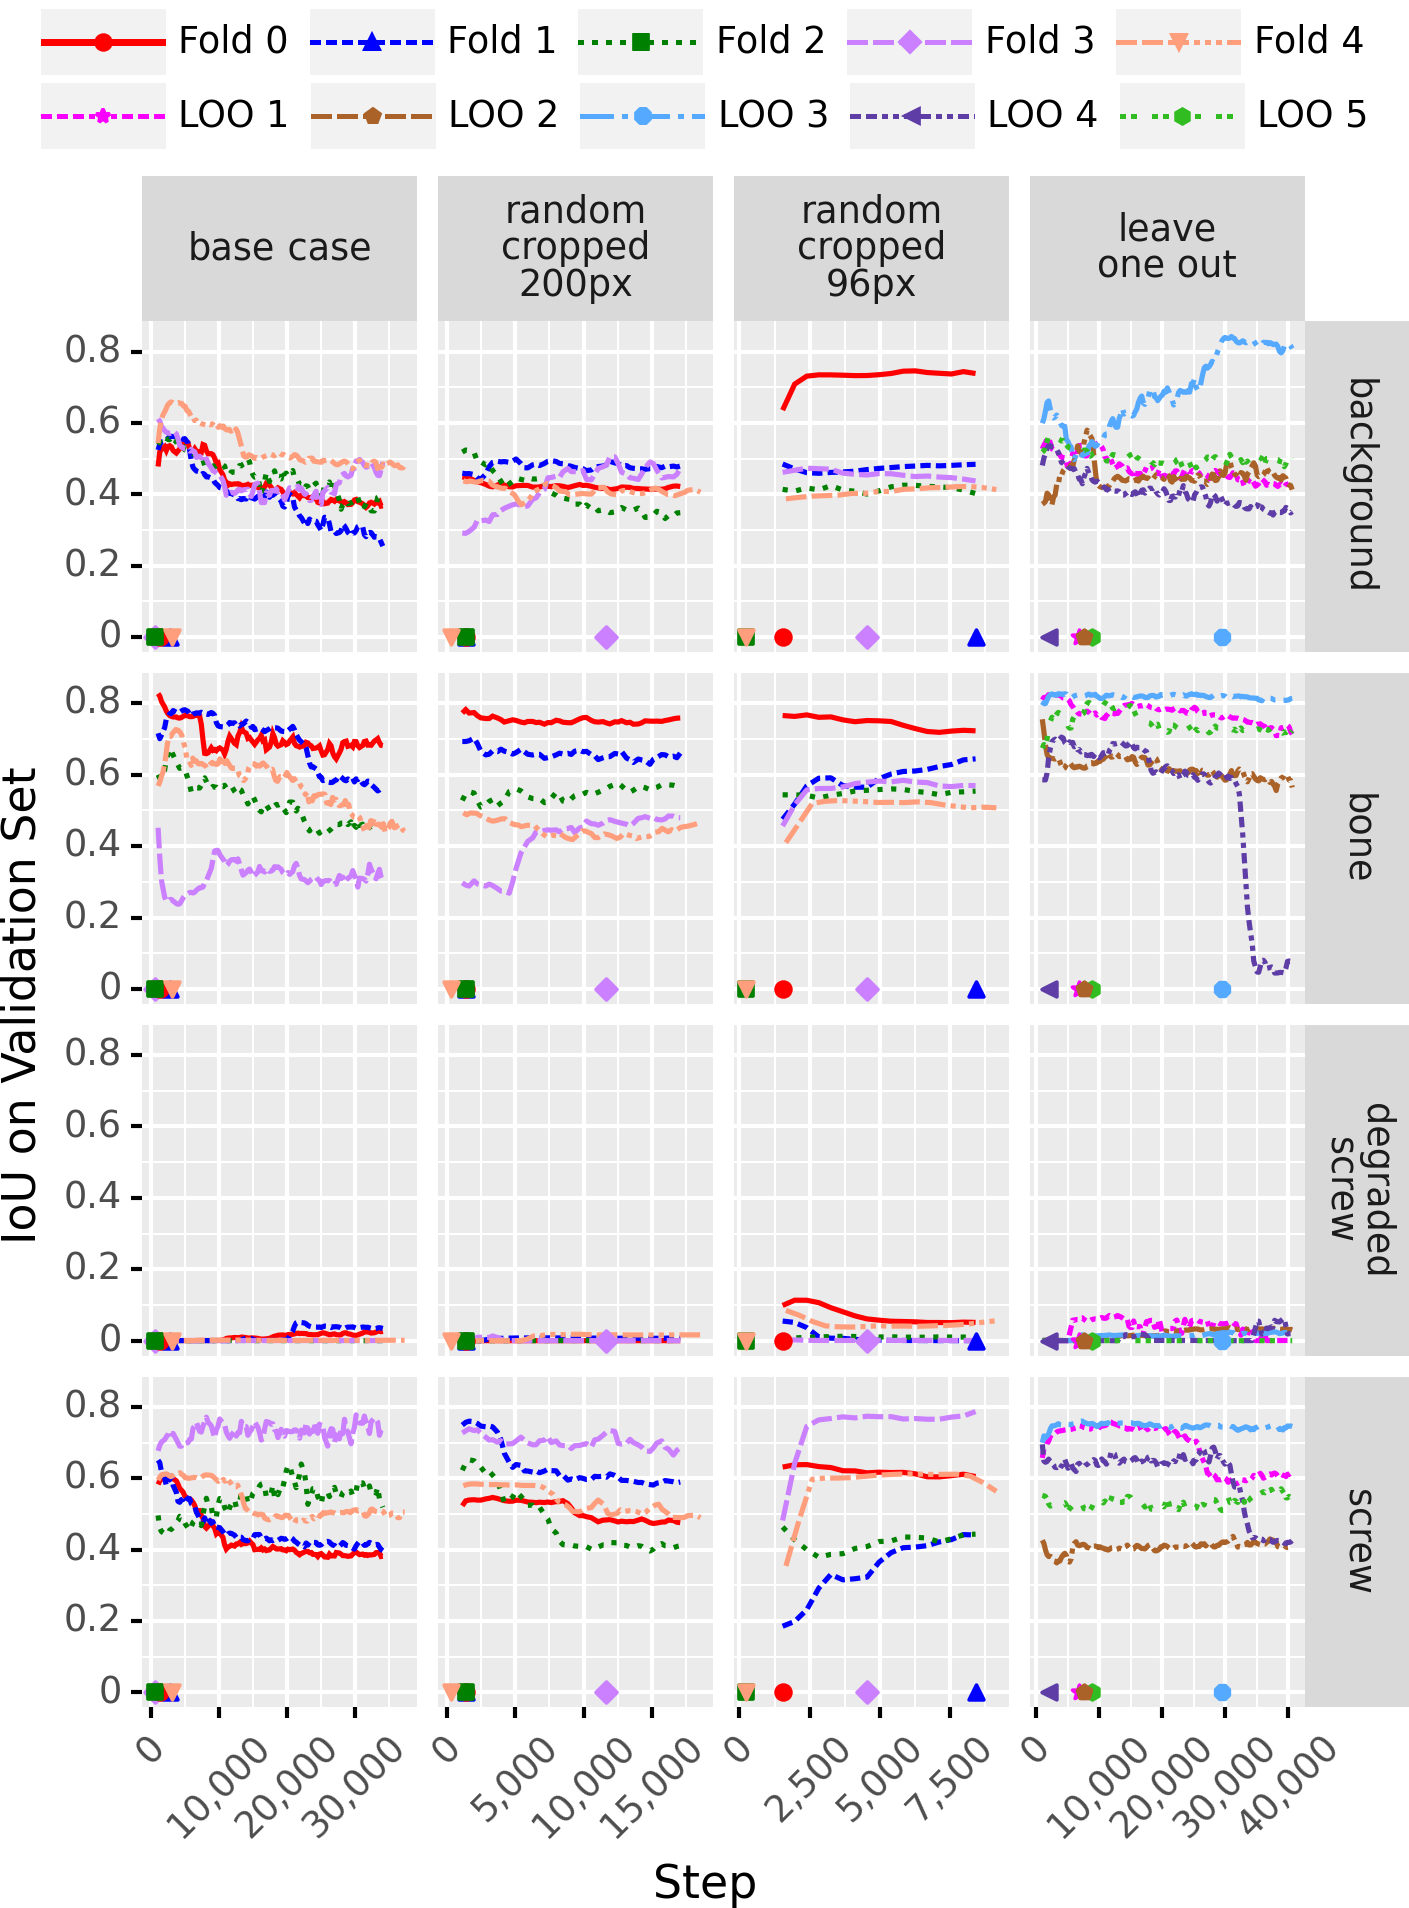
\includegraphics[width=\textwidth]{pictures/experiment_2/mIoU_labels_folds_separate_base-case_final_base-case_loo_random_cropped_final_random_cropped_res96_final}\\
    \caption[Fold- and Label-wise Development of IoU]{Fold- and label-wise development of IoU. For each cross-validation the moving average (over three data points) of the IoU per label and fold is displayed. So the first three data points are not depicted in the plots. Additionally, on the x-axis the step number of the best overall model per fold (in terms of mIoU) is marked.}
    \label{fig:miou-per-fold-label}
\end{figure}

\clearpage
\subsection{Fold-wise Development of Accuracy}
\begin{figure}[!hb]
    \centering  %trim={<left> <lower> <right> <upper>}
    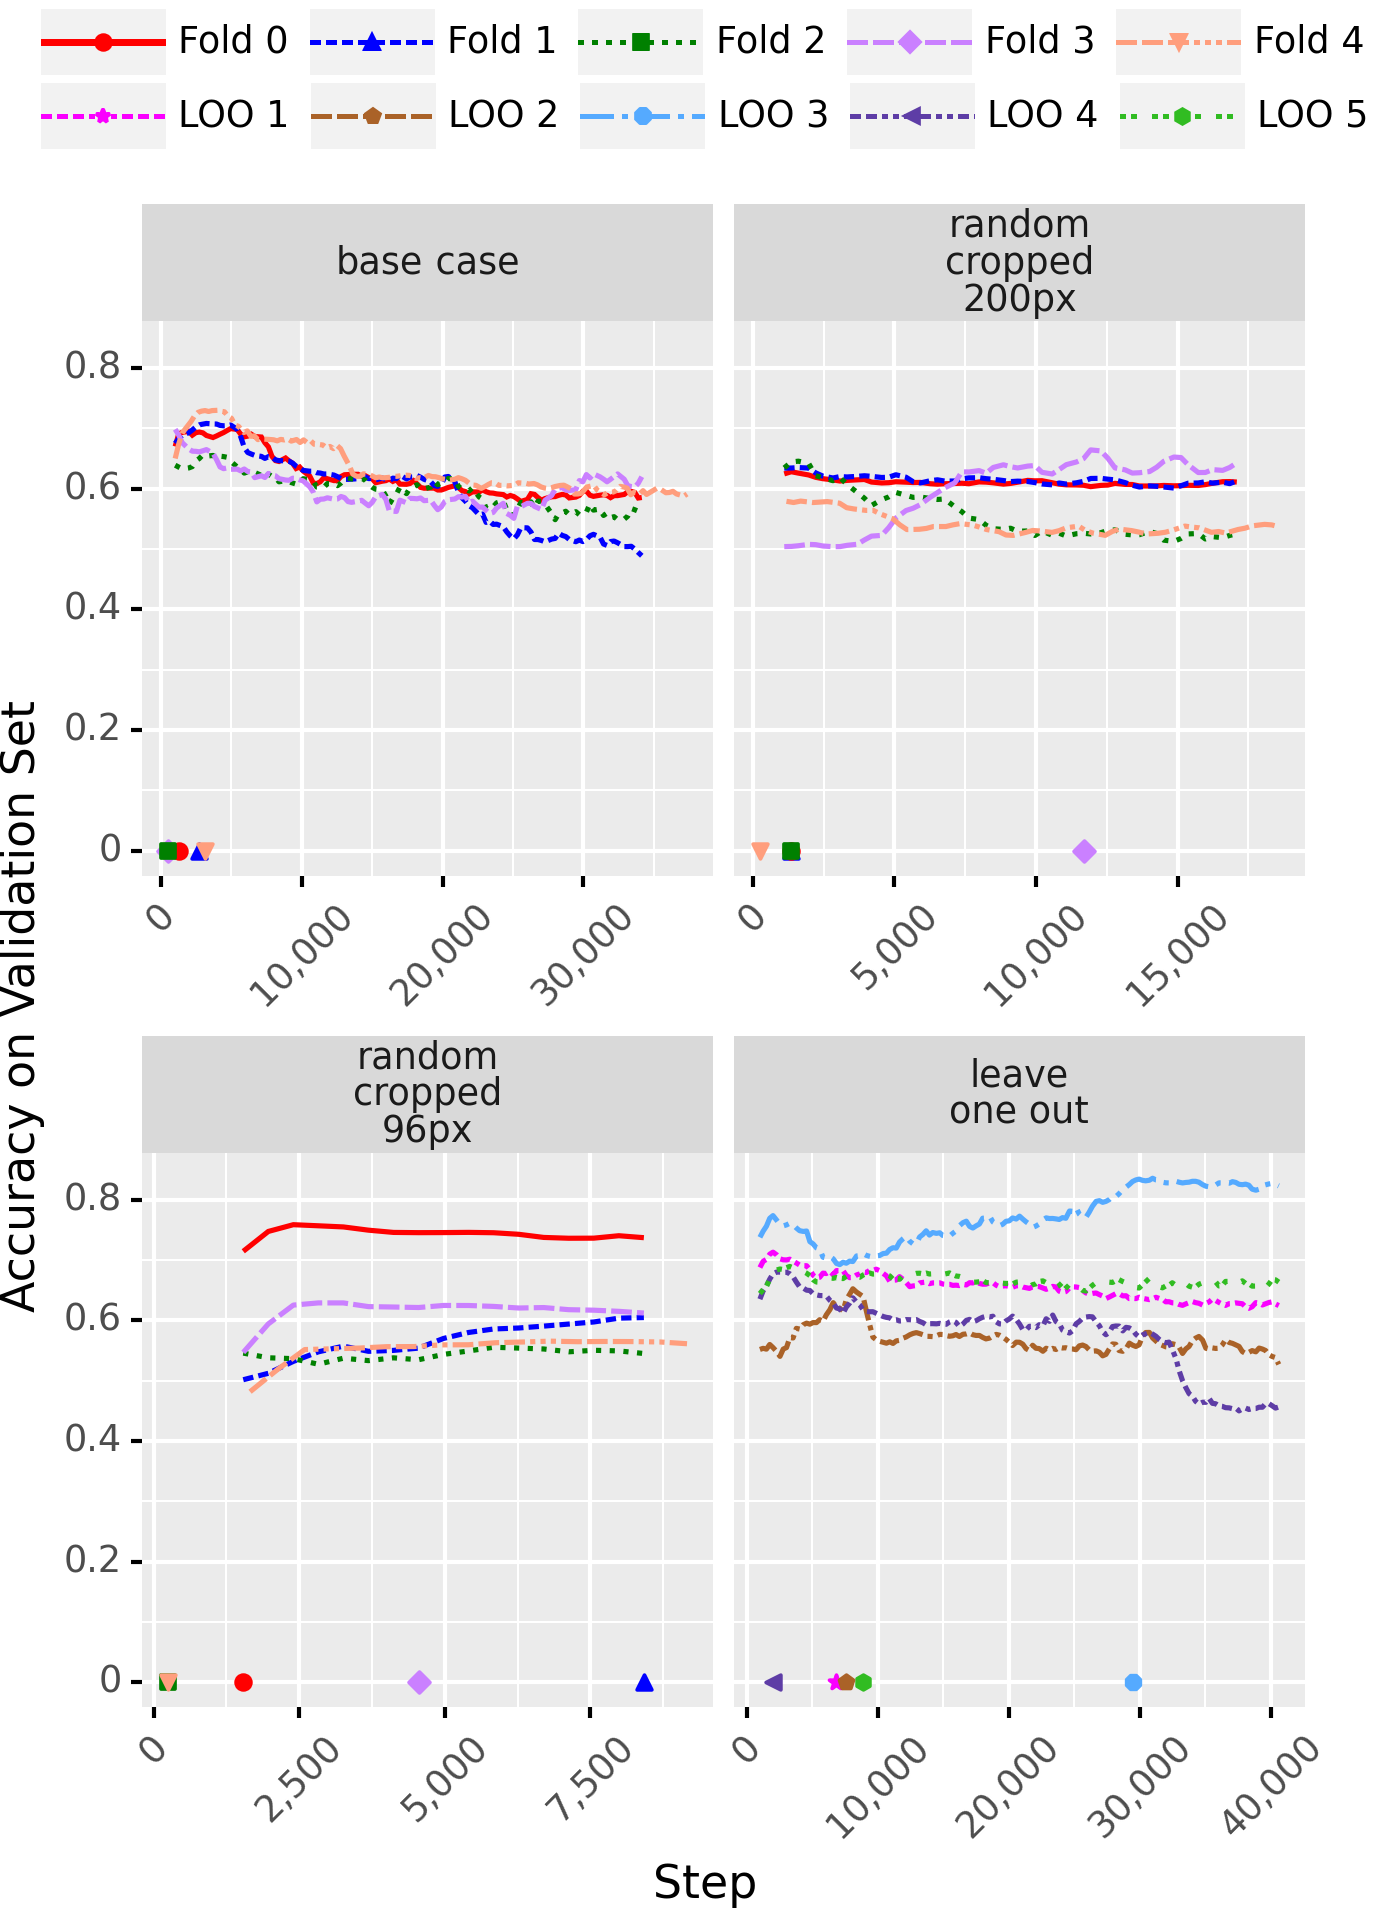
\includegraphics[width=0.95\textwidth]{pictures/experiment_2/accuracy_base-case_final_base-case_loo_random_cropped_final_random_cropped_res96_final}\\
    \caption[Fold-wise Development of Accuracy]{Fold-wise development of Accuracy. For each cross-validation the moving average (over three data points) of the Accuracy per fold is displayed. So the first three data points are not depicted in the plots. Additionally, on the x-axis the step number of the best overall model per fold (in terms of mIoU) is marked. Note, that Accuracy takes nearly the same course as mIoU just shifted upwards. }
    \label{fig:accuracy-per-fold}
\end{figure}

\clearpage
\subsection{Example Predictions for Trained Models}\label{subsec:example-predictions-for-cropping-regimes}
\begin{figure}[!htb]
    \centering      
                            %<left> <lower> <right> <upper>
    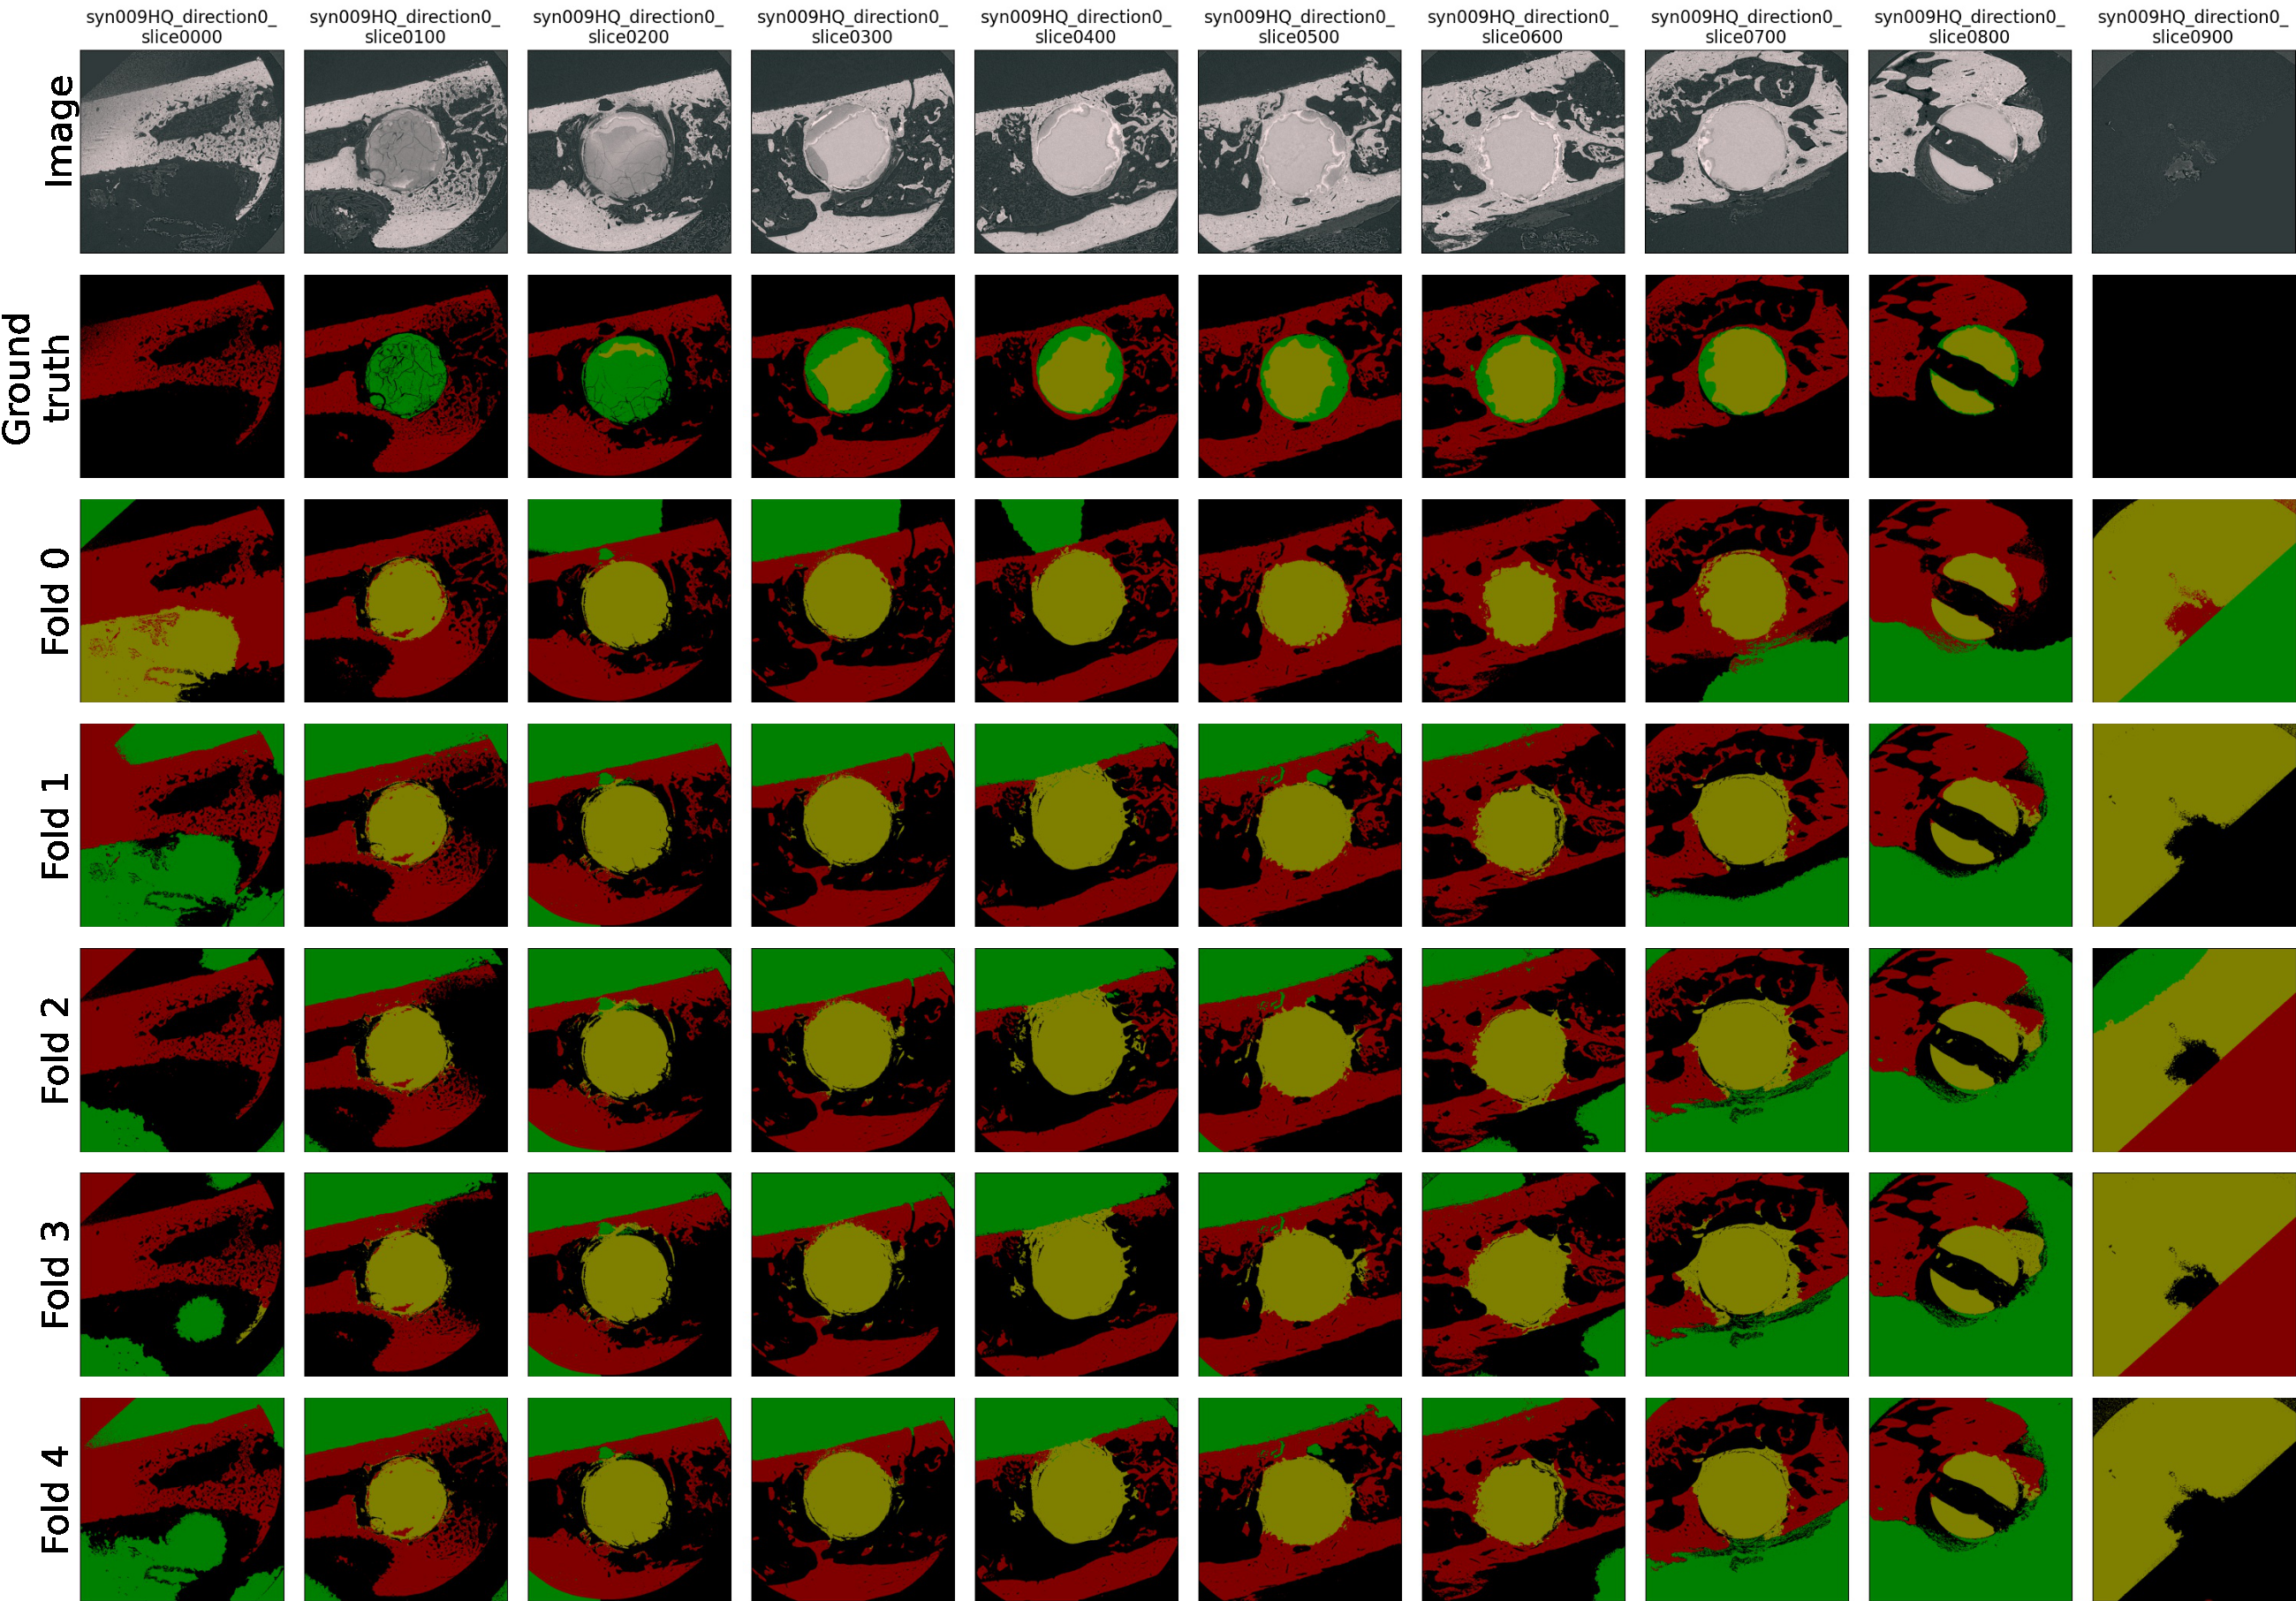
\includegraphics[clip,trim={0 0 0 7}, height=0.98\textwidth, angle=90]{pictures/experiment_2/base-case_final_example_predictions_2_all_folds}\\
    \caption[Predictions with Base Case]{Image, ground truth, and predictions of base-case (from each fold). Shown slices belong to volume syn009 (which was neither part of train nor validation set) and are ordered according to spatial location. Every 100th slice is shown. Image rotated by 90~degree.}
    \label{fig:base-case-predictions-syn009-by-fold}
\end{figure}

\clearpage
\begin{figure}[!htb]
    \centering
    %<left> <lower> <right> <upper>
    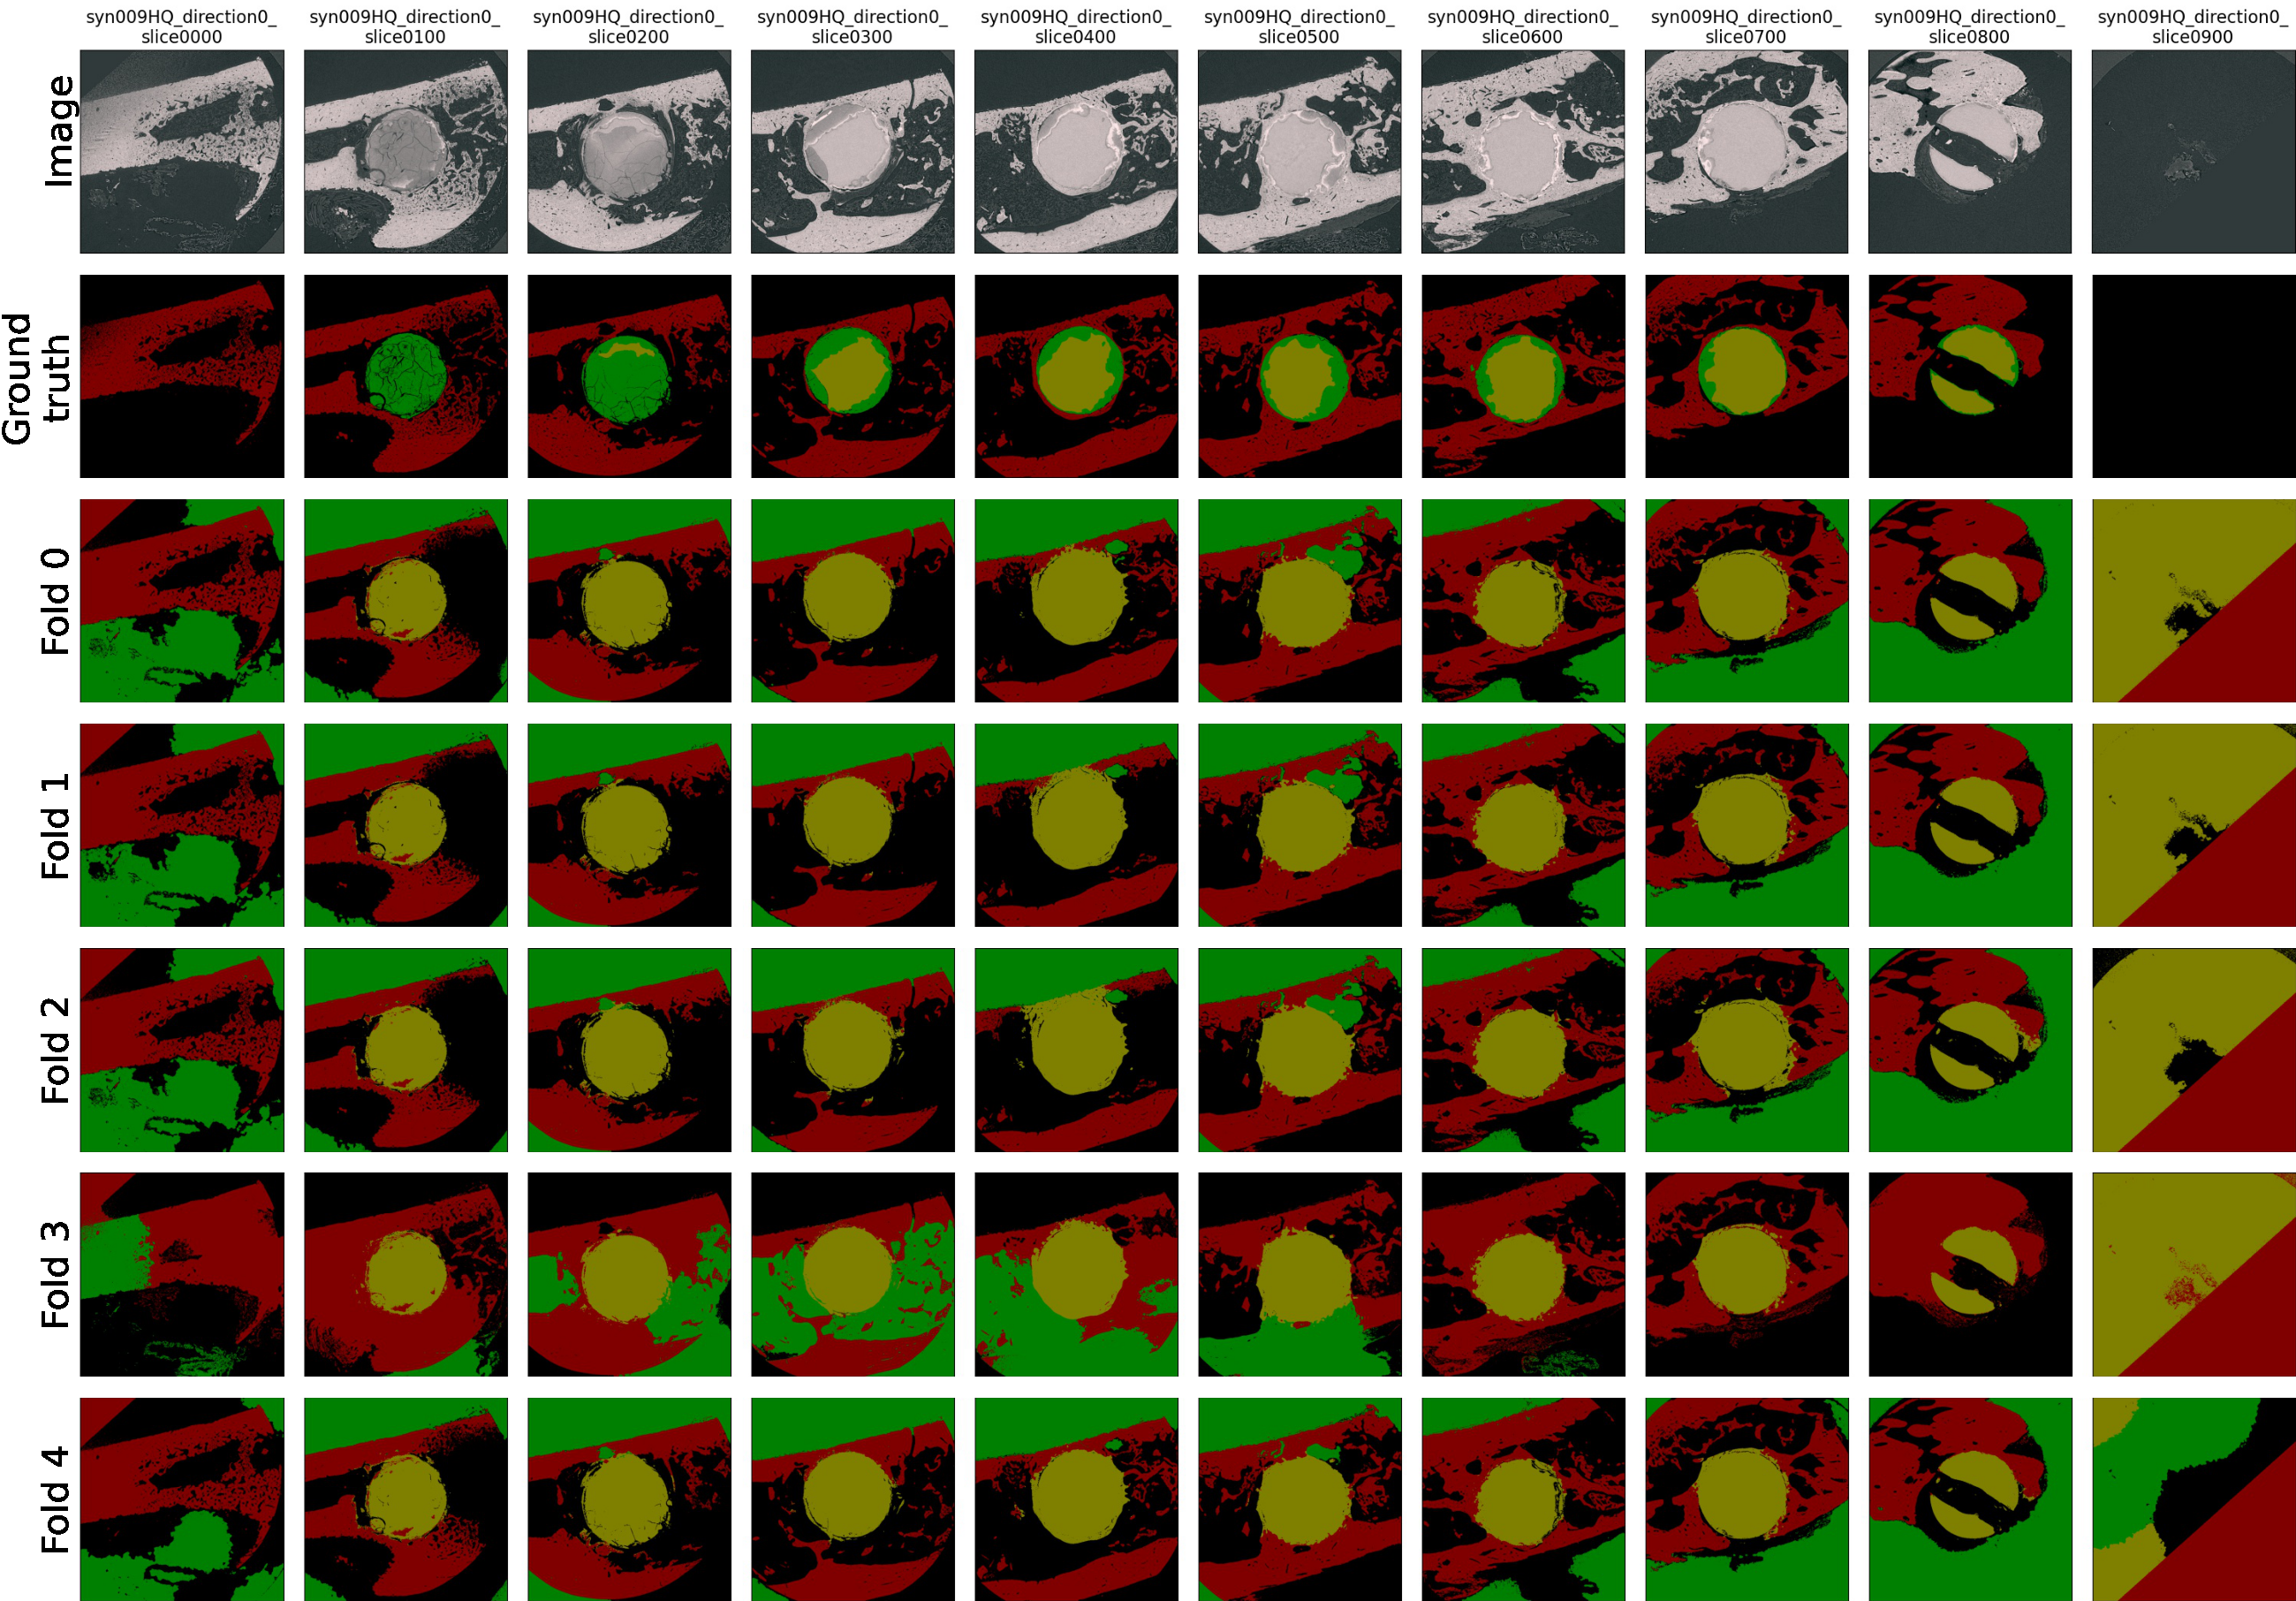
\includegraphics[clip,trim={0 0 0 7}, height=\textwidth, angle=90]{pictures/experiment_2/random_cropped_final_example_predictions_2_all_folds}\\
    \caption[Predictions with Random Cropped 200~px Regime]{Image, ground truth, and predictions of the random cropped 200~px model (from each fold).  Shown slices belong to volume syn009 (which was neither part of train nor validation set) and are ordered according to spatial location. Every 100th slice is shown. Image rotated by 90~degree.}
    \label{fig:random_cropped-predictions-syn009-by-fold}
\end{figure}

\clearpage
\begin{figure}[!htb]
    \centering
    %<left> <lower> <right> <upper>
    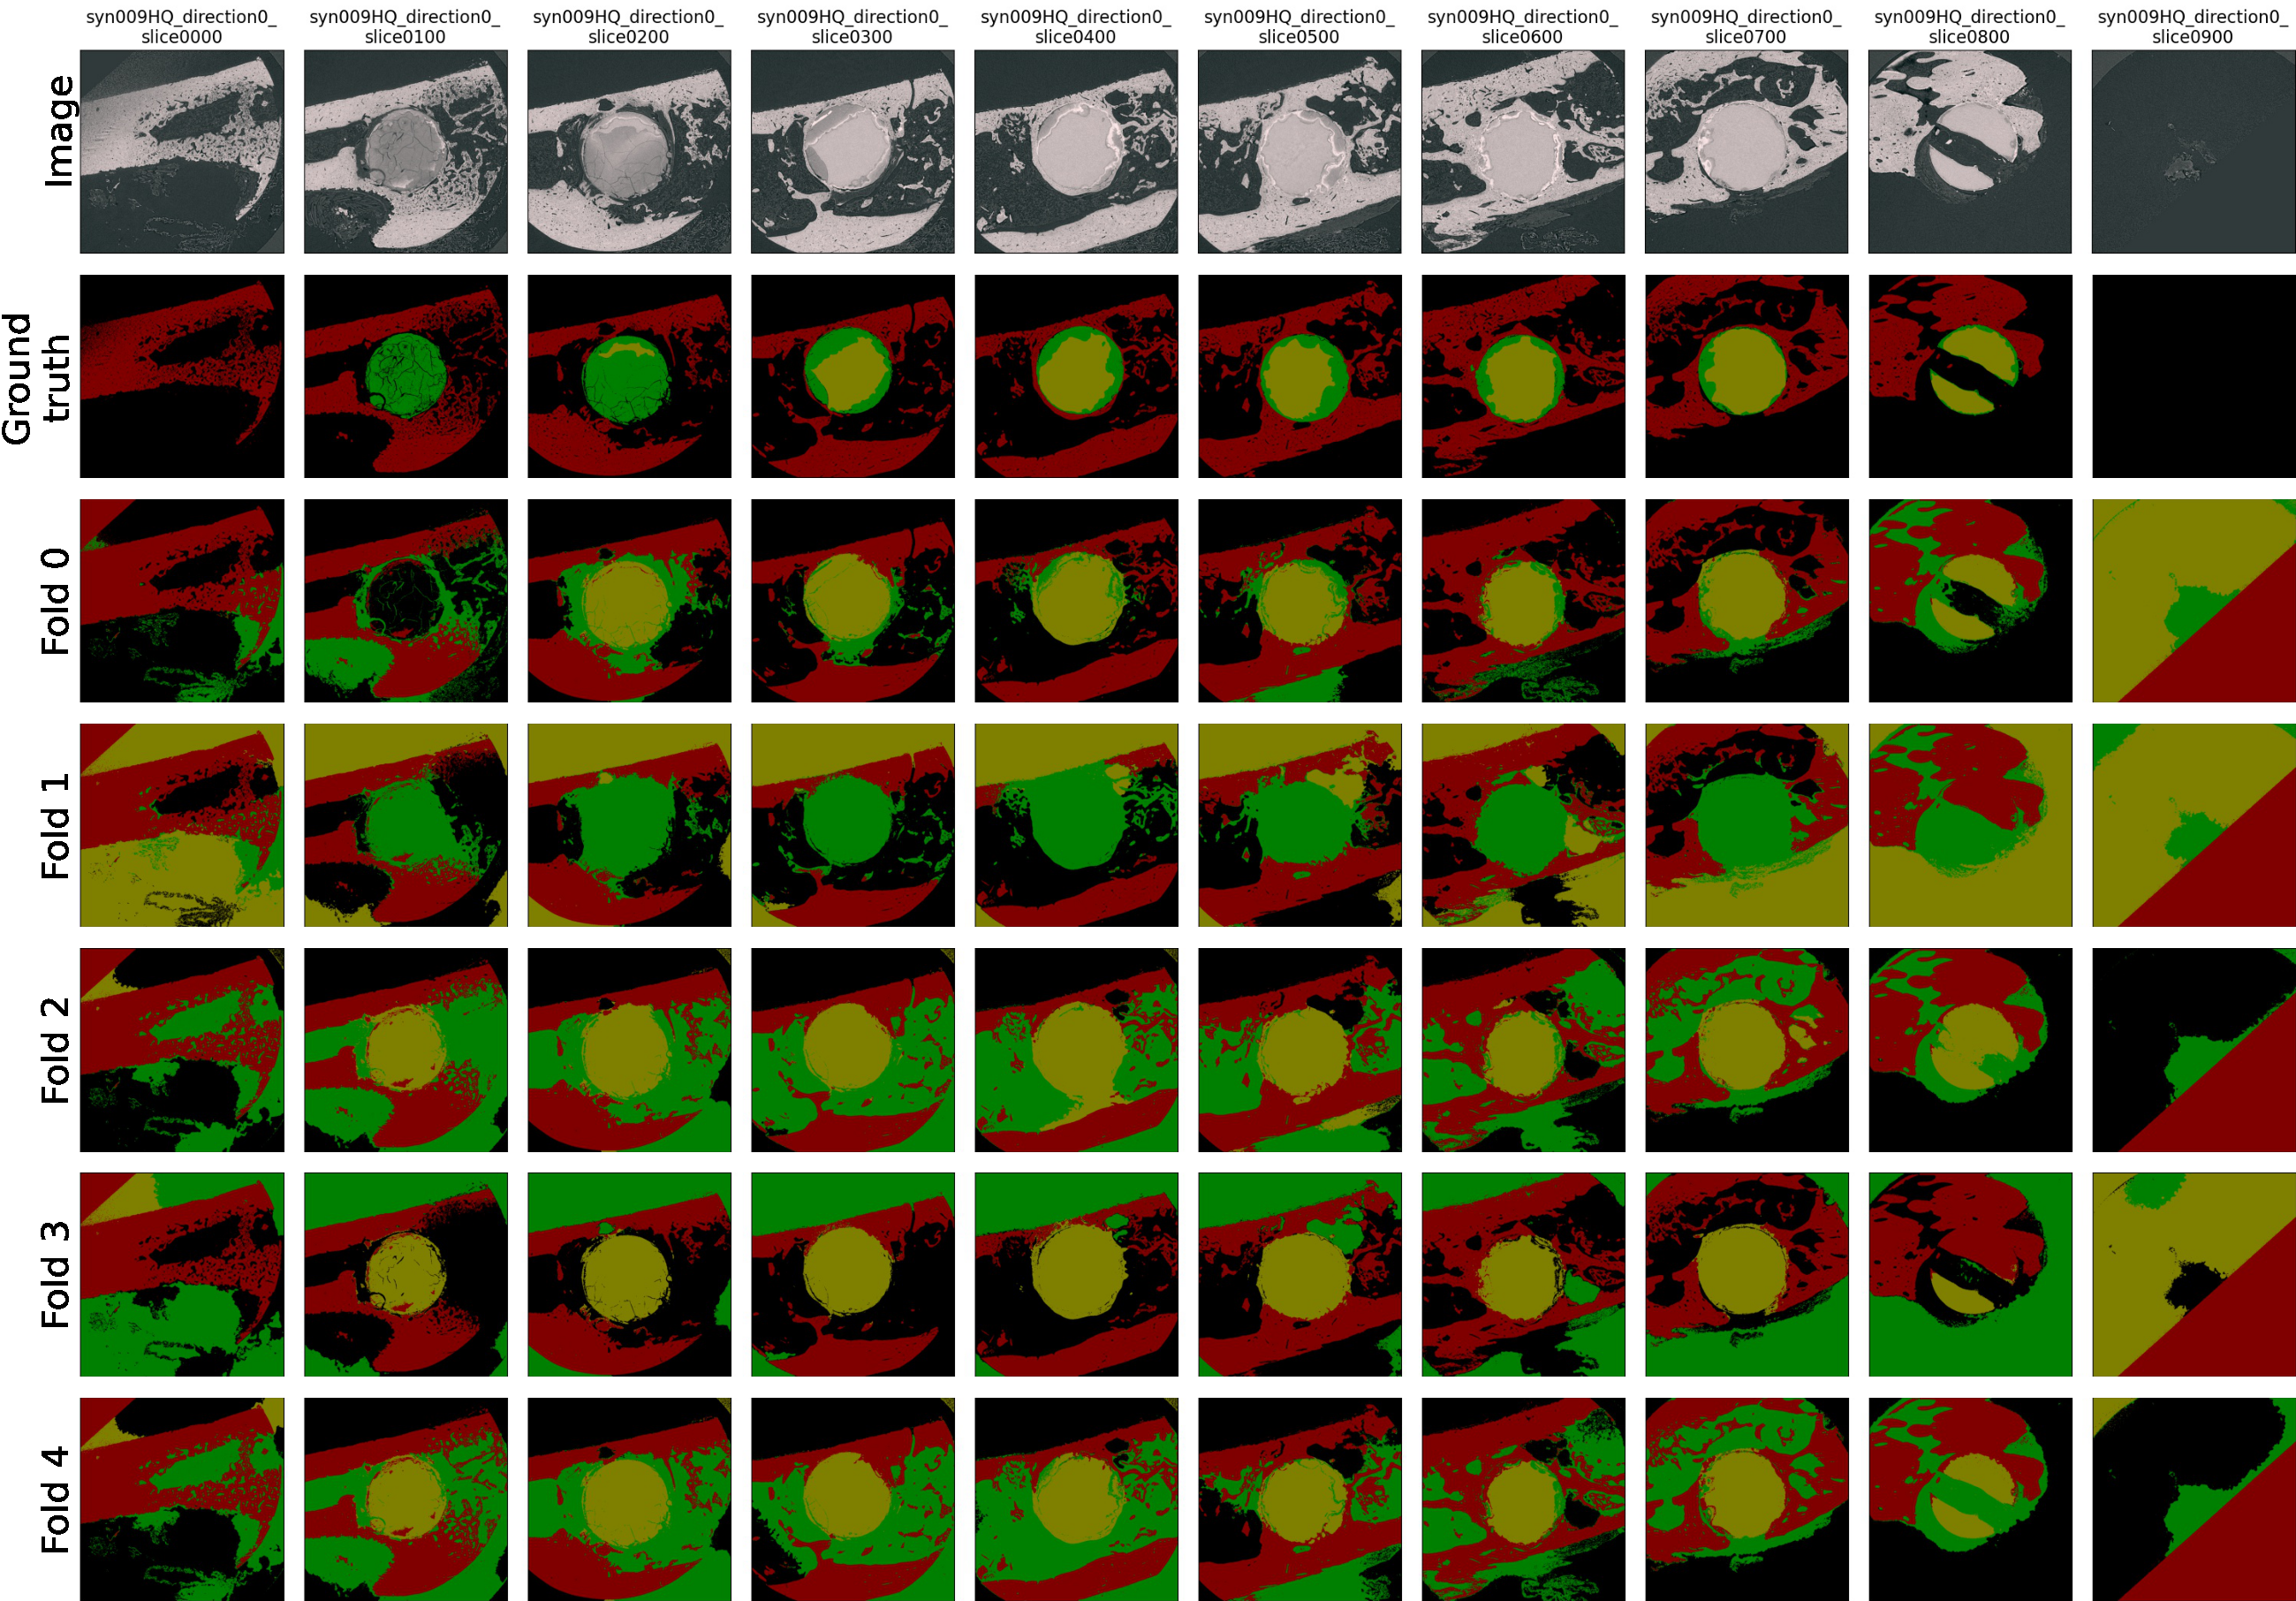
\includegraphics[clip,trim={0 0 0 7}, height=\textwidth, angle=90]{pictures/experiment_2/random_cropped_res96_final_example_predictions_2_all_folds}\\
    \caption[Predictions with Random Cropped 96~px Regime]{Image, ground truth, and predictions of the random cropped 96~px model (from each fold). Shown slices belong to volume syn009 (which was neither part of train nor validation set) and are ordered according to spatial location. Every 100th slice is shown. Image rotated by 90~degree.}
    \label{fig:random_cropped_96-predictions-syn009-by-fold}
\end{figure}

\clearpage
\begin{figure}[!htb]
    \centering
    %<left> <lower> <right> <upper>
    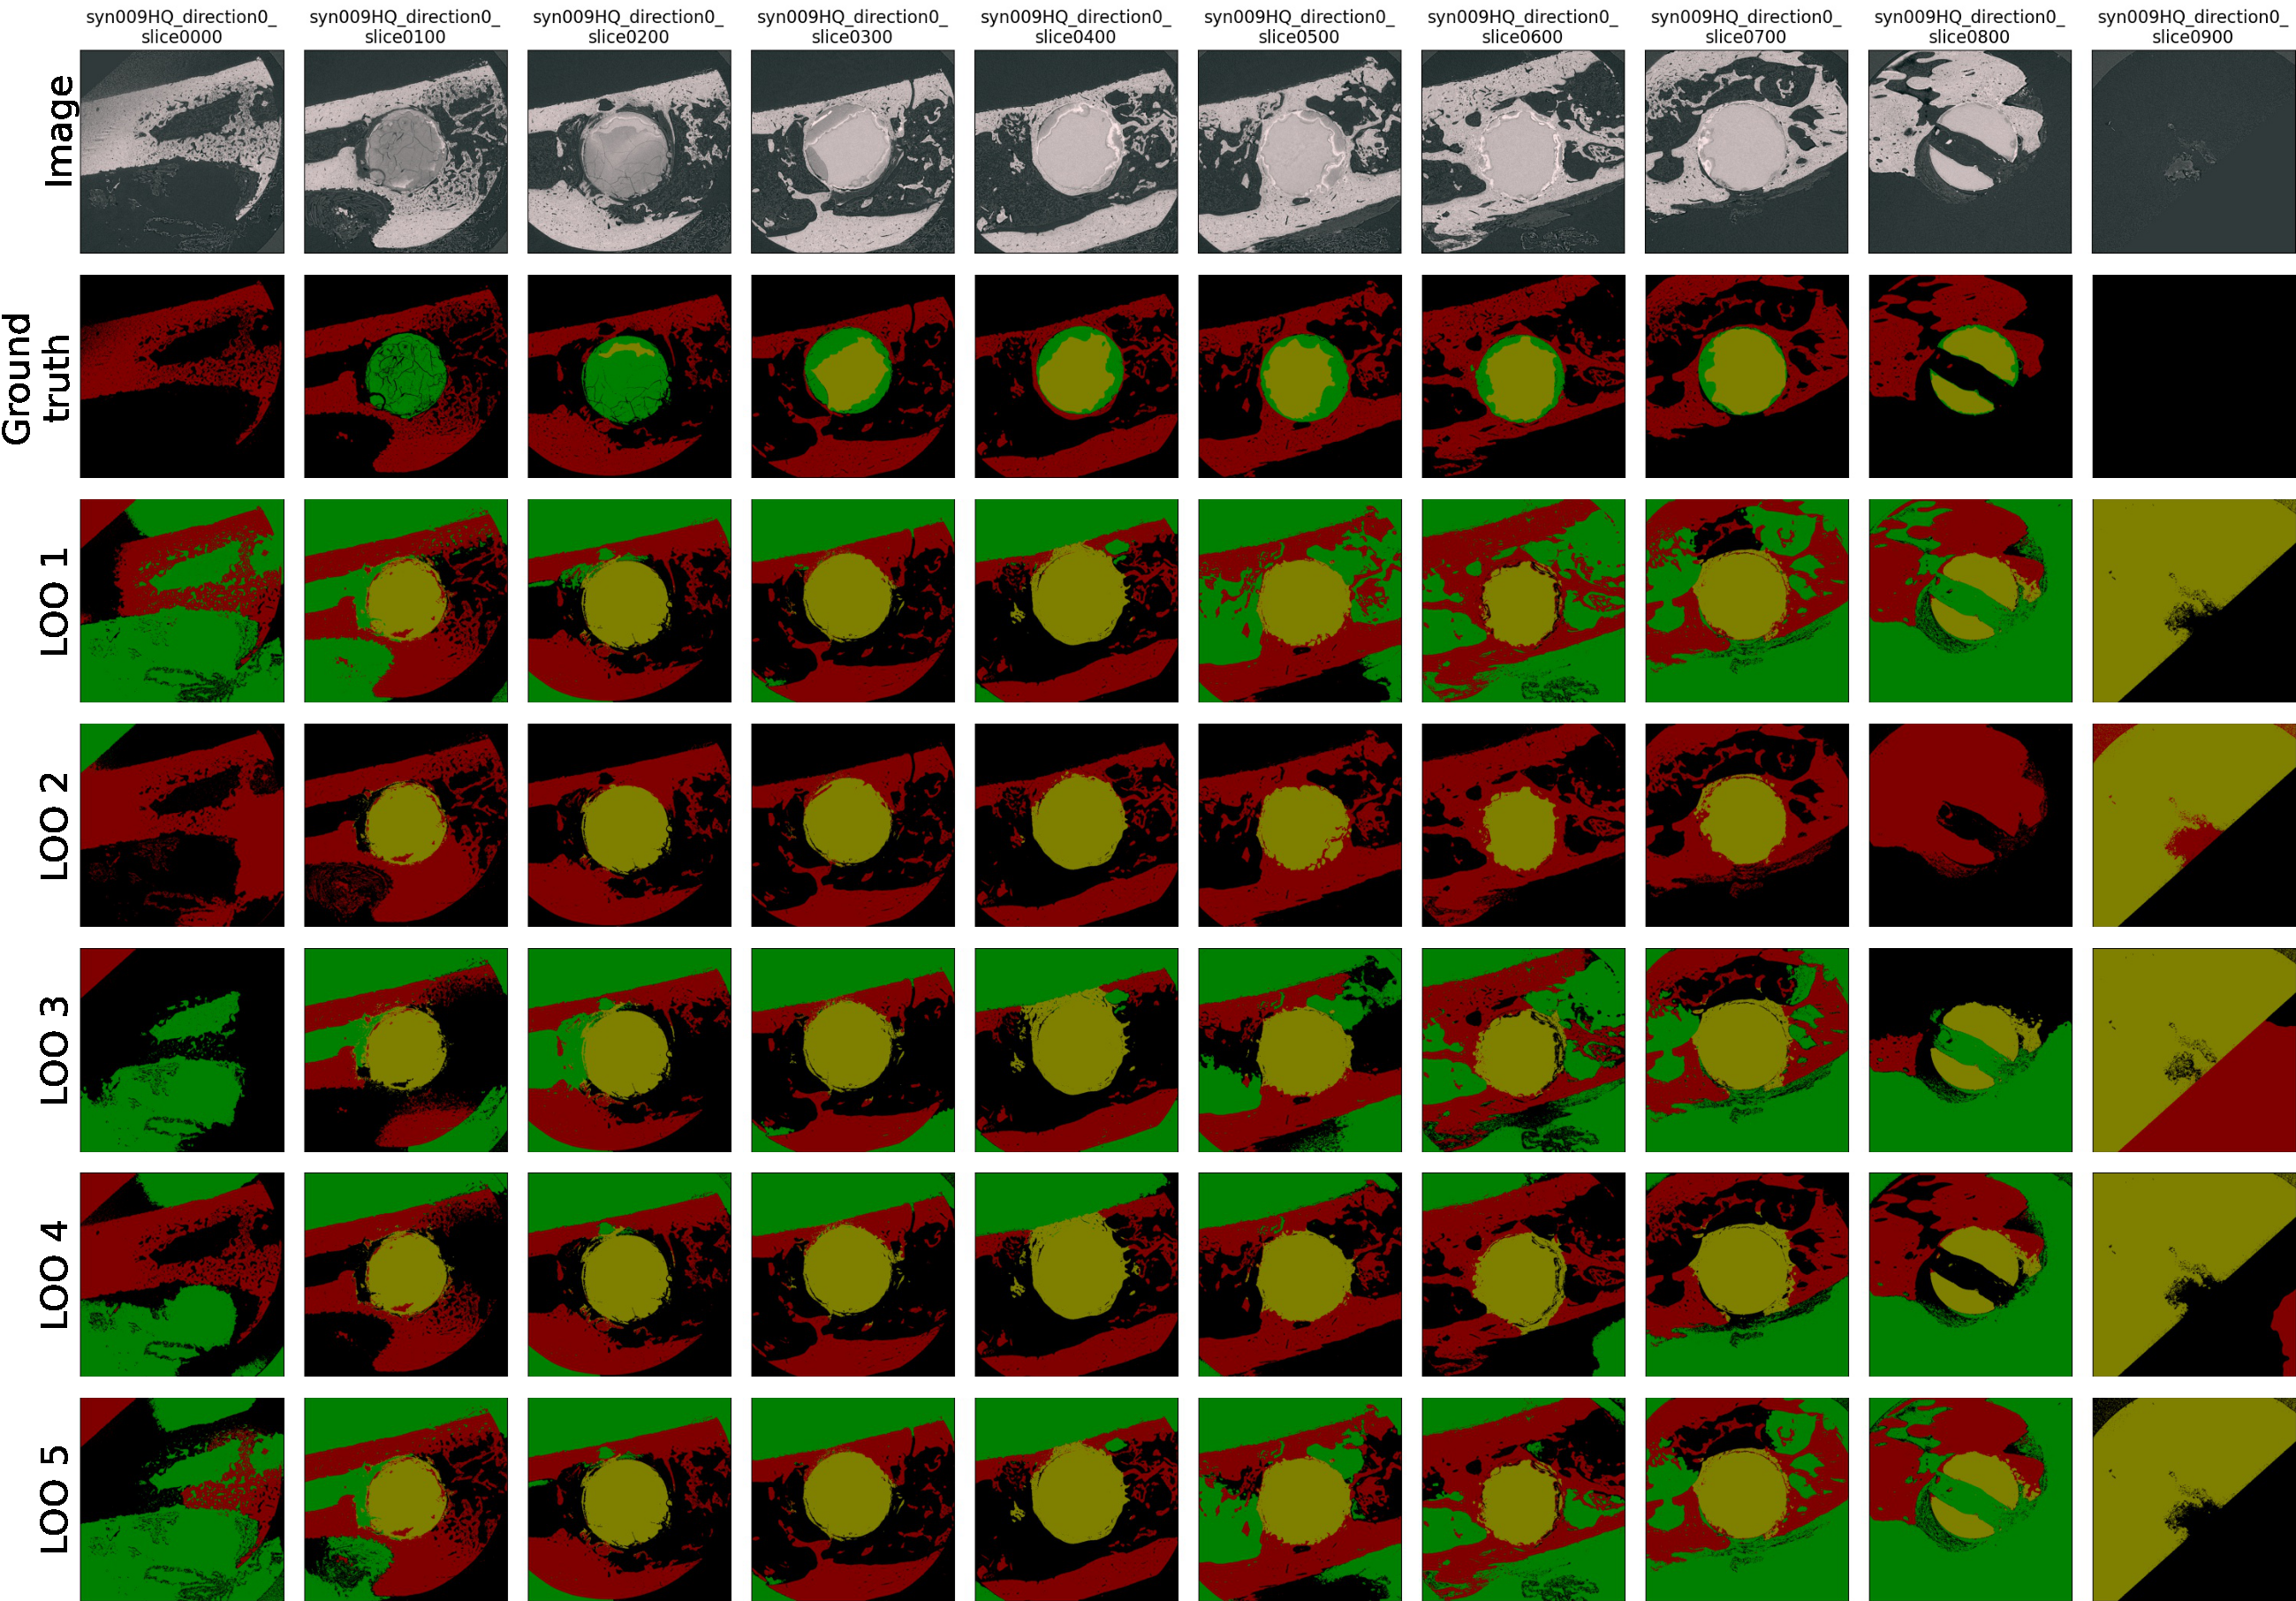
\includegraphics[clip,trim={0 0 0 7}, height=\textwidth, angle=90]{pictures/experiment_2/base-case_LOO_example_predictions_2_all_folds}\\
    \caption[Predictions with Leave-one-out Cross-validation]{Image, ground truth, and predictions of the leave-one-out cross-validation model (from each fold). Shown slices belong to volume syn009 (which was neither part of train nor validation set) and are ordered according to spatial location. Every 100th slice is shown. Image rotated by 90~degree.}
    \label{fig:loo-predictions-syn009-by-fold}
\end{figure}

\clearpage
\begin{figure}[!htb]
    \centering
    %<left> <lower> <right> <upper>
    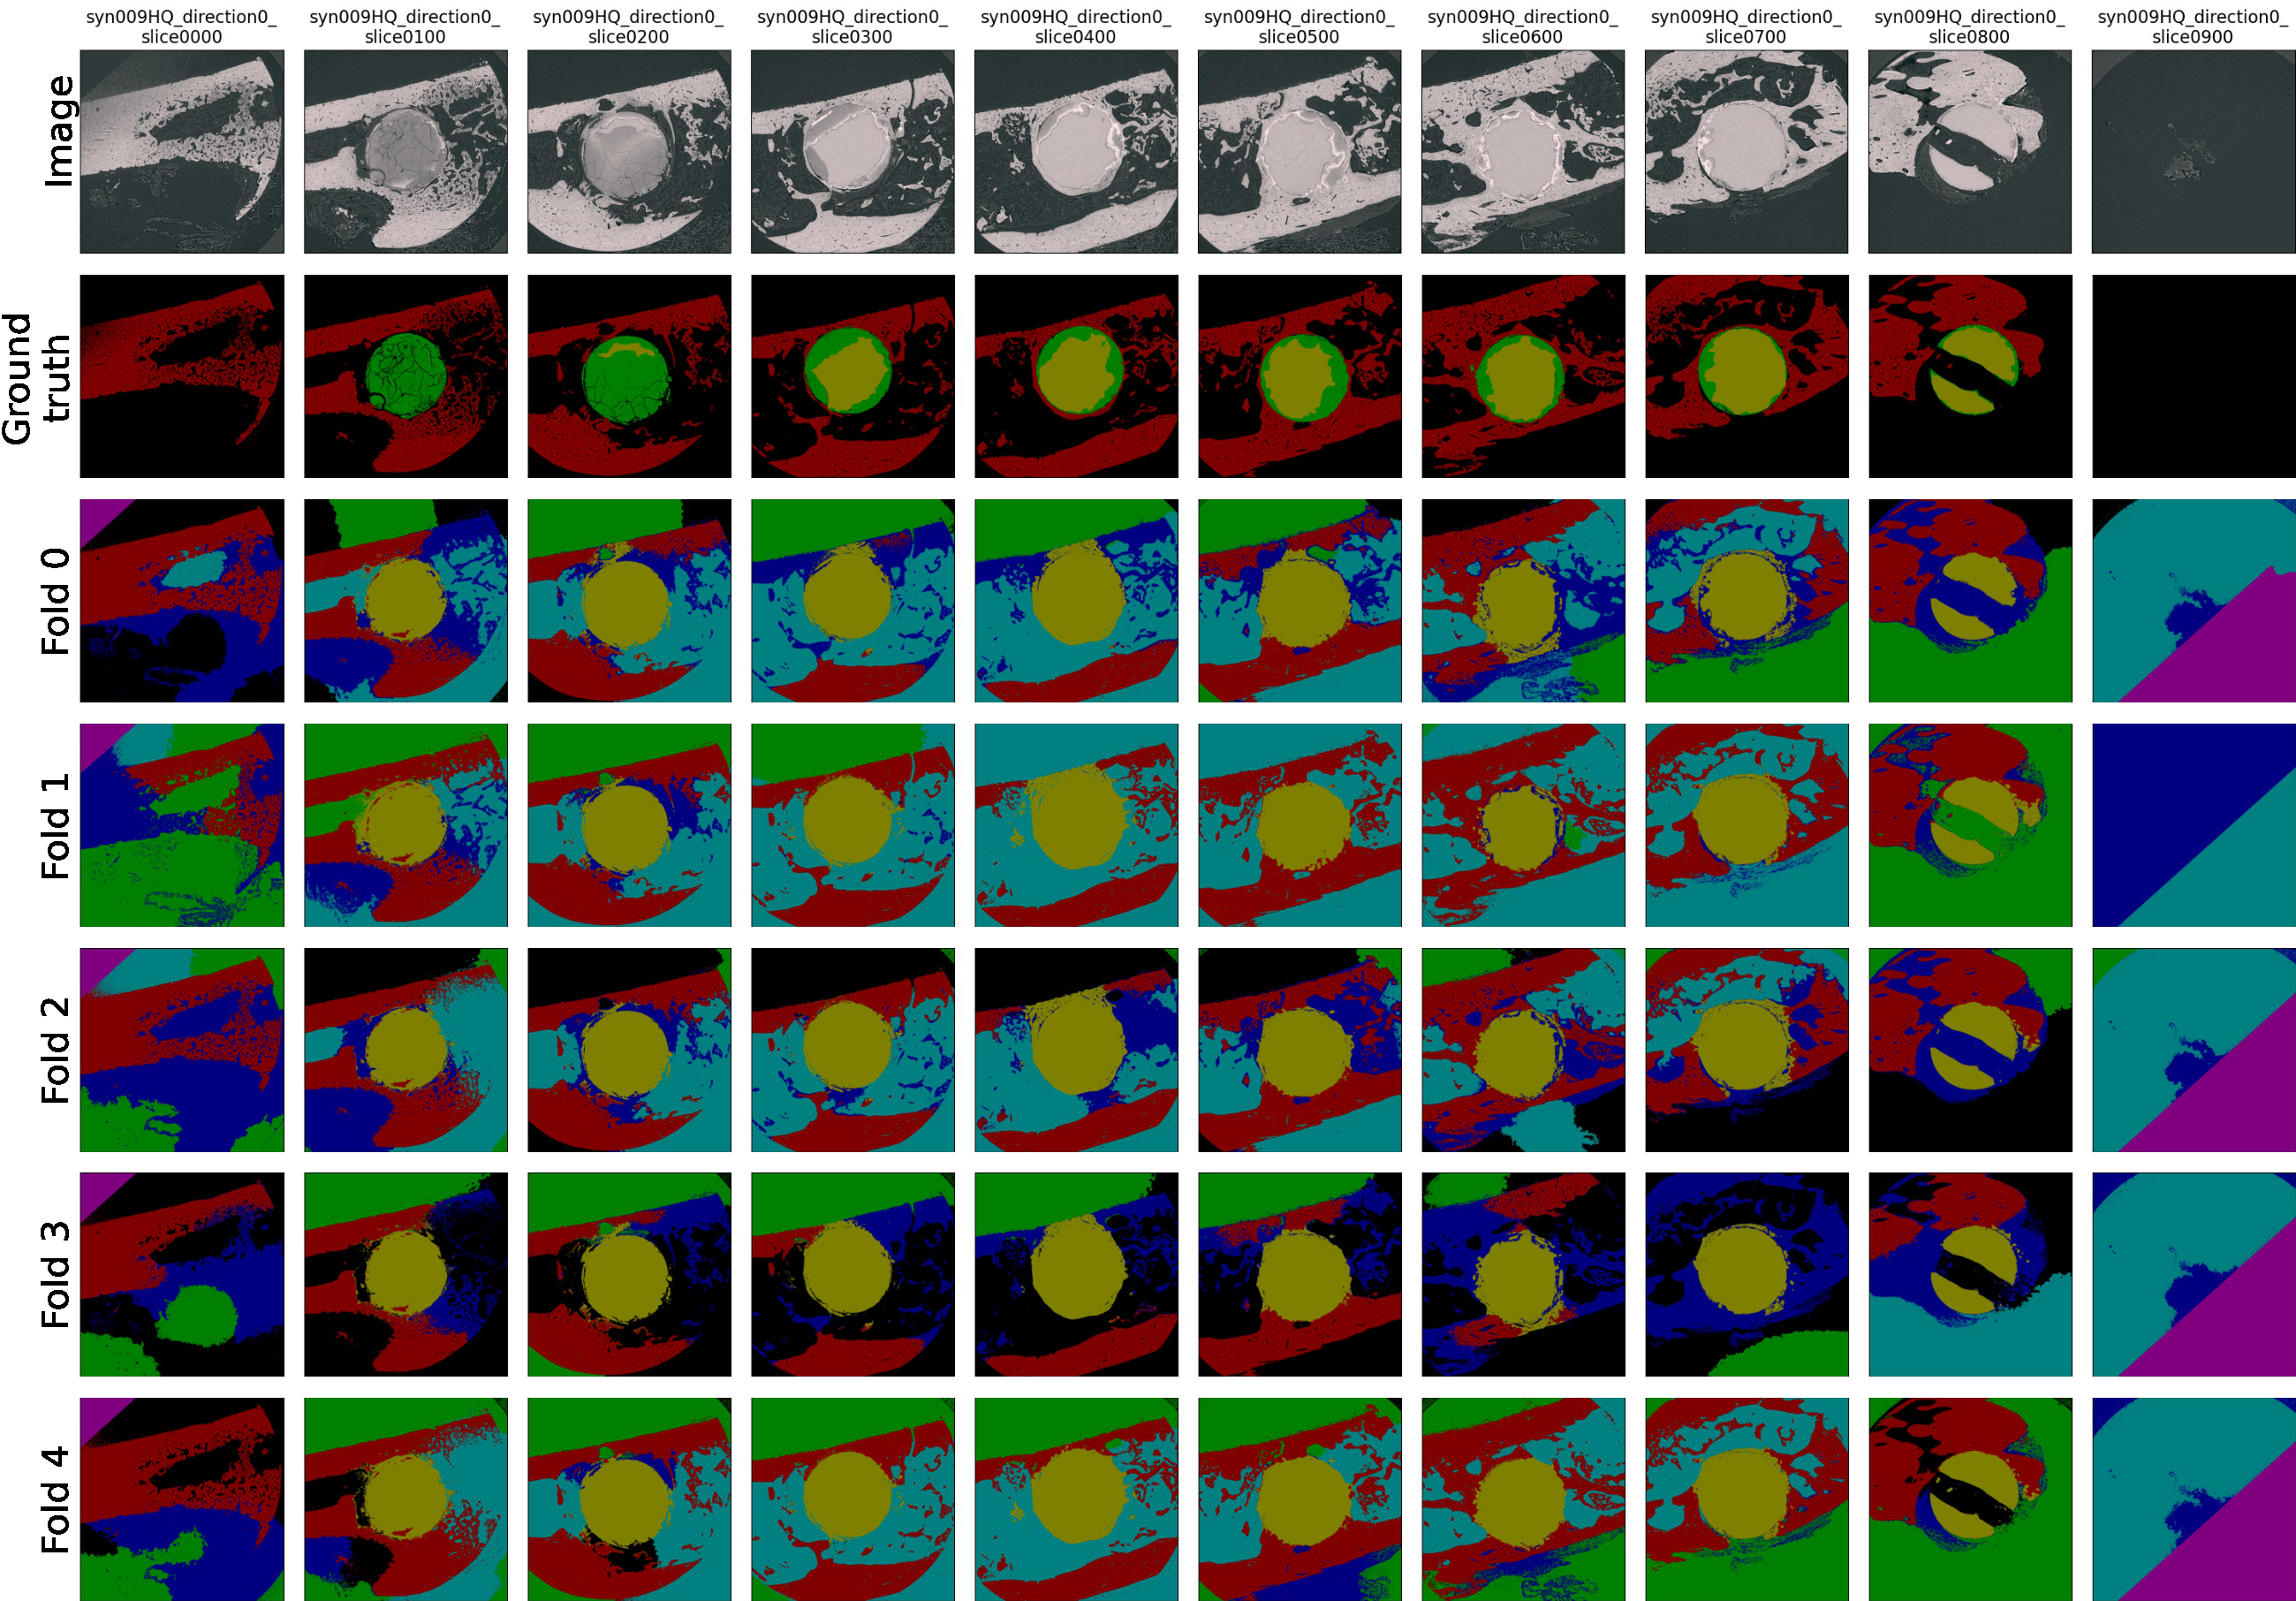
\includegraphics[clip,trim={0 0 0 7}, height=\textwidth, angle=90]{pictures/experiment_2/extra_clusters3_example_predictions_2_all_folds}\\
    \caption[Predictions with Three Extra Clusters]{Image, ground truth, and predictions of the model trained with 3 extra clusters (predictions from each fold). Shown slices belong to volume syn009 (which was neither part of train nor validation set) and are ordered according to spatial location. Every 100th slice is shown. Image rotated by 90~degree.}
    \label{fig:extra_clusters3-predictions-syn009-by-fold}
\end{figure}

\clearpage
\begin{figure}[!htb]
    \centering
    %<left> <lower> <right> <upper>
    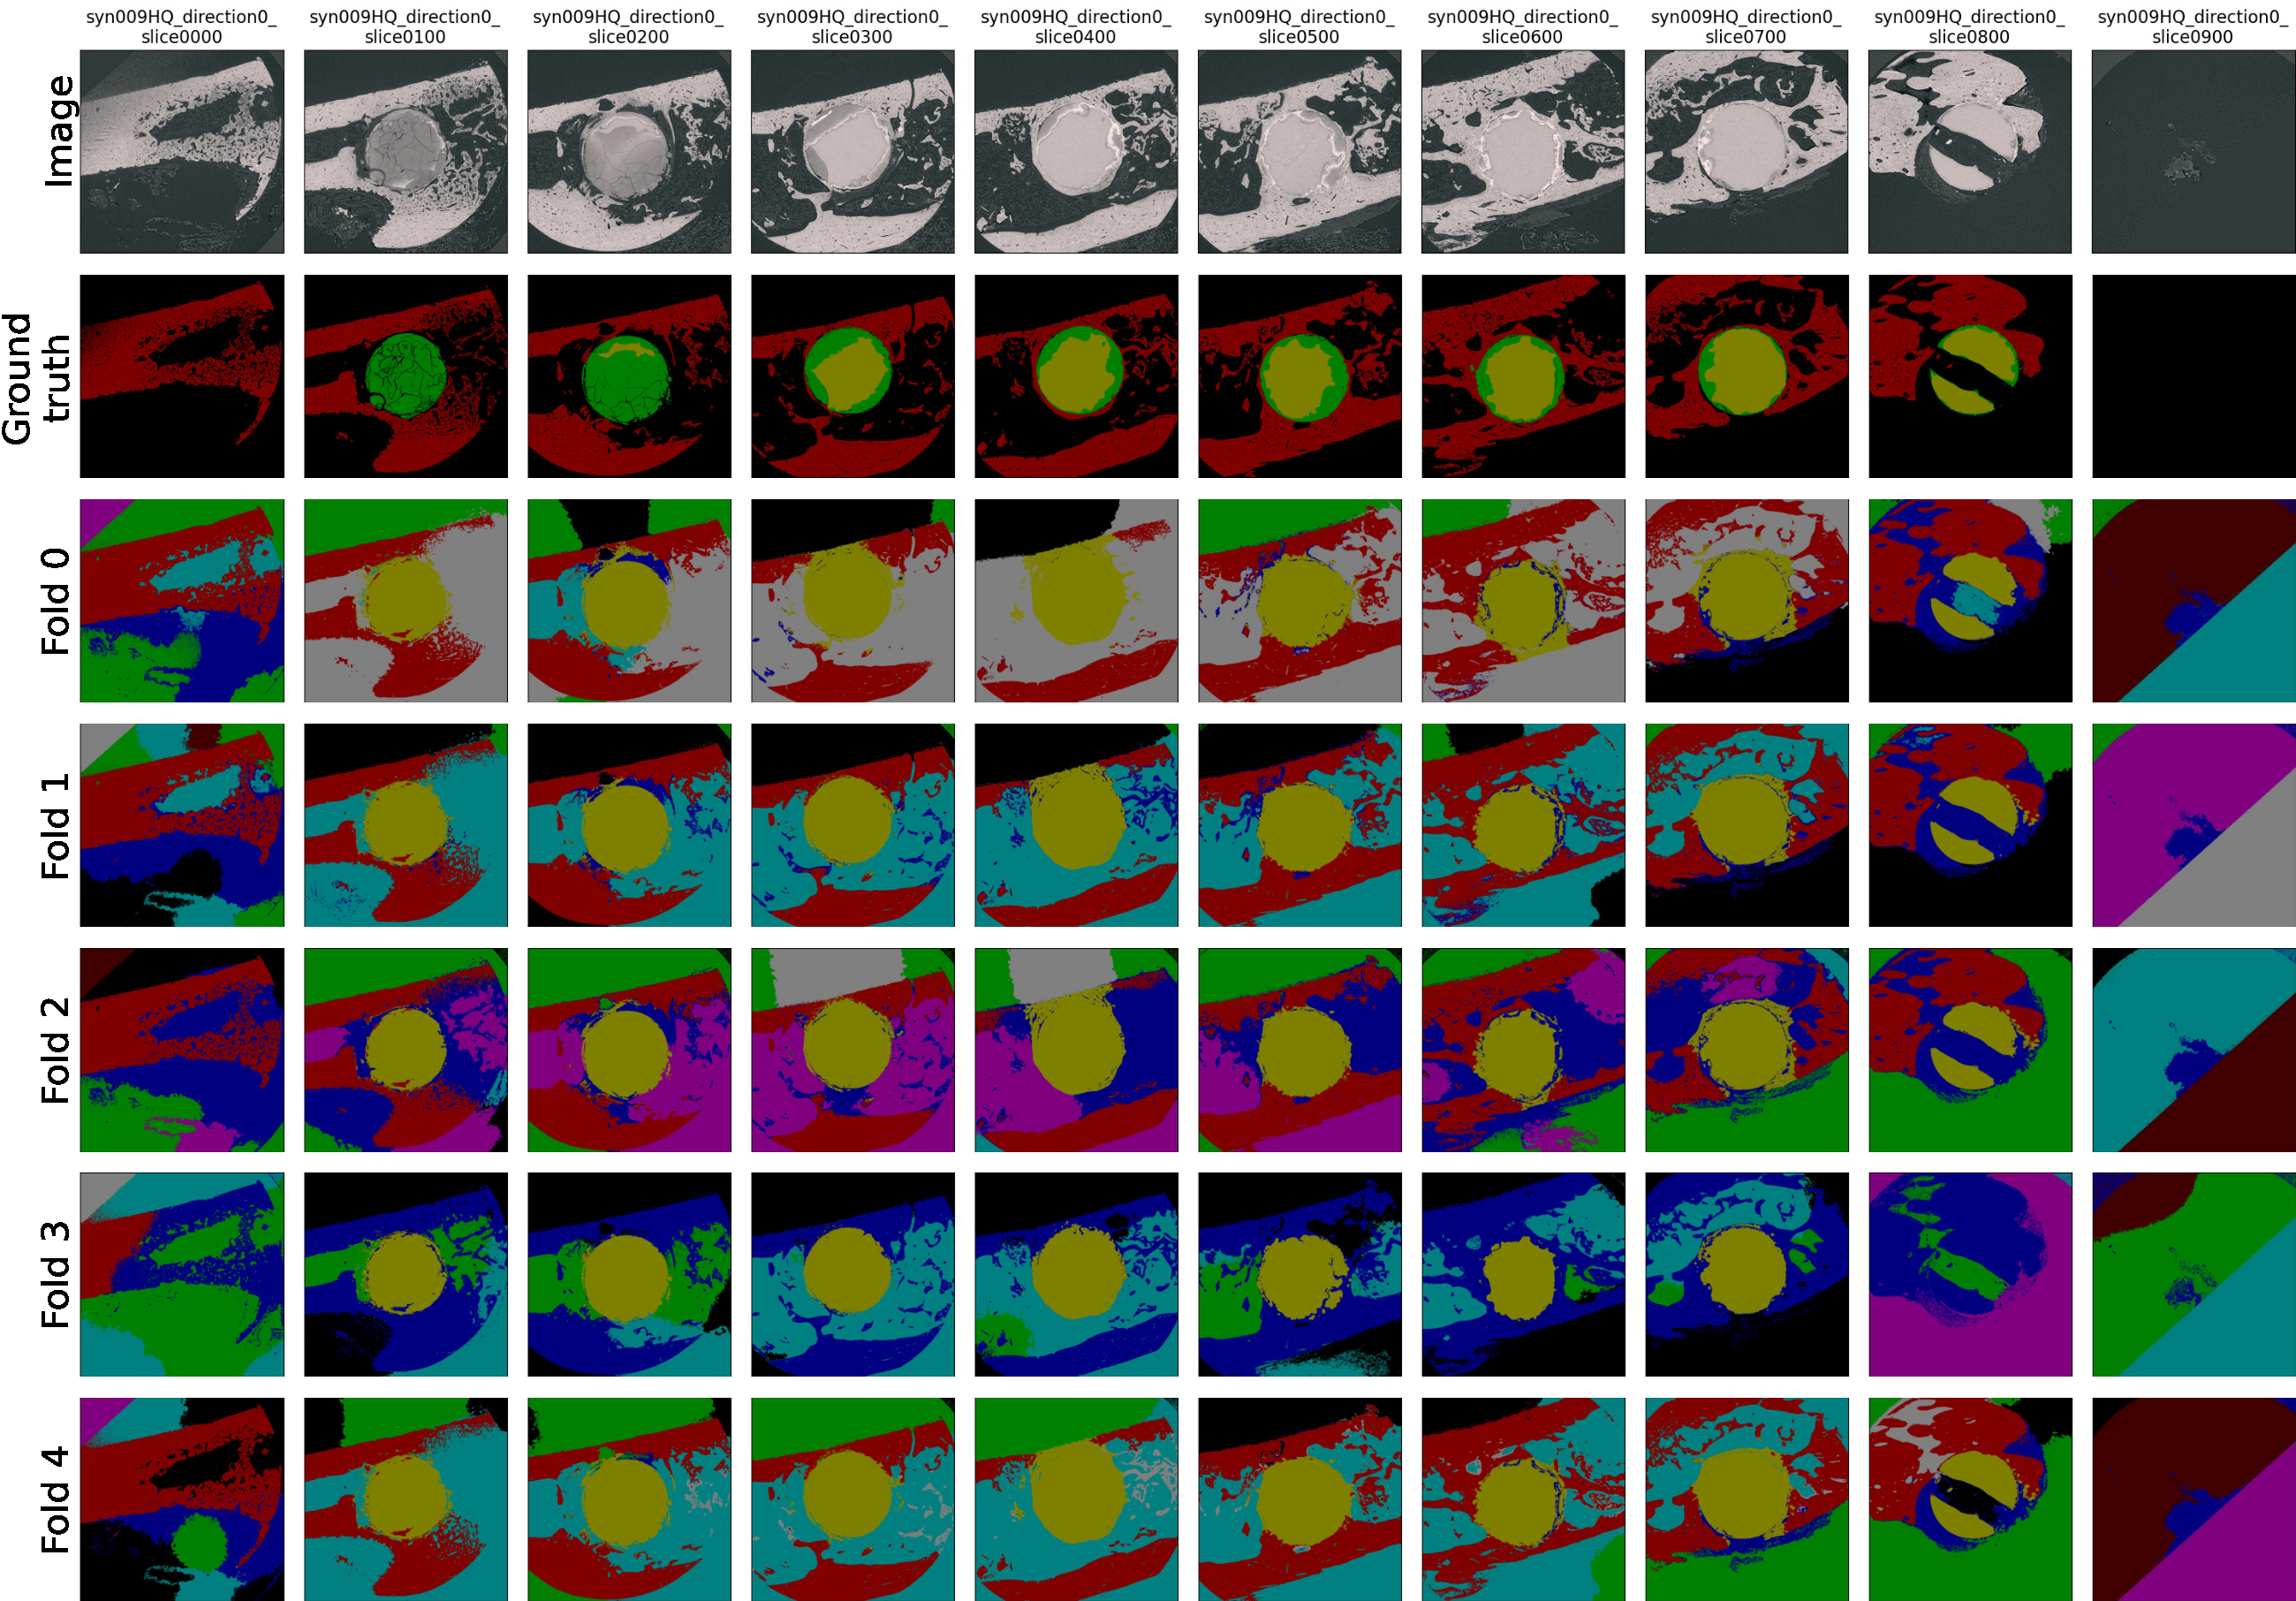
\includegraphics[clip,trim={0 0 0 7}, height=\textwidth, angle=90]{pictures/experiment_2/extra_clusters5_example_predictions_2_all_folds}\\
    \caption[Predictions with Five Extra Clusters]{Image, ground truth, and predictions of the model trained with 5 extra clusters (predictions from each fold). Shown slices belong to volume syn009 (which was neither part of train nor validation set) and are ordered according to spatial location. Every 100th slice is shown. Image rotated by 90~degree.}
    \label{fig:extra_clusters5-predictions-syn009-by-fold}
\end{figure}

\clearpage
\begin{figure}[!htb]
    \centering
    %<left> <lower> <right> <upper>
    \includegraphics[clip,trim={0 0 0 7}, height=\textwidth, angle=90]{pictures/experiment_2/extra_clusters10_example_predictions_2_all_folds}\\
    \caption[Predictions with Ten Extra Clusters]{Image, ground truth, and predictions of the model trained with 10 extra clusters (predictions from each fold). Shown slices belong to volume syn009 (which was neither part of train nor validation set) and are ordered according to spatial location. Every 100th slice is shown. Image rotated by 90~degree.}
    \label{fig:extra_clusters10-predictions-syn009-by-fold}
\end{figure}

\clearpage
\section*{Eidesstattliche Erklärung}
\addcontentsline{toc}{section}{Eidestattliche Erklärung}
\emph{Ich erkläre hiermit an Eides Statt, dass ich die vorliegende Arbeit selbstständig und ohne Benutzung anderer als der angegebenen Hilfs-mittel angefertigt habe; die aus fremden Quellen direkt oder indirekt übernommenen Gedanken sind als solche kenntlich gemacht.
Die Arbeit wurde bisher in gleicher oder ähnlicher Form keiner anderen Prüfungskommission vorgelegt und auch nicht veröffentlicht.}
\\
\\

Ort, Datum \hfill Unterschrift (Jennifer Ahrens)


\end{document}

